%\documentclass[10pt,a4paper,twocolumn,openany]{book}
\documentclass[10pt,a4paper,openany]{book}

\usepackage[bg-a4]{lib/rpg-book} % Options: bg-a4, bg-letter, bg-full, bg-print, bg-none.
\usepackage[english]{babel}
\usepackage{graphicx}
\usepackage{float}
\restylefloat{table}
% For the Gyre Chorus font - font code: qzc
%\usepackage{tgchorus}
%\usepackage[T1]{fontenc}
%https://tex.stackexchange.com/questions/25249/how-do-i-use-a-particular-font-for-a-small-section-of-text-in-my-document
%{\fontfamily{qzc}\selectfont
%This and that text new font
%}

\hyphenation{round-ed Stre-ngth Game-master Mind-link weap-ons}

% Start document
\begin{document}
\fontfamily{ppl}
\selectfont % Set text font
\frontmatter

\rpgMakeCover[
    image = img/cover,
    logo = img/empty,
    title = Fantasy Crux,
    subtitle = {\ttfamily \\An Open D100 System created by\\Konstantinos Karasavvas}
    %subtitle = {\ttfamily An Open D100 System created by\\~\\Konstantinos Karasavvas\\~\\{\Large based on OpenQuest by Newt Newport}}
    %subtitle = {\ttfamily An Open D100 System created by Konstantinos Karasavvas\\~\\Art by ncorva, SirenD, John Malis and Stable Cascade\\~\\{\Large based on OpenQuest by Newt Newport}}
]

%Maybe here the credits... for artists and playtesters ?

\setcounter{tocdepth}{1}
\tableofcontents

% Your content goes here
\mainmatter

\chapter{Introduction}
\label{ch:introduction}


\section{About Fantasy D100}

Fantasy D100 is a fantasy RPG game system. It is essentially my take of the great OpenQuest rules (based on the SRD version).

This has much more than my custom rules though. It has several additions and (what I believe are) cleaner mechanics that abstract any extraordinary or supernatural abilities (like magic, special fighting techniques, psionics, etc.) into character `Powers'. At the same time it stays true to OQ's rational of being simple, flexible but still relatively realistic.

Fantasy D100 system is pretty open, both at character generation and during character advancement, in that they don’t tie a character down to a predestined path of skill and powers. Everything is a potential choice that a Player can make during play.

Character generation produces characters that have skills in all the basic areas of expertise, a couple of speciality advanced skills, some powers (e.g. magic) and some skill in at least one or two weapons. Most Fantasy D100 characters start out being able to do most things, a skill area or two that they excel at, have a decent chance in a fight and even have some powers to even out the odds.

Because Fantasy D100 characters start off more rounded there is less of an issue about getting the right mix of skills for the group so it can survive the adventure.

Part I of this book goes through a basic ruleset without concetrating in the intricasies or philosophy of any particular campaign world. It represents everything a Gamemaster needs for a mundane medieval fantasy game (i.e. without magic, fantasy races etc.). 


\section{Disciplines and Powers}
The Disciplines chapters in part two contain several different extraordinary and supernatural options to embellish your campaign. Each chapter is self-contained including everything needed with regard to this discipline. 

A Discipline embodies a group of extraordinary or supernatural abilities called Powers. A character might be knowledgeable to several disciplines. Disciplines can vary from special combat techniques that require extensive training to the ability to channel mystical energies. Some Disciplines are:
\begin{rpg-list}
\item Battle: the character possesses extraordinary battle techniques.
\item Magic: the character possesses magic powers.
\item Arcane Magic: the character possesses magic's deeper secrets.
\item Divine Magic: the character can channel power directly from the Gods.
\item Shamanism: the character in tune with the Spirit World.
%\item Psionic: Talents related to raw personal power.
%\item Elementalists: Talents related to raw elemental power.
\end{rpg-list}

Which disciplines are available depends on the world that the game is being played in. Fantasy D100 provides a flexible system were adding or removing a Discipline is seamless to the rest of the rules. Each Discipline has its own specific rules and an appropriate skill that represents the character's knowledge and ability in the respective discipline which applies to all Powers of that Discipline.

Each Gamemaster can choose to use only the Disciplines appropriate to their campaign's philosophy.


\section{Gamemaster}
The third part of this book contains rules for the organizer of the game. The Gamemaster has a wide variety of options to include in the campaign world. One such option is to include fantasy races, like Elves, Dwarves, etc. All the appropriate statistics and abilities with regard to those races will be included in the appropriate chapter.





\part{Base System}
% include chapters
\chapter{Characters}
\label{ch:characters}

\section{Player Characters}
A character is your representation in the game. Your eyes, ears, touch, feel and smell in the imaginary world that you and your fellow players create.

On one hand the character is a collection of numbers which describe his/her characteristics, skills and magic spells that are written down on a character sheet.  This chapter will explain how you create these numbers, in a process known as `Character Generation'. But that is only half of what a character is.

The other half exists mainly in the imagination of the player, with perhaps some quick notes on the character sheet. This half is the personality of the character and other intangibles such as goals and past history. These are the things that you can’t express in cold hard numbers, which really bring the character to life and give the player guidelines on how the character acts and thinks.


\section{Character Generation}
The process of creating a character is known as `Character Generation'. Fantasy D100 character generation is a seven step process and at each step the Player makes decisions about what their character is like at the beginning of the game, when the character is just starting out on their adventuring career. 

\subsection{Concept}
A character concept is a one sentence summing up of what the character is all about.

\begin{rpg-examplebox}
\begin{rpg-list}
\item Rurik is ``A determined and foolhardy warrior seeking excitement and adventure.''
\item Lura is ``A mysterious and elegant sorceress.''
\item Mancala is ``The illegitimate son of a murdered Noble, who survives through being a rogue.''
\item Abnon is ``A pious priest who smites evil and protects the innocent.''
\end{rpg-list}
\end{rpg-examplebox}

Having a clear concept of what you want your character to be like at the beginning of character generation guides the whole process as you make choices to generate the numbers that you will roll against during play.

For example, for Rurik it states clearly that he is a warrior, therefore when choosing skills Rurik puts points into Dodge and Unarmed combat, both skills that will be highly useful when he gets into a fight, rather than any of the Lores.

You are of course free to change the concept as you generate the character. Generally, as a rule, the stronger the character concept, the easier it is to create an interesting character.

Your Games Master may ask you what your character concept is before you start `Character Generation', to make sure that it fits in with the sort of game that he has prepared.  For example creating a warlike barbarian may not be a good idea for a game that is going to revolve around a series of magical mysteries where the characters will need strong investigative and magical skills.

Comparing concepts with the other players before diving into character creation is strongly recommended. Your character will be part of an adventuring group that is made up of the other Players’ characters. These characters work together, even if they don’t like each other, towards a common goal of solving the mysteries and dilemmas thrown up by the Games Master during the adventures that they play through. The game is unlikely to be any fun if all the players have similar or near identical concepts, as compared with a game where the group is made up of characters with different concepts that can work together to create interesting role-playing opportunities.


\subsubsection{Step 1: Determine Concept}
In one sentence sum up what your character is all about. Use the guidelines above to give yourself ideas. Ask the other Players what their character concepts are to make sure the group has an interesting selection of characters.

Check with your Games Master that your character concept fits in with the type of game that the group is going to be playing.


\subsection{Characteristics}
These are the primary building blocks of the character. All characters and creatures have seven characteristics, which give the basic information about the character’s physical, mental and spiritual capabilities.

As well as being useful indicators of how to roleplay the character (see below) they are the scores that skills are initially based upon. The characteristics are:

\begin{description}
	\item[Strength (STR):] A character’s brute force, Strength affects the amount of damage he deals, what weapons he can wield effectively, how much he can lift and so on. 
	\item[Constitution (CON):] A measure of the character’s health, Constitution affects how much damage he can sustain in combat, as well as his general resistance to disease and other illnesses.
	\item[Dexterity (DEX):] A character’s agility, co-ordination and speed of reaction, Dexterity aids him in many physical actions, including combat. 
	\item[Size (SIZ):] This is an indication of the character’s mass and, like Strength and Constitution, can affect the amount of damage a character can deal and how well he can absorb damage.
	\item[Intelligence (INT):] A character’s ability to think around problems, analyse information and memorise instructions. It is a very useful Characteristic for characters interested in becoming accomplished spellcasters. 
	\item[Power (POW):] Perhaps the most abstract Characteristic, Power is a measure of the character’s life force and the strength of his willpower.
	\item[Charisma (CHA):] This quantifies a character’s attractiveness and leadership qualities. 
\end{description}


\subsubsection{Step 2: Generating Characteristics}
Each characteristic starts with a value of 8.  You next have thirty points to distribute amongst them. The maximum value of a characteristic during character generation is 18. You may also lower a characteristic to gain extra points. For example, reduce STR 8 to 6 to gain 2 points, but INT and SIZ have a minimum value of 7.  Other characteristics have a minimum value of 3, although this indicates that the character has a severe disadvantage in this area. 

The Points method is better if you already have a clear idea of your character concept as it gives you precise control on the relative strength of each characteristic. You are not at the mercy of random dice rolls (see `Random Characteristics' optional rule) nor do you have to negotiate with your Games Master about switching the random rolls around so that the characteristic scores match your concept.

\begin{rpg-examplebox}
Rob is playing Rurik, who is a rough and ready warrior, and spends his 30 points in the following way.

	\stats[STR=18, CON=12, DEX=12, SIZ=16, INT=10, POW=8, CHA=10]

He adds ten, four, and eight to STR, CON and SIZ respectively to get a higher damage bonus and hit points total and for the ‘big bruiser’ element of the character concept, and four to  DEX since that determines when he acts in initiative and is the base for many important skills for warriors. Finally he adds two points to both INT and CHA, to make sure Rurik is average for Intelligence and sociability.  He chooses not to increase POW at character creation since he doesn’t really see Rurik as much of a magic user at the start of the game.
\end{rpg-examplebox}

\subsubsection{Maximum Value of Characteristics}
For any race the maximum value of any characteristic is the maximum dice roll plus three. For Humans this is 21.

\subsubsection{Extreme Characteristics}
One feature of the points buy system is that it tends to produce characters that are close to the ‘average’ score, unless you choose to reduce one of your characteristics from the initial allocation of eight or leave it unmodified. By taking that approach you will have some weak characteristics, such as a DEX of 8 indicating that your character is a bit slow and clumsy, but you will also have a few strong characteristics, such as an INT of 18 which shows your character is a natural born genius. 

You can also end up with characters with high and low characteristics using the random method as well.

Such characters may at first glance look undesirable, on account of how base skills are affected, but actually they present good opportunities for roleplaying the flaws of the character, and actually makes the character more interesting as a result.

\begin{rpg-box}[Optional: Random Characteristics]{commentblue}
Players can also roll for characteristics. For human characters roll 3D6 for STR, CON, DEX, POW and CHA and 2D6+6 for INT and SIZE. Reroll 1's to prevent very low scores.
\end{rpg-box}


\subsubsection{Using Characteristics in Roleplaying}
As well as being numbers that are used to calculate the skills and attributes that influence the dice rolls that are made during the game, characteristics can also be used to give rough ideas as to what the character is like. The average human has scores between 10 and 11 in most characteristics, except Size and Intelligence which weigh in around 13. So a character with Strength of 16 will be of above average Strength and a toned physique.  A character with a Charisma of 7 is well below average, perhaps being shy or obnoxious and socially inept. 


\subsection{Attributes}
Attributes are a set of secondary scores that define the character’s potential to do and take physical damage, how quickly they move, and the amount of extraordinary talents available to the character.  Attributes are determined from the character’s characteristic scores. 

\begin{description}
	\item[Damage Modifier (DM):] The Damage Modifier applies whenever the character uses a melee or thrown weapon.  It is calculated by adding the character’s Strength and Size together, since bigger, stronger, characters deal out more damage than smaller, weaker characters (see `Damage Modifier' table). 
	\item[Hit Points (HP):] These determine how much damage the character can sustain before reaching unconsciousness or death.
	\item[Major Wound Level:] When the character takes this amount of damage in one go, they suffer a Major Wound. Major Wounds are injuries, such as a severed limb, broken ribcage or broken skull, which may render the character unconscious immediately and leave permanent affects if not healed by powerful magic.
	\item[Talent Points (TP):] These are used to activate any talents the character knows. 
	\item[Movement Rate:] This is the amount in metres that a character can move in a five second Combat Round.
\end{description}

\begin{center}
\header{Damage Modifier table}
\begin{rpg-table}[|Y|Y|]
	\hline
    	\textbf{STR + SIZ}  & \textbf{Damage Modifier}\\
	\hline
   	1-10   & -1D6\\
   	11-15  & -1D4\\
   	16-25  & +0\\
   	26-30  & +1D4\\
   	31-45  & +1D6\\
   	46-60  & +2D6\\
   	61-75  & +3D6\\
   	Every additional +15  & +1D6\\
	\hline
\end{rpg-table}
\end{center}


\subsubsection{Step 3: Determine Attributes}
To work out your character’s Damage Modifier, add Strength and Size together and look at the Damage Modifier table.

Hit Points equal Size plus Constitution divided by 2, rounded up. 

Major Wound Level is equal to Total Hit Points divided by two, rounded up.

The character’s starting Talent Points will be equal to the character’s POW.

Human characters have a Movement rate of 15 metres.

\vspace{3mm}
\begin{rpg-titlebox}{Rounding}
	Numbers in Fantasy D100 are always rounded to the nearest whole number. Always round up from 0.5 and round down from below 0.5.  For example 4.1 becomes 4, while 5.5 becomes 6.
\end{rpg-titlebox}

\subsection{Skills}
Skills are things that the character can do. They represent very specific areas of expertise and when the skill is used in play the percentage value of the skill is rolled against using a D100 to work out if a character successfully completes a task in the game.  A roll equal to or less than the skill percentage usually indicates that the skill has been used successfully.

\begin{rpg-examplebox}
	Rurik has a Dodge of 52\%, which means that in combat he has to roll 52 or under on D100 to avoid the incoming blows of his opponent.
\end{rpg-examplebox}

The following table translates the skill percentage into a ‘real world’ description of the level of expertise.
\begin{rpg-table}[|l|c|X|]
	\hline
	\textbf{Skill}  & \textbf{Expertise} & \textbf{Description}\\
	\hline
	0-25\%   & Novice & Someone with virtually no experience with the skill.\\
	26-50\%  & Apprentice & Someone who is learning the skill.\\
	51-75\%  & Veteran & Someone who regularly uses the skill as part of their everyday life.\\
	76-99\%  & Expert & A local expert with in the skill, who can perform it under most conditions with ease and elegance.\\
	100+     & Master & The acknowledged best in that skill, and regularly performs the impossible in extremely difficult conditions.\\
	\hline
\end{rpg-table}

From looking at the above table you can see that Rurik with his Dodge of 52\% is quite proficient, having an expertise level of Veteran, probably from being in actual combat as a warrior in the Ducal Wars and learning by necessity to get out of the way of weapon attacks.

\subsubsection{Skill Lists}
The following tables lists all the skills that every character possesses and the Characteristics used to determine the skill’s base score. The tables also give each skill a brief description of what the skill does, but a fuller description is given in the Skills chapter. Skills are grouped into categories for easy reference:

\begin{description}
	\item[Resistances] are skills that get the character out of harms way.
	\item[Combat skills] measure the characters skills in physical violence.
	\item[Knowledge skills] measure the intellectual skills of the character.
	\item[Practical skills] measure the characters’ ability of performing a variety of everyday and specialist tasks.
%	\item[Magic skills] cover either casting magic or knowledge of religious practices.
\end{description}

Some skills like Lore (Type), Religion (other religion) and Culture (other) all have a descriptor in brackets after the main skill name. 
This denotes that at time of points allocation the player must decide what ‘type’ or ‘other’ is. For example Religion (other) could be Religion (Earth Mother) or Religion (Burning Heart) in the Empire of Gatan setting.

\begin{center}
\header{Resistances}
\begin{rpg-table}[|l|c|X|]
	\hline
	\textbf{Skill}  & \textbf{Base} & \textbf{Description}\\
	\hline
	Dodge       & DEX+10  & Gets you out of the way of physical threats, such as an incoming axe or dragon breath.\\
	Persistence & POW+10  & Is a measure of your character’s willpower and resistance against hostile magic and is also rolled to resist attempts to influence the character against their will.\\
	Resilience  & CON+POW & Is a measure of your character’s health and their ability to survive exposure, hunger and thirst. It is also their chance to resist the effects of diseases.\\
	\hline
\end{rpg-table}
\end{center}

It’s worth putting the majority of your points into Dodge if you are going down the route of the Warrior with your character. If you are thinking more of a magic using character, Persistence is probably more appropriate. Resilience is good for hardy characters that can shrug off disease and stay conscious when they take damage.


\begin{center}
\header{Combat Skills}
\begin{rpg-table}[|p{1.5cm}|c|X|]
	\hline
	\textbf{Skill}  & \textbf{Base} & \textbf{Description}\\
	\hline
	Close Combat    & DEX+STR & A character’s skill with melee weapons, such as swords, axes, daggers, spears and shields.\\
	Ranged Combat   & DEX+INT & A character’s skill with missile and thrown weapons.\\
	Unarmed Combat  & DEX+STR & A character’s skill with natural weapons such as bite, fist, kick, grapple and claws.\\
	\hline
\end{rpg-table}
\end{center}

It goes without saying that all these skills are appropriate for characters who want to be warriors.  A few points however in either close or unarmed combat are useful even for non-combative characters since these skills can be used for self-defence.


\begin{center}
\header{Knowledge Skills}
\begin{rpg-table}[|l|c|X|]
	\hline
	\textbf{Skill}  & \textbf{Base} & \textbf{Description}\\
	\hline
	Culture (Own)    & INT+10 & What a character knows about the history, politics, geography of their own land and society.\\
	Language (Own)   & INT+50 & How fluent a character is at speaking and potentially reading and writing their own language.\\
	Natural Lore     & INT+10 & Predicting the weather, recognizing and caring for animals and plants, geology and survival in the natural world.\\
	Culture (Other)  & INT    & What a character knows about the history, politics and geography of a foreign land.\\
	Language (Other) & INT    & How fluent a character is at speaking and potentially reading and writing a foreign language.\\
	Lore (Type)      & INT    & Other specialist knowledge skills, such as Lore (Herbalist), Lore (Heraldry) not covered by the above.\\
	\hline
\end{rpg-table}
\end{center}


Knowledge skills are good for characters that are sages or scholars and who make their living from obscure information that other people do not have the time to learn. Culture (other) and Language (other) are also useful to characters whose abilities revolve around communications, such as merchants and diplomats.

\begin{center}
\header{Practical Skills}
\begin{rpg-table}[|p{1.8cm}|c|X|]
	\hline
	\textbf{Skill}  & \textbf{Base} & \textbf{Description}\\
	\hline
	Athletics           & DEX+STR & This skill measures the characters's ability at running, lifting, jumping, swimming and climbing.\\
	Craft               & INT+10  & This skill allows you to make things, such as pots, weapons, and buildings.\\
	Deception           & DEX+INT & Stealth, hiding and picking pockets are all handled by this skill.\\
	Driving	            & DEX+INT & This skill covers ancient-medieval period vehicles such as carts, chariots and wagons.\\
	Engineering         & INT+10  & Large scale construction and siege engines are covered by this skill.\\
	Healing             & INT+10  & Healing wounds and treating disease using First aid and surgery.\\
	Influence           & CHA+10  & This skill is used when the character wants to persuade another to do something against their normal interests.\\
	Mechanisms          & DEX+INT & Locks and anything with complex moving parts are covered by this skill.\\
	Perception          & INT+POW & Used to spot hidden objects and spot small details in the character’s environment.\\
	Performance         & CHA+10  & Acting, playing instruments, dancing and singing are all covered by this skill.\\
	%Relationship (Type) & CHA+10  & An optional skill that shows the strengh of a character’s bond with a non-player character or group of non-player characters.\\
	Riding              & DEX+POW & Used when trying tricky manoeuvres using beasts of burden, such as horses, camels and more fantastic beasts such as hippogriffs.\\
	Sailing             & DEX+INT & This skill covers the use of ships and boats.\\
	Streetwise          & CHA+POW & How well the character operates in a city environment. Used to find out information and navigate around the streets and find a fence for stolen goods are all covered by this skill.\\
	Trade               & INT+10  & This is the skill used by merchants and traders to value and sell goods.\\
	%Wealth              & INT+CHA & An optional skill that measures a character’s ability to manage their resources.\\
	\hline
\end{rpg-table}
\end{center}

On the face of it,  it is tempting to see the Practical category as a big grab bag of miscellaneous skills. However it is worth spending some points on one to three of the skills, even if you want to be a big muscled warrior.  These skills allow the character to do things in game, and Athletics, Influence and Perception get called upon reasonably frequently. Also if your character’s concept is that of a rogue Deception, Mechanisms and Streetwise also deserve some points. If your character is someone who makes stuff, Craft and Engineering are skills to increase. If your character has a background of entertaining people Performance is a skill to pick. If your character concept is any form of merchant Trade is a must buy.

%Magic is explained below, in Step 5, but for now just note that the three types of skill relate to the three types of magic.

%\begin{center}
%\header{Magic Skills}
%	\begin{rpg-table}[|l|c|X|]
%	\hline
%	\textbf{Skill}  & \textbf{Base} & \textbf{Description}\\
%	\hline
%	Battle Magic     & POW x 3 & This skill allows you to use basic personal magic.\\
%	Sorcery          & INT     & This skill is used to cast and manipulate sorcery spells. For the non-magician it is your chance to use talismans and scrolls and other sorcerers’ items.\\
%	Religion         & INT+10  & Most characters will be at least ‘lay’ members of the religion local to them, taking a passing interest in its mythology and rituals. For more devoted characters this skill is the key to advancement in the religion’s hierarchy.\\
%	%Religion (Other) & INT     & This skill covers the knowledge of another religion, where other is the name of that religion.\\
%	\hline
%\end{rpg-table}
%\end{center}


\subsubsection{Step 4: Calculate Skills}
For each skill calculate the starting skill value, the base score, from the calculation provided. Then write it down on the character sheet next to the skill.  

During character generation the player gets a pool of points to spend on each group of skills. Distribute points between the skills, with a limit of no more than 30 to be allocated to any one skill.

\begin{rpg-table}[|l|X|]
	\hline
	Resistances   & Spend 50 points between the three skills.\\
	Combat        & Spend 50 points between the three skills.\\
	Knowledge     & Spend 50 points between the skills.\\
	Practical     & Spend 75 points between skills.\\
%	Magic         & Special, refer to Step 5 below.\\
	\hline
\end{rpg-table}


\subsection{Disciplines and Talents}
A Discipline embodies a group of extraordinary or supernatural abilities called Talents. A character might be knowledgeable to several disciplines. Disciplines can vary from special combat techniques that require extensive training to the ability to channel mystical energies (magic, divine and sorcery). The Disciplines are:

\begin{rpg-table}[|l|X|]
	\hline
	Battle     & Talents related to battle techniques.\\
	Arcane     & Talents related to magic.\\
	Divine     & Talents related to divine channeling.\\
	%Psionic    & Talents related to raw personal power.\\
	\hline
\end{rpg-table}

Which disciplines are available depends on the world that the game is being played in. Fantasy D100 provides a flexible system were adding or removing a Discipline is seamless to the rest of rules. The Disciplines and Talents are described in part II.

Each Discipline has its own specific rules and an appropriate skill that represents the character's knowledge and ability in the respective discipline which applies to all talents of that Discipline.

Talents represent the extraordinary abilities of a character. Each time a talent is used the character must spend Talent Points equal to the talent's power or ‘Magnitude’ as it is called. 


\subsubsection{Step 5: Select Disciplines and Talents}
Look in part II for several different choices for Disciplines and Talents and pick ten points of Magnitude worth. Access to a Discipline also costs some Magnitude. You then need to consult the respective Discipline's chapter that describes the talents and their Magnitude costs in more detail.

\subsection{Equipment}
Each character typically starts off with some money and the tools of their trade.

\subsubsection{Step 6: Starting cash and Equipment}
Starting cash is 4D6 x 10 in silver pieces. In addition each character starts out with one of the two arms and armour packages below.

\begin{rpg-list}
	\item Leather armour, ranged weapon, close combat 2H weapon and dagger. 
	\item Leather armour, shield, ranged weapon, close combat 1H weapon and dagger.
\end{rpg-list}

All characters also start out with the following equipment: backpack, rope, two weeks worth of traveling provisions, flint and tinder, waterskin.

Further information about equipment and game economics is given in the chapter~\ref{ch:equipment}. Your Games Master may allow you to buy additional equipment before the game starts from the character’s starting cash.

\subsection{Finishing Touches}
By this stage all the hard decisions on making your character are over.  All that remains is to note down a few numbers on the character sheet and ponder about the character’s background and motives.

\subsubsection{Age}
Human characters start out at any age between 18 and 28. To randomly determine this, roll 2D6 and add 16. 

\subsubsection{Hero Points}
Every character starts with two Hero Points. Hero points are what distinguishes the player character from the normal stay at home type folk. They allow the player character to:

\begin{rpg-list}
	\item Re-roll any failed dice roll.
	\item Downgrade a Major Wound to a normal wound. The character still takes the full damage they would normally to their Hit Points, but do not suffer the messy effects of a major wound.
	\item Avoid character death. If the character’s Hit Points are reduced to zero or less, instead of dying the character is merely unconscious. The character remains in such a state until the combat is over at which point they awaken with one Hit Point.
\end{rpg-list}

Once Hero Points are spent they are gone. The Games Master awards Hero Points at the end of the game session for moments of outstanding heroic play.

\subsubsection{Background, Appearance and Personality}
A background is useful not only to give the character a history before the game starts but also as a way of noting all the ‘intangible’ elements of the character’s personality. 

Even if you don’t create a fully written up background it is worth making a mental note of what the character is like as a person and roughly what their background is previous to play, as well as visualizing what they actually look like. 

\subsubsection{Step 7: Finishing Touches}
Note down Hero Points and age. Hero Points start at 2 for all player characters regardless of race. Age for humans is 18-28 (2D6+16) years old.

Finally, if you want to include a background narrative do this now and if you haven’t done so already write the character’s name on the character sheet.



\chapter{Skills}
\label{ch:skills}

Characters use skills to get things done in the game. When the outcome of an action is in doubt, the Gamemaster will ask the player to make a skill test against the relevant skill to see if his character is successful.

\begin{rpg-examplebox}
\begin{description}
	\item[John:] Rurik comes to a large and very deep ravine. Far below he can hear water rushing along the bottom of the ravine, and in front of him are the remains of a rope bridge that has been deliberately broken.
	\item[Rob:] How far across is it?
	\item[John:] About four metres.
	\item[Rob:] Ok, Rurik is going to take a running jump across the ravine.
	\item[John:] Give me an Athletics skill test, since that covers Jumping. You do realise that if Rurik fails he’s facing a very nasty fall?
	\item[Rob:] Yeah, Rurik works that out, but decides to worry about that when and if it happens.  Rurik’s athletics is 60\%.
	\item[] Rob rolls a D100, his red dice (tens) comes up 3 and his white dice (units) comes up 4.
	\item[Rob:] 34, a success. Rurik takes a running jump across the ravine and is now on the other side. What’s there?
\end{description}
\end{rpg-examplebox}

This chapter describes when and how to make skill tests, how to modify skills depending upon the conditions the test is made under, and how to judge tests where two characters are competing against each other. Finally, a list of skills used in the game is detailed.

\section{The Basic Skill Test}
To make a skill test the player first describes what their character is doing. Then they roll a D100 and compare this to the relevant skill’s score. If the dice roll is equal to or less than the skill’s score, the attempt is successful. If the total is greater than the skill’s score, then it has failed. The Gamemaster then describes the result of the character’s success or failure.

Under normal conditions a skill test is asked for when the character is placed on the spot and has to make a successful action under pressure. 

\begin{rpg-examplebox}
An apprentice potter (Craft 25\%) will, day in day out, produce a couple of pots of passable quality if working at his Master’s workshop. Of course, work beyond the skill of the character is still out of their reach, unless the player decides to take the chance with the dice and ask for a skill test.
\end{rpg-examplebox}

If the character has lots of time, has the tools of his trade and is in a sufficiently relaxed environment and state of mind, they completes the task to the best of his ability. 

\begin{rpg-examplebox}
A local noble wants an artistic piece of pottery for a grand celebration he is holding later in the month. His servant comes to the potter’s workshop, looking for the Master, who is out. The apprentice seeing a chance to gain a good reputation and takes the commission. Knowing that his normal work will definitely not be up to scratch, the player decides to roll the dice in the chance that he can produce something of the standard the noble expects.
\end{rpg-examplebox}

\subsection{Critical Successes}
If the dice roll on a skill test is equal to or less than 10\% of the modified skill, then a critical success is achieved. 

A critical success has an outcome that far exceeds the expectation of the player when the original skill test was made. It’s the best possible result based upon the player’s original statement of intent.

The actual result of a critical success during a skill test is largely up to the Gamemaster. It normally achieves one of the following results: 

\begin{rpg-list}
\item The task is completed sooner. 
\item The task is completed to a higher degree of expertise than normal. 
\item The task is completed with élan and style, generally impressing witnesses. 
\item The character gains additional information or insight into the task thanks to their brilliance. 
\end{rpg-list}

\begin{rpg-examplebox}
When Rurik is jumping the chasm, his Athletics skill is 60\%  and therefore his chance of getting a critical is 6. Rob rolls a 4, which is less than the 6\% target for a critical success.  As a result, the Gamemaster rules that Rurik easily jumps the chasm with grace that allows him to carry on running without having to pause to catch his breath.
\end{rpg-examplebox}

\subsection{Fumbles}
Whenever a skill test results in a roll of 00, i.e. the two D10s both come up 0, then the player has rolled 100 rather than zero. The character has fumbled. 

A fumble is the worst imaginable outcome of the skill test based upon the player’s original description of what their character was planning to do when the skill test was called for.

The actual result of a fumble is largely up to the Gamemaster to decide. It normally results in one of the following mishaps: 

\begin{rpg-list}
\item The task takes twice as long to finish and is still a failure. 
\item The task produces a useless result that actually makes further actions more difficult. 
\item The task fails spectacularly, opening the character up to derision and scorn from witnesses. 
\item The character becomes impeded or even harmed by his failure. 
\end{rpg-list}

Conversely if Rob rolls 00, Rurik not only fails to make the jump over the chasm but goes plunging down the ravine head first. This need not lead to damage and the demise of the character, but they should definitly be at a disadvantage.

There are specific Critical Success and Fumble results for weapon skill tests in combat and magical casting skill tests, which are described in the relevant chapters.


\section{Difficulty}
Modifiers are temporarily applied to the skill for the duration of the test only. A penalty will make the test harder while a bonus makes it easier.  Modifiers are applied before the dice are rolled. For simplicitly they are increments of 20, with $\pm$20 and $\pm$40 being the usual modifiers but more rarely $\pm$60 or even $\pm$80 can be used.

\begin{table}
\begin{center}
\caption{Difficulty Modifiers}
\label{tab:difficulty-modifiers}
\begin{rpg-table}[|l|c|X|]
	\hline
	\textbf{Skill}  & \textbf{Base} & \textbf{Description}\\
	\hline
	Trivial     & +60\%  & The task is trivial under the circumastances and the character should have an almost certain chance of success.\\
	Easy        & +40\%  & The task is much easier than usual and the character should have a high chance of success.\\
	Simple      & +20\%  & The task is simpler than usual and while success is still by no means certain, the character has a boost to their chance of achieving their goal.\\
	Normal      & +0\%   & The skill is unmodified since normal conditions apply.\\
	Difficult   & -20\%  & The character is significantly hindered in their chance of success.\\
	Hard        & -40\%  & The character suffers a serious set back that may make success beyond their reach.\\
	Really Hard & -60\%  & The characters is against incredible odds and succeeding is almost impossible.\\
	\hline
\end{rpg-table}
\end{center}
\end{table}

\subsection{Impossible and Automatic Tasks}
Any skill which is modified to 0 or less will automatically fail when tested. Roll dice anyway,  since the character can still fumble.

Any skill which is modified to 100\% or greater will automatically succeed when tested. Roll the dice anyway since the character can still critical (10\% of the modified skill) or fumble if the player rolls a 00.

Masters in a skill (characters with 100\%+ unmodified) never fumble on a skill.


\begin{rpg-examplebox}
Whilst at the Royal Court, Rurik is asked to compose a clever and stimulating poem for the notoriously hard to please Count of Malvon. This is rated as a Hard (-40\%) task. The modifier drops Rurik’s skill of Performance 35\% to -5\%, so Rurik automatically fails the test. However the dice are still rolled because on a roll of 00 Rurik will also fumble his attempt and find himself displeasing the Count.

After displeasing the Count, Rurik tries to hurdle a small wall while being pursued by the Count’s guards. The Gamemaster rules that this is an easy task, +40\%, so Rurik’s Athletics skill of 60\% ends up being increased to 100\%, which gives him a 10\% chance of rolling a critical and impressing the onlooking ladies of the court with his style and grace.
\end{rpg-examplebox}

\subsection{Applying Difficulty Modifiers}
\label{ssec:when-to-apply-difficulty-modifies}
Modifiers should only be applied when they have a significant effect on the character’s chance of success. They should not be doled out for every skill test, since this cheapens their dramatic effect. Only apply a modifier when it is important and brings something to the story. Resist the urge to hand out +10\% here and take {-5\%} there. These little modifiers don’t add much to the player’s chance of success and bring needless fiddly addition and subtraction into play, breaking the player’s immersion in the game.

Broadly speaking, there are three areas where the Gamemaster should modify the player’s skill before a skill test. The three areas are:

\begin{rpg-list}
	\item As a result of the task being inherently easy or difficult.\\
	\item As a result of planning.\\
	\item As a result of good roleplaying.
\end{rpg-list}


\subsubsection{As a result of the task being inherently easy or difficult.}
Some things are just naturally easier or harder to do than others. 

For example, climbing a steep cliff with natural hand holds and with the proper equipment (e.g. ropes and iron spikes) is an unmodified task.  Doing the same climb in the pouring rain, makes it Difficult (-20\% to the skill) and if the character has also forgotten his ropes and spikes then this makes it Hard (-40\% to the skill).

In comparison, climbing a cliff where there are numerous ledges, and where the character can rest and actually walk up the cliff in places becomes an Easy (+40\%) skill test.


\subsubsection{As a result of planning}
The Players have outlined how their characters prepares to perform a task well in advance. If their plan is a sound and good one you should make the skill test Easy. Conversely, if the Players have given no thought as to how their characters approach a complex task which really does require preparation and planning, then make the resulting skill test Hard.

\begin{rpg-examplebox}
Several adventuring groups, in search of a lost temple, are about to enter the Badlands, a notoriously harsh wilderness where it is hard to find water and food. The Gamemaster has decided in advance to ask the players to make Natural Lore skill tests, to see how their characters fare in this unforgiving environment.

Flynn’s Riders spend an extra couple of days in the city planning and preparing for the trip. They buy more than adequate supplies and equipment, along with the extra beasts of burden to carry them. Their scholars visit the local Temple of Knowledge and beg, borrow and steal maps of the Badlands, brought back by previous explorers. Finally, they manage to track down a guide, a survivor of a previous expedition, and persuade him to come along.  The Gamemaster awards them a +40\% modifier to their Survival roll.

The Red Hand Gang makes the traditional preparations for any journey. They ensure they have enough supplies, but take no back up mounts or proper traveling clothing. In this case the Gamemaster does not modify their Survival roll on account of their preparation.

Alber’s Lucky Five decide to live up to their name and simply decide, as soon as they hear about the lost temple, to ride out into the Badlands on the horses they arrived on, without replenishing supplies. The Gamemaster makes their Survival Roll appropriately -40\% as a result of their rashness.
\end{rpg-examplebox}


\subsubsection{As a result of Good Roleplaing}
This usually happens for skills that involve some form of communication, like Influence.  When the Player describes the action of their character, the exchange between their character and the non-player character(s) being influenced may be roleplayed out. If the player was entertaining, kept in character and added to the fun of the game, the Gamemaster may award them a +20\%, +40\% or +60\% bonus.  In exceptional circumstances, where the player reduced everyone to tears of laughter, or was outstanding in their portrayal of their character, the Gamemaster may waive the necessity for the skill test completely. Remember good storytelling always comes before any dice rolling. 


\section{Opposed Skill Tests}
Opposed skill tests are made by both characters who are in direct competition with each other. Both characters make the skill tests as normal, rolling 1D100 and attempting to roll equal to or under their skill.

\subsection{One Character Succeeds}
If one character succeeds their skill test and the other fails, then the successful character has won the opposed skill test. 


\subsection{Both Characters Succeed}
If both characters succeed then whoever rolled the highest in their skill test wins the opposed test.  However if one character rolls a critical, while the other rolls an ordinary success, then the character that rolled the critical, which is regarded as a higher level of success, wins. 

\subsection{Both Characters Fail}
Whoever rolled the lowest in their skill test wins the opposed test. In the case of ties for both the Player wins.

\begin{rpg-examplebox}
It’s curfew in the big city and Rurik fancies going to the after hours drinking session at a local Tavern. As he heads down the street towards the ale house, he sees a member of the city’s police force, the Watch, walking up the opposite side of the street. Rurik, being Rurik, decides to sneak past the watchman, by creeping up the dark side of the street.

The Gamemaster calls for a Deception skill test from Rurik, since this skill deals with sneaking. Rurik’s Deception skill is only 22\% as he is big, clumsy and trained as a warrior and not a thief. Simultaneously the Gamemaster makes a Perception skill test for the watchman. The watchman’s Perception is 40\%, because this is what he does for a living every night.  Fortunately for Rob, Rurik’s player, the Gamemaster decides that being on the shadowy side of the street significantly helps Rurik, making the test simple (+20\%), which means that Rurik’s Deception is now 42\% for the purpose of this test.

If Rurik rolls a 1 he gets a Critical success and manages to slip past the watchman, regardless of whether he succeeds or not. The watchman would only see Rurik if he rolled a higher Critical himself.

If Rurik rolls a 7 and gets a success and the watchman rolls 55 and fails. Rurik sneaks past him on the darkened side of the street.

If Rurik rolls a 65 fails and the watchman rolls 30 and gets a success. The watchman spots a shape in the shadows and heads over to investigate.

If Rurik rolls a 15 and succeeds, as does the watchman who rolls a 9, then Rurik wins and evades him because he rolled the highest roll. The watchman thought he saw a shape in the shadows, but it’s gone so quickly that he thinks no more of it.

If Rurik rolls a 65 and the watchman rolls 75, then even though both fail, Rurik wins again because he rolled the lower of the two. Although Rurik stumbled out of the shadows badly at one stage, the watchman is so lost in his own thoughts that he is completely oblivious to Rurik’s blunder. Rurik evades him.
\end{rpg-examplebox}


\section{Very High Skills}
Character’s with Skills over 100\% are considered Masters in their fields and under normal circumstances do not fail and quite often perform tasks that are considered impossible by normal people.

\subsection{Opposed Tests}
In opposed skill tests characters with skills over 100\% are already considered to have succeeded. Therefore to be beaten his opponent needs to score a critical success. Of course the Master may also roll a critical, in which case the highest roll wins.


\begin{rpg-examplebox}
Grazum The Blackheart, an evil Orc Warlord is a Master Wrestler with an Athletics skill of 120\%.  Rurik recklessly challenges him to an arm wrestling contest. Rurik, who has an Athletics skill of 60\%, will automatically lose against Grazum unless Rurik rolls a critical success (6\% or lower).
\end{rpg-examplebox}

\section{Assistance}
Characters will often have the opportunity to help each other during various skill tests. If one or more characters can assist and make a significant contribution then the skill test is one level easier. On rare occasions the assistance will make the skill test two levels easier (GMs discretion).  The assisting character or characters must have the appropriate helping skill at a suitable level determined by the Gamemaster. How high this needs to be is usually dependant on the Difficulty of the test. In most cases as long as the assisting character has a skill of at least Apprentice level (26\%+) then they can help.

\begin{rpg-examplebox}
Rurik is trying to force open an old and mouldy door. If Abnon with an Athletics of 50\% helps him, Rob adds +20\% to Rurik’s Athletics.
\end{rpg-examplebox}


\section{Skill Descriptions}
This is the full list of skills in alphabetical order.

\subsection{Athletics ($DEX+STR$)}
This broad skill covers a range of athletic activities useful to adventuring characters, including acrobatics, climbing, jumping and swimming. 

\begin{description}
	\item[Acrobatics:] This allows a character to perform a variety of gymnastic and balancing tasks, such as tumbling, walking a tightrope or keeping balance on a narrow or unstable ledge. The character can move at half their normal speed across an unstable surface without penalty. To move at a normal rate requires an Acrobatics test. A successful Acrobatics test will also halve the damage suffered from falling. 

	\item[Brute Force:] Brute force is a particular application of Athletics that relies purely on power, with no finesse involved. Brute force basically involves pushing, lifting or dragging. 

	\item[Climbing:] Given enough hand and footholds, a character can climb any surface given enough time without the need for a test. Under normal circumstances, a character can climb or descend one quarter of their Movement per Combat Round (see Chapter 5 Combat for details). A character can double the rate of their climb or descent by making a Hard Athletics test. 

	\item[Jumping:] In general, a successful Athletics test allows a character to jump up to twice their own height horizontally or up to half his own height vertically, as long as he has at least five metres to run first. If they are making a standing jump these distances are halved. average height For humans, average height is roughly 1.8m which gives a jumping distance of 4m. Penalties for jumping Athletics tests are accrued by trying to jump further. A cumulative –20\% penalty is bestowed for every extra metre the character is trying to jump. If this penalty reduces the skill below 0\% then the character automatically fails, roll to see if they fumble.

	\item[Swimming:] Characters normally swim at half their usual Movement. Athletics tests are only required when conditions are less than ideal – swimming while heavily encumbered or in strong currents for example. 
\end{description}

\subsection{Close Combat ($DEX+STR$)}
This skill deals with the art of hitting things and defending the character with melee weapons, such as swords, clubs, spears, polearms and shields.

\subsection{Craft ($INT+10$)}
The Craft skill is actually several separate skills (such as armourer, baker, basket weaver, blacksmith, bowyer, brewer, butcher etc) grouped under a single heading which must be improved separately. It measures the character’s ability to make and repair items.
As a very rough guide it takes one day per 50 SP to produce an item. The base cost of the item in materials needed is 50\% of the listed finished cost.

\subsection{Culture ($INT+10/INT$)}
Each Culture skill is used to provide information about the common world view of that group of people (or creatures). This includes history, politics, weather cycles, geography, superstitions and popular mythology. 

Culture (Own) is the world view of the people that the character is born into, which is why the character gets a +10. All other foreign or alien cultures are Culture (Other).

\subsection{Deception ($DEX +INT$)}
Deception covers the arts of:
\begin{description}
	\item[Disguise:] used to change a character’s appearance and adopt a different outward persona. 
	\item[Sleight:] used to hide or take objects, without drawing undue attention. 
	\item[Stealth:] used whenever a character attempts to personally evade detection by another character. This usually happens when a character either tries to move quietly past an enemy, hide from one, or performs a combination of both.
\end{description}

These tests are opposed by the Perception skill and are modified according to the situation. 

\subsection{Dodge ($DEX+10$)}
The Dodge skill is used to avoid incoming objects that are swung or thrown at the character. The Dodge skill is normally used when a character attempts to dodge an incoming blow in combat or a physical hazard that can be avoided, such as falling masonry. 

\subsection{Driving ($DEX+INT$)}
If a character is driving a wagon, chariot or similar vehicle at not more than walking pace across flat terrain, a Driving skill test will never be required. Skill tests are required when a character wants to do something out of the ordinary with a vehicle, such as traverse treacherous terrain, jump obstacles and so on.

\subsection{Engineering ($INT+10$)}
This skill is used to design, build, activate, repair, sabotage or disassemble large mechanisms or constructs such as siege machines, city gates and drawbridges, mine-shafts, sailing ships and so forth. 

\subsection{Healing ($INT+10$)}
Use of this skill without a healer’s kit incurs a -40\% penalty. Each use of the Healing skill generally takes a few minutes to perform. Both characters must remain stationary and may not use Combat Actions or Reactions while this occurs or they will lose the benefits of the healing. Typical types of injuries or ailments that may be treated are listed below:

\begin{description}
\item[Unconsciousness] A successful Healing test can revive a character from unconsciousness, though drugged patients may inflict a penalty on the Healing test.
\item[Minor Injury] A successful Healing test on a Minor Injury will heal 1D4 Hit Points. 
\item[Stabilise Major Wound] A successful Healing test on a Major Wound will not restore the lost Hit Points. This Healing merely stabilises the patient enough so that they will not die of blood loss.
\item[Curing Diseases] A successful Healing test allows a diseased patient to add a bonus to his next opposed test of Resilience versus disease Potency to resist the disease. The bonus is equal to the healer’s Healing skill divided by 10 (the critical success range).
\item[Curing Poisons] A successful Healing test allows a poisoned patient to attempt a second opposed test of Resilience versus poison Potency. The patient gains a bonus to their Resilience skill equal to the healer’s Healing skill divided by 10 (the critical success range).
\item[Surgery] Other than magical healing, successful Surgery is the only way that a character can recover from a Major Wound. Once a successful Healing test has been made to quench the bleeding of a Major Wound, a successful Healing test can attempt to set broken bones, stitch together rent flesh and restore the wound location so that it is on the road to recovery. As long as the Healing test is a success, the stricken character gains one hit point and will begin to heal as normal.
\end{description}

The use of Healing requires suitable medical equipment such as bandages or salves or appropriate improvised alternatives. 


\subsection{Influence ($CHA+10$)}
This is the art of verbally persuading another character to do what you want. Characters can use both logical and or emotional arguments.  If successful in an opposed skill test, the character’s audience is temporarily swayed in favour of the character’s argument. In time they may understand that they were fast talked, bamboozled or hoodwinked and their judgement clouded, but in the short term they go along with what the character suggests.  Influence can never be used to get a character to act against their instinct for self-preservation.

Influence skill tests are normally opposed by a Perception, Persistence or Influence skill. They are further modified by how much a character is trying to change an opponent’s mind. Influence skill tests are often modified by how well the player roleplays the exchange (see When to Apply Difficulty Modifiers in page~\pageref{ssec:when-to-apply-difficulty-modifies}).

Influence tests are either applied to individuals, where each character rolls individually against the Influencer, or against crowds, were one roll is made to resist based upon an average Persistence for the entire crowd.


\subsection{Language ($INT+50/INT$)}
The Language skill is a separate skill for each language the character knows. Their native language gets a +50\%.

Every character with a Language skill of 50\% or more is fluent in that language, although they are likely to have an accent if it is not their native language. 

Moreover, a score in a Language skill of 80\% or more will mean the character can also read and write in that language. Characters with less can still try to read and write but they will have a -20\% and -40\% respectively.


\subsection{Lore ($INT$)}
The Lore skill is actually an umbrella term for several different skills, each of which must be improved separately. 

Each Lore skill defines an area of knowledge for the character and skill tests are made whenever a player wants to see if their character knows something about the subject at hand. 

Possible Lores is only limited by a player’s imagination. A list of potential study areas of Lore is listed here:  alchemy, art, astronomy, gambling, geography, heraldry, law, logistics, military tactics, philosophy, poisons.


\subsection{Mechanisms ($DEX+INT$)}
Usually, a character will simply make a Mechanisms test in order to succeed at assembling or disassembling a device, with appropriate bonuses or penalties decided upon by the Gamemaster. If a device has been designed to specifically resist attempts at disassembly, the Mechanisms test becomes opposed by the Mechanisms skill of the character that created it. 

Mechanisms is also used for picking a lock or disassembling a trap. This usually takes at least one minute (12 Combat Rounds) to perform, whereas larger or particularly complex devices will take longer.

\subsection{Natural Lore ($INT+10$)}
Broadly speaking this Lore deals with the character’s knowledge of the natural world. It can be broken into five specialist areas.
\begin{description}
	\item[Animal:] This covers the ability to recognise an animal, know its feeding habits, breeding cycle, habitats and so on. A character with a skill of at least 50\% may try to domesticate a wild animal, making a skill test after every full week of training. If the character also has a Riding skill of at least 50\% and the animal is capable of being ridden, they may train the animal to ride during this period. The character may later train the animal not to panic in battle and to strike at his enemies. This takes a further period of training, with the character making a skill test at the end of each week to succeed. 
	\item[Plant:] A character can identify plants in the wild, discover good places to grow crops, decide which plants are edible and what unusual properties they may possess. 
	\item[Mineral:]  This skill allows the character to detect precious metals and stones, detect fault lines and other dangerous features in the rock
	\item[Survival:] One Survival test will be required every day that a character lacks either food, water or a safe place to sleep. Success indicates the character manages to find whatever they are lacking – failure means they are will go without which, over several days, could result in very serious consequences. Survival tests are not used when the character is in a city or town. 
	\item[Tracking] A character can track in the wilderness will be able locate the tracks of a specific creature and follow them. A test must be made to locate the trail and then again every ten minutes they are being followed. 
	\item[Weather:] The character can predict basic changes in the weather.
\end{description}

\subsection{Perception ($INT+POW$)}
The Perception skill is used to represent the five senses of the character when detecting objects or other characters. For example, a common use of the Perception skill is as a straight skill test to detect hidden objects in a room, or as an opposed test to detect a hidden character.

\subsection{Performance ($CHA+10$)}
A successful test with this skill will result in the audience or partner being pleased by the character’s performance.  This skill covers acting, composing poetry, dancing, singing, readings and playing an instrument. 

\subsection{Persistence ($POW+10$)}
Persistence represents a character’s mental willpower. It is used to resist the effects of magic and often against another character’s attempt to use the Influence skill against them.  

\subsection{Ranged Combat ($DEX+INT$)}
This skill covers the use of missile weapons, such as bows, crossbows, thrown spears and thrown daggers. It is covered in more detail in the Combat chapter.

\subsection{Resilience ($CON+POW$)}
This is a measure of how physically tough a character is. The higher a character’s Resilience, the more likely they are to handle adverse physical conditions, such as weathering a vicious sandstorm, surviving in a drought, or overcoming the effects of poison or disease. 


\subsection{Riding ($DEX+POW$)}
If a character is riding a creature with the help of saddle and stirrups, at not more than a walking pace across flat terrain, then a Riding test will never be required.  Tests are required when a character wants to do something out of the ordinary with a mount – such as traverse treacherous terrain, jump obstacles, ride bareback and so on. 

%Riding can also be used to drive wagons and chariots, etc.


\subsection{Sailing ($DEX+INT$)}
This covers small water-borne craft propelled manually by oars or paddles, commonly known as boats, and larger craft  powered by sail or rows of oars. Travelling across calm water does not usually require a skill test but adverse conditions such as currents and weather can bestow penalties. 

\subsection{Streetwise ($CHA+POW$)}
Streetwise allows a character to find fences for stolen goods, black markets and general information. Such uses of Streetwise normally require a minimum of 1D4 hours.  Streetwise also covers following people down crowded city streets without them being noticed.

\subsection{Trade ($INT+10$)}
\label{ssec:trade}
This skill is primarily used when characters trade, barter or otherwise negotiate over the sale of goods. In such transactions a successful Opposed Test using the Trade of the buyer versus the Trade of the seller is needed for the buyer to get the best deal.  If the buyer wins they gets a discount, -10\% for a success, -20\% for a critical. If the seller wins to the price that they can sell the item for increases by +10\% for a success and +20\% for a critical. If the opponent fumbles their roll, double the increase or decrease.

The Trade skill also enables the character to determine the value placed on something by others; estimating its market value. Particularly common or obscure objects might give a bonus or penalty to the skill test. Success will allow a character to guess the average monetary value of the object, normally guessing accurately to within 10\% of its actual value.  


\subsection{Unarmed Combat ($DEX+STR$)}
This skill covers the use of natural attacks. For humans this is punching and kicking (1D3 damage) as well as grappling. Non-human characters may also have bite, horns, claw and tail attacks. 



\chapter{Equipment}
\label{ch:equipment}

Fantasy roleplaying games can be thought of as a form of cooperative improvised theatre. You could think of the players as the actors and the Gamemaster as the director and production team providing the stage and scenery, a huge big budget supporting cast and every prop that the actors could possibly need. This chapter deals with the props, the equipment that the player characters will be using.

\section{In-game Economics}
These rules do not give detailed rules for trading and fantasy world economics. Although dry economic markets are unlikely to feature heavily in adventure stories, the exploits of daring and wily merchant adventurers are. %The following section outlines how to approach such stories using Fantasy D100.

%\subsection{Merchant based Games}
%Some players will feel inclined to create colourful and flamboyant Merchant characters and weave stories around their trade missions to far off unexplored countries creating drama and tension on their trade negotiations and deals. This is great and is to be encouraged. Opposed Trade tests can be used to handle the outcome of such action where it is less than clear cut, and the ebb and flow of the character’s finances acts as an indicator of success (see the Trade skill description on page~\pageref{ssec:trade}). The more martially and magically inclined characters can provide support and have their moments in the spotlight too on these mercantile adventures, taking on the villains hired by their rivals in commerce. If you are in need of inspiration then you only have to look to the real life historical adventures of Marco Polo.

%Merchant characters also make great information gatherers, since they tend to have good social skills. Often this goes on under the cover of trading in the market, gathering gossip from the locals, or sorting out a new trade deal with a noble family, which is a legitimate way of finding information about a noble.

\subsection{Availability of Goods}
The equipment lists serve as ‘game tools’ to allow players to quickly and easily buy equipment for their characters. The range of goods listed at the quoted prices is only going to be available in a large metropolis with organised markets and districts given over to shops and mercantile activity. 

In less prosperous cities and towns there is a smaller range available, sometimes at higher costs. In rural areas, only local produce and a small amount of locally crafted goods can be bought at a reasonable price. There might be oddities to this model and these can lead to further adventure. 

\begin{rpg-examplebox}
A village without an armourer has a large cache of old armour and weapons for sale at a good price. This is because a local monster living in a nearby cave has been ambushing and killing adventurers for years and then trading their equipment to the villagers. In turn, the villagers oblige by sending a steady stream of fresh and inexperienced adventurers, such as the recently arrived player characters, to its lair.
\end{rpg-examplebox}

\subsection{Barter}
Coins are the main exchange method for the landed nobility and rich merchants. Barter is the main method of exchanging goods for people outside of the main urban areas. In such transactions successful Opposed Test using the Trade of the buyer versus the Trade of the seller are needed for the buyer to get the best deal.

\subsection{Consequences}
The main thing to remember is that with any item of equipment there are consequences in their use as well as benefits. The most obvious consequence is encumbrance. A heavily armoured and equipped character will be slowed, unable to use skills as effectively and will become fatigued more easily.

A less obvious effect is that an obviously well equipped character becomes a target for both minor and major theft. From the opportunistic thief who desires the PC’s new sword to the more organised bandit group who targets the party because they believe that they have a stash of treasure back at their base because of all the flashy new equipment they are wearing.

There might also be social consequences. In civilised towns and cities, prominent displays of arms and armour may unsettle and upset the locals and bring about the unwanted attention of the Watch who want to make sure that the characters are not violent troublemakers. In some more draconian fantasy lands there may even be laws and social codes that dictate what arms and armour a citizen may own and in what situations they may carry it. 

\subsection{Currency}
Coins are usually created in mints tightly controlled by the local nobility, appointed by the local ruler, whose head appears on one side of the coin. Other sources of coin are usually the treasure troves of monsters, whose assets are brought into the economy by enterprising adventurers.

Currency can be based upon whatever is valued by the culture using it. Being a fantasy game, many variant systems of currency can be created. For example, a system that uses the teeth of slain dragons or magical gemstones enchanted with minor magic that is useful in everyday life can be used as an exchange mechanism.

For ease of use here’s a simple coin based currency that will be used throughout the rest of this book to give value to an item.

\begin{rpg-table}[|X|]
	\hline
%        5 Lead Bits (LB) = 1 Copper Penny (CP)\\
%	10 Copper Pennies (CP) = 1 Silver Piece (SP)\\
%	20 Silver Pieces (SP) = 1 Gold Ducat (GD)\\
	10 Copper Pieces (CP) = 1 Silver Piece (SP)\\
	10 Silver Pieces (SP) = 1 Gold Piece (GP)\\
	\hline
\end{rpg-table}

\section{The Equipment Lists}
The rest of this chapter is given over to equipment lists. These lists provide the cost of the item and detail any game effects. They also give an Encumbrance value (ENC) for the item in question. This is a value which rates both the weight and how physically unwieldy an item is. This is for the Encumbrance rules given on page~\pageref{ssec:encumbrance}.

\section{Close Combat Weapons}
All Close Combat weapons use the Close Combat skill. Each close combat weapon is characterised by the following qualities: 

\begin{description}
	\item[Type:] This shows how the weapon is wielded and other special rules (see Close Combat Weapon Types on page~\pageref{sssec:close-combat-weapon-types}).
	\item[Damage Dice:] The damage the weapon deals on a successful attack. 
	\item[STR/DEX:] The minimum STR and DEX scores needed to easily wield this weapon. If either of the Characteristics are below these minimums, a –20\% maximum penalty is applied to a character’s skill when attacking and parrying with this weapon. 
	\item[ENC:] The weapon’s Encumbrance. The weight and bulk of the weapon. 
	\item[Size:] Weapons are rated in the following size categories: Light, Medium, Heavy and Huge. Weapons need to be of the same category or larger to block all damage. If the defending weapon is one category less they block half damage. If two categories less they cannot block the damage.
	\item[Cost:] The cost in silver pieces to purchase this weapon. 
\end{description}

\begin{table*}[h]
\begin{center}
\caption{Close Combat Weapons}
\label{tab:close-combat-weapons}
\begin{rpg-table}[|X|c|c|c|c|c|c|]
	\hline
	\textbf{Weapon} & \textbf{Type} & \textbf{Damage Dice} & \textbf{STR/DEX} & \textbf{ENC} & \textbf{Size} & \textbf{Cost}\\
	\hline
	%\multicolumn{7}{|l|}{\textbf{Swords and Knives}}\\
	%\hline
	Arming Sword    & 1H             & 1D8   &  9/9  & 2 & Medium & 150 SP\\
	Ball and Chain  & 1H             & 1D8   &  9/9  & 2 & Medium & 120 SP\\
	Battleaxe       & 1H             & 1D8   &  9/9  & 2 & Medium & 120 SP\\
	Club            & Flex           & 1D6   &  5/9  & 1 & Light  & 20 SP\\
	Dagger          & 1H/Range       & 1D4+1  &  -/-  & - & Light  & 20 SP\\
	Great Axe       & 2H             & 2D8   & 15/7  & 4 & Heavy  & 200 SP\\
	Great Hammer    & 2H             & 2D8   & 15/7  & 4 & Heavy  & 200 SP\\
	Greatsword      & 2H             & 2D8   & 15/11 & 4 & Heavy  & 300 SP\\
	Hatchet         & 1H/Range       & 1D6   &  5/9  & 1 & Light  & 20 SP\\
	Lance           & Flex/Set       & 1D10  & 11/9  & 3 & Heavy  & 150 SP\\
	Longspear       & 2H/LS/Set/Flex & 1D8   &  9/5  & 2 & Medium & 30 SP\\
	Longsword       & Flex           & 1D8   & 13/9  & 2 & Medium & 250 SP\\
	Mace            & Flex           & 1D8   &  9/9  & 2 & Medium & 120 SP\\
	Military Flail  & 2H             & 2D8   & 15/7  & 4 & Heavy  & 200 SP\\
	Polearm         & 2H/LS          & 1D8   &  9/9  & 3 & Heavy  & 200 SP\\
	Quarterstaff    & 2H             & 1D8   &  5/9  & 2 & Medium & 20 SP\\
	Scimitar        & 1H             & 1D8   &  9/9  & 2 & Medium & 150 SP\\
	Shield (small)  & -              & 1D4   &  -/-  & 1 & Medium & 50 SP\\
	Shield (medium) & -              & 1D6   &  9/-  & 2 & Heavy  & 150 SP\\
	Shield (large)  & -              & 1D6   & 13/-  & 3 & Huge   & 300 SP\\
	Shortspear      & Flex/Set/Range & 1D6   &  5/5  & 2 & Medium & 20 SP\\
	Shortsword      & 1H             & 1D6   &  5/5  & 1 & Medium & 100 SP\\
	Unarmed         & -              & 1D3   &  -/-  & - & -      & -\\
	War Hammer      & 1H             & 1D8   &  9/9  & 2 & Medium & 120 SP\\
	\hline
\end{rpg-table}
\end{center}
\end{table*}

\subsubsection{Close Combat Weapon Types}
\label{sssec:close-combat-weapon-types}
\begin{description}
	\item[1H:] This weapon must be used one-handed.
	\item[2H:] This weapon must be used two-handed.
	\item[Flex:] This weapon can be used two-handed.  When used in two hands, it gains +2 damage and can be used by someone with a STR 2 less than that listed.
	\item[Set:] This weapon may be set against a charge. 
	\item[Range:] This weapon suffers no penalty when thrown. 
	\item[LS:] This weapon may be used as a Longspear. If used as a Longspear it may be set against charges. The wielder must state, however, at the start of combat how it is being wielded and must take a Change Stance action to alter its usage. 
\end{description}

Note that improvised and primitive weapons: such as a stone hatchet, stone spear or a convenient log picked up and used as a club, do the same damage as the base weapon -1.

\section{Ranged Weapons}
Each ranged weapon is characterised by the following qualities:
\begin{description}
	\item[Type:] This shows how the weapon is wielded and other special rules (see Ranged Combat Weapon Types on page~\pageref{sssec:ranged-combat-weapon-types}).
	\item[Damage Dice:] The damage the weapon deals on a successful attack. 
	\item[Range:] This is the effective range of the weapon. A target within the weapon’s range may be attacked without penalty. A target within double the weapon’s range may be attacked, but the attacker’s effective Weapon skill is halved (before other modifiers are applied). Attacks against targets beyond double the weapon’s range automatically fail.
	\item[STR/DEX:] The minimum STR and DEX scores required to easily wield this weapon. If either of the Characteristics are below these minimums, a maximum –20\% penalty is applied to a character’s skill when attacking and parrying with this weapon.
	\item[ENC:] The weapon’s Encumbrance. The weight and bulk of the weapon. 
	\item[Cost:] The cost in silver pieces to purchase this weapon.
\end{description}


\begin{table*}[h]
\begin{center}
\caption{Ranged Combat Weapons}
\label{tab:ranged-combat-weapons}
\begin{rpg-table}[|X|c|c|c|c|c|c|]
	\hline
	\textbf{Weapon} & \textbf{Type} & \textbf{Damage Dice} & \textbf{Range} & \textbf{STR/DEX} & \textbf{ENC} & \textbf{Cost}\\
	\hline
	Dagger            & Close/Thrown   & 1D4+1 & STR x m  & -/9  & -  & 30 SP\\
	Dart              & Thrown         & 1D3   & STR x m  & -/9  & -  & 15 SP\\
	Crossbow (Heavy)  & 2H             & 2D6   & 150m     & 9/9  & 2  & 350 SP\\
	Crossbow (Light)  & 2H             & 1D8   & 125m     & 5/9  & 1  & 150 SP\\
	Hatchet           & Close/Thrown   & 1D6   & STR x m  & -/9  & 1  & 25 SP\\
	Improvised (Rock) & Thrown         & 1d4   & STR x m  & 5/5  & 1  & -\\
	Javelin           & Thrown         & 1d6   & STR x 2m & 5/9  & 1  & 20 SP\\
	Longbow           & 2H             & 1d10  & 150m     & 13/9 & 1  & 150 SP\\
	Shortbow          & 2H             & 1d8   & 75m      & 9/9  & 1  & 75 SP\\
	Shortspear        & Close/Thrown   & 1d6   & STR x 2m & 5/9  & 2  & 20 SP\\
	Sling             & 1H             & 1d6   & 50m      & -/9  & -  & 5 SP\\
	Whip              & Close          & 1d3   & 5m       & -/9  & -  & 50 SP\\
	\hline
\end{rpg-table}
\end{center}
\end{table*}

\subsubsection{Ranged Combat Weapon Types}
\label{sssec:ranged-combat-weapon-types}
\begin{description}
	\item[1H:] This weapon must be used one-handed.
	\item[2H:] This weapon must be used two-handed. A small shield (e.g. buckler) can be strapped to the forearm but cannot be used whilst wielding or shooting this weapon.
	\item[Close:] This weapon suffers no penalty when used in Close Combat.
	\item[Thrown:] A character can use his/her damage modifier with this weapon.
	\item[Range:] This weapon suffers no penalty when thrown. 
\end{description}


\subsubsection{Using Ranged Weapons in Close Combat}
If used in close combat, a ranged weapon is treated as an improvised weapon, doing damage equal to its closest hand-to-hand equivalent if that is less than its ranged weapon damage.


\begin{table}
\begin{center}
\caption{Ranged Weapon Ammunition}
\label{tab:ranged-weapon-ammunition}
\begin{rpg-table}[|X|c|c|]
	\hline
	\textbf{Ammunition} & \textbf{ENC} & \textbf{Cost}\\
	\hline
	Arrows (10)         & - & 1 SP\\
	Blowgun darts (10)  & - & 2 SP\\
	Crossbow bolts (10) & - & 2 SP\\
	Sling bullets (10)  & - & 5 CP\\
	\hline
\end{rpg-table}
\end{center}
\end{table}


\section{Armor}
Each piece of armour is characterised by the following qualities: 
\begin{description}
	\item[AP:] How many armour points this type of armour provides. In case you need variable armor values use the value in parenthesis (usefull, if the averages give no chance of damaging).
	\item[ENC:] The armour’s Encumbrance. The weight and bulk of the armour. 
	\item[Cost:] The cost in silver pieces to purchase this armour. 
\end{description}

\begin{table}
\begin{center}
\caption{Armors}
\label{tab:armors}
\begin{rpg-table}[|X|c|c|c|]
	\hline
	\textbf{Armor} & \textbf{AP} & \textbf{ENC} & \textbf{Cost}\\
	\hline
	Leather      & 2 (1D3)   & 3 & 500 SP\\
	Ringmail     & 3 (1D4)   & 5 & 1000 SP\\
	Scalemail    & 4 (1D6)   & 7 & 1500 SP\\
	Chainmail    & 5 (2D4)   & 8  & 3000 SP\\
	Platemail    & 6 (2D6) & 12 & 9000 SP\\
	\hline
\end{rpg-table}
\end{center}
\end{table}

\subsubsection{Armor Descriptions}
\begin{description}
	\item[Leather:] Either padded leather or boiled and stiffened leather or linen armour.
	\item[Ringmail:] Metal rings sown onto a padded leather suit.
	\item[Scalemail:] Metal scales sown onto a padded leather suit.
	\item[Chainmail:] Links of chain made into a suit.
	\item[Platemail:] Steel plates that cover the body, over a chain mail backing.
\end{description}

\subsubsection{Effects of SIZ on Armor}
Armor made for a character of SIZ 1 to 5 will have its cost and ENC halved from that shown on table~\ref{tab:armors}. Characters of SIZ 21 or higher will double the cost and ENC for armour made for them.

Also note that:
\begin{rpg-list}
	\item Characters may try using plate armour not designed for them but the ENC will be doubled. 
	\item Characters may not wear more than one type of armour, i.e. layer armour, to get increased Armor Points. 
\end{rpg-list}

\section{General Items}
\begin{table}
\begin{center}
\caption{General Items}
\label{tab:general-items}
\begin{rpg-table}[|X|Y|Y|]
	\hline
	\textbf{Item} & \textbf{ENC} & \textbf{Cost}\\
	\hline
	Backpack                  & 1 & 5 SP\\
	Bedroll                   & 1 & 1 SP\\
	Block \& Tackle           & 1 & 15 SP\\
	Bottle, glass             & - & 2 SP\\
	Candle, 1 hour            & - & 1 CP\\
	Chain, 2 metres           & 2 & 40 SP\\
	Climbing Kit              & 1 & 25 SP\\
	Craft Tools               & 2 & 75 SP\\
	Crowbar                   & 1 & 25 SP\\
	Healing Kit               & - & 25 SP\\
	Fish Hook                 & - & 1 CP\\%2 LB\\
	Fishing Kit               & 1 & 15 SP\\
	Flint \& Tinder           & - & 5 CP\\
	Grappling Hook            & - & 5 SP\\
	Hammer                    & - & 1 SP\\
	Ladder, 3 metres          & 4 & 2 SP\\
	Lantern                   & 1 & 10 SP\\
	Lock Picks                & - & 75 SP\\
	Mining Pick               & 1 & 35 SP\\
	Musical Instrument        & 2 & 70 SP\\
	Oil, Flask                & 1 & 1 SP\\
	Papyrus, Sheet            & - & 1 SP\\
	Quiver                    & - & 2 SP\\
	Rope, 10 metres           & 2 & 10 SP\\
	Sack, Large               & 1 & 5 CP\\
	Sack, Small               & - & 2 CP\\
	Scythe                    & 2 & 30 SP\\
	Slingbag                  & 1 & 5 CP\\
	Spade                     & 1 & 25 SP\\
	Torch                     & - & 4 CP\\
	Waterskin                 & 1 & 5 CP\\
	Writing Kit               & 1 & 45 SP\\
	\hline
\end{rpg-table}
\end{center}
\end{table}

%\begin{figure}[h]
%\begin{center}
%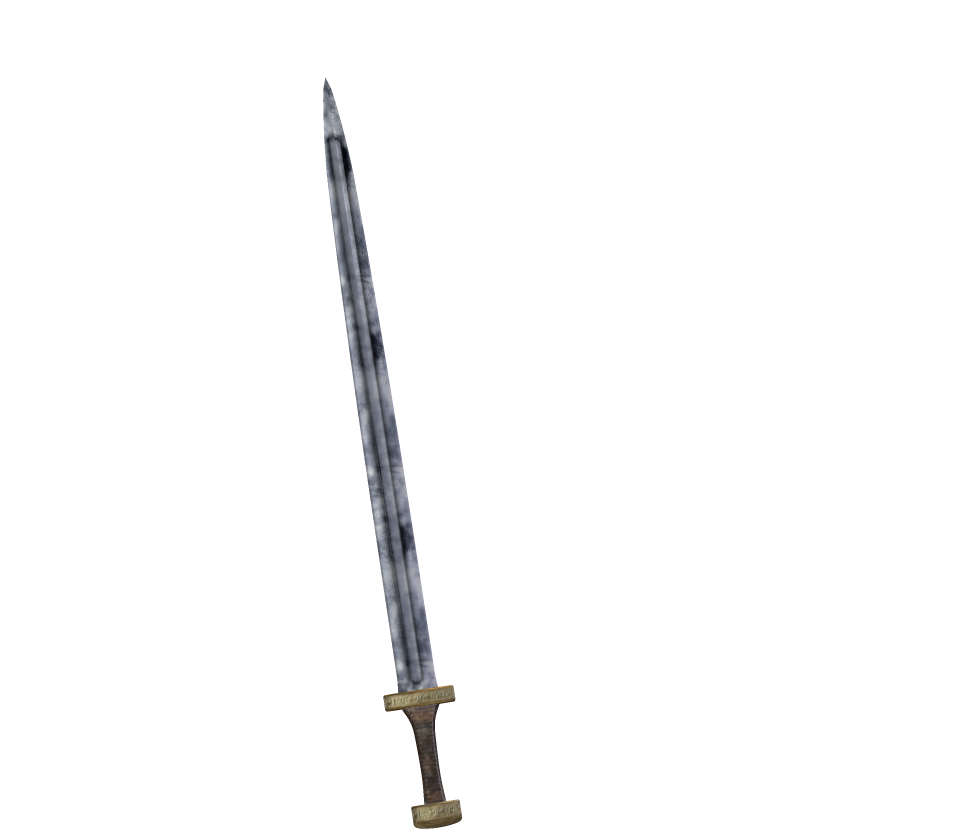
\includegraphics[scale=0.2]{img/sword01.png}
%\end{center}
%\end{figure}


\begin{description}
	\item[Backpack:] It can hold 20 ENC of equipment. 
	\item[Block \& Tackle:] Adds +20\% to Mechanisms tests to make or disarm large traps and makes Engineering tests possible in some circumstances. It requires at least 10m of rope to function. 
	\item[Candle, 1 Hour:]  A candle illuminates a one metre radius. Any wind stronger than a slight breeze will extinguish a candle. 
	\item[Climbing Kit:]  A climbing kit provides a bonus of +20\% to any Athletics skill tests made to climb. 
	\item[Crowbar:] Adds +20\% to brute force Athletics tests. If used as a weapon, it is considered a club (wielded with a –20\% penalty). 
	\item[Healing Kit:] A healing kit is good for five uses (whether the skill test succeeds or fails). 
	\item[Fish Hook:] This item allows a character to use his Natural Lore skill to catch a fish without suffering a penalty on the test. 
	\item[Fishing Kit:] The fishing kit grants a character a +20\% bonus to his Natural Lore test to catch fish. 
	\item[Flint \& Tinder:] A character with flint and tinder can build a fire in one minute under normal conditions without having to roll his Natural Lore skill. 
	\item[Grappling Hook:] It will support the weight of 50 ENC or 50 SIZ, or any combination thereof. 
	\item[Hammer:] If used as a weapon, it is treated as a club (wielded with a –20\% penalty). Hammers may be used on inanimate objects without being destroyed. 
	\item[Lantern:] A lantern provides clear illumination out to a three metre radius. It will burn for two hours on a flask of oil. 
	\item[Lock Picks:] Adds +20\% to Mechanisms tests to unlock a locking device. 
	\item[Mining Pick:] If used as a weapon, it is considered a club (wielded with a –20\% penalty). Mining picks may be used on inanimate objects without being destroyed. 
	\item[Oil, Flask:] A flask of oil is enough to fuel a lantern for two hours or, if broken on the ground and ignited, enough to sustain a small fire for one minute. 
	\item[Quiver:] Quivers can hold up to 30 arrows or crossbow bolts. 
	\item[Rope, 10 Metres:] A standard rope can support the weight of 50 ENC or 50 SIZ, or any combination thereof. 
	\item[Sack, Large:] Able to hold 10 ENC of equipment. 
	\item[Sack, Small:] A small sack can hold 5 ENC of equipment. 
	\item[Scythe:] If used as a weapon, it is considered a polearm (wielded with a –20\% penalty). 
	\item[Slingbag:] It can carry 15 ENC of equipment. 
	\item[Spade:] If used as a weapon, it is considered a club (wielded with a –20\% penalty). 
	\item[Torch, 1 Hour:] It will burn for one hour. A torch illuminates a three metre radius. If used as a weapon, it is considered a club (wielded with a –20\% penalty), except that it does not inflict normal damage – instead, it inflicts 1D4 fire damage and a fumble or critical hit will also extinguish the brand. 
	\item[Waterskin:] A waterskin can hold enough water to sustain an adventurer for two days.
\end{description}

\begin{figure}[h]
\begin{center}
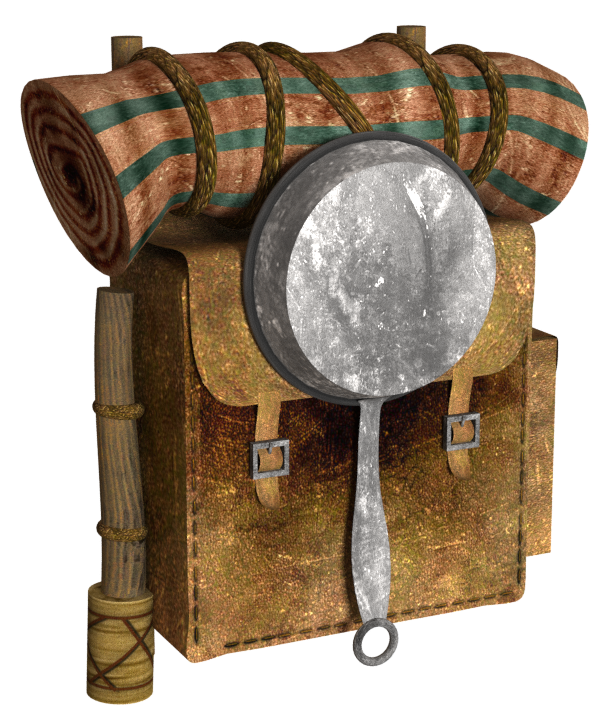
\includegraphics[scale=0.25]{img/Backpack.png}
\end{center}
\end{figure}


\section{Transportation}
\begin{table}[H]
\begin{center}
\caption{Animals and Transportation}
\label{tab:animals-and-transportation}
\begin{rpg-table}[|X|Y|]
	\hline
	\textbf{Animal} & \textbf{Cost}\\
	\hline
	Bison                  & 200 SP\\
	Bull                   & 250 SP\\
	Cart                   & 75 SP\\
	Cat                    & 2 SP\\
	Chariot                & 600 SP\\
	Cow                    & 150 SP\\
	Dog, Domestic          & 2 SP\\
	Dog, Hunting           & 25 SP\\
	Fowl                   & 1 SP\\
	Goat                   & 50 SP\\
	Hawk                   & 400 SP\\
	Horse, Draft           & 400 SP\\
	Horse, Riding          & 350 SP\\
	Horse, Combat Trained  & 500 SP\\
	Mule                   & 125 SP\\
	Ox                     & 200 SP\\
	Pig                    & 50 SP\\
	Saddle and Bridle      & 75 SP\\
	Sheep                  & 30 SP\\
	Travel (by Post-Horse) & 2 SP per kilometre\\
	Travel (by Ship)       & 1 SP per kilometre\\
	Travel (by Wagon)      & 5 SP per kilometre\\
	Wagon                  & 300 SP\\
	\hline
\end{rpg-table}
\end{center}
\end{table}


\section{Food \& Lodging}
\begin{table}[H]
\begin{center}
\caption{Food and Lodging}
\label{tab:food-and-lodging}
\begin{rpg-table}[|X|c|]
	\hline
	\textbf{Animal} & \textbf{Cost}\\
	\hline
	Lodging, Poor                   & 2 CP\\
	Lodging, Average                & 1 SP\\
	Lodging, Superior               & 5 SP\\
	Food and Drink, Poor, 1 Day     & 1 CP\\
	Food and Drink, Average, 1 Day  & 5 CP\\
	Food and Drink, Superior, 1 Day & 2 SP\\
	Trail Rations, 1 Day            & 5 CP\\
	\hline
\end{rpg-table}
\end{center}
\end{table}



\chapter{Combat}
\label{ch:combat}

Fantasy D100 is a swords and sorcery game and, as such, swords will be drawn during epic quests with the aim of spilling blood. Be it for glory, honour, fame or riches, when all else fails violence is the means of achieving these goals. The characters come from worlds that are rife with conflict, where warriors are required to wage wars against evil neighbours, wandering bandits and foul monsters that come out of the wilderness.  

It should be remembered that Fantasy D100 is not a game purely about combat, just as it is not purely about magic. It would not be unusual for whole sessions to pass without any physical violence. However, in time, characters will get involved in dangerous life threatening fights. 

This chapter provides you with a straightforward and direct system for playing out action packed and deadly combat.

\section{Combat is Tough}
Characters that have weapon skills less than 100\% are at the whim of the dice to determine whether or not they land a blow in combat. Anything you do to increase your character’s chances to hit, or hit first, will stand in your favour and make the outcome more certain.

Once you are hit in combat, things start getting messy. Your character has a relatively low number of hit points. In a couple of blows, or one lucky blow, these hit points can easily be reduced to zero, which indicates that the character has died. Make sure your character can dodge, parry or has magical protection. With Major Wounds your character is especially at risk of grievous and permanent harm every time they decide to use violence to solve a problem.

Numbers count. If you are facing off against multiple opponents, even weak and unskilled ones, you are quickly going to run out of attacks and reactions. In practical terms this means that your character may, at best, reduce the number of attackers by one per round, while only being able to protect themselves against one of several incoming attacks. 

Even Masters are vulnerable. A weapon skill over 100\% is no guarantee of survival, as characters can be brought low by a lucky critical hit, or by an opponent who has lured them into an ambush and stacked the odds against them through surprise and careful planning. 

These harsh realities mean that players tend to avoid combats where they do not have a very good chance to win.  Instead of wading into masses of weaker opponents, hoping that lucky dice rolls will see them through, they carefully plan ambushes, where they have the benefit of terrain and supporting soldiers from the local militia that will allow them to wipe out the majority of the enemy before the first proper round of combat. They will any of their talents to boost their damage, chances to hit, or armour and in general try to get an advantage.


\section{Summary of Combat}
\begin{description}
	\item[Work out encounter distance:] The Games Master determines how far away the hostile group is to the player characters, either at Range or Close.

	\item[Drop into Combat time:] Combat is divided into rounds. A single round has a duration of five seconds of time, giving 12 rounds in every minute. During a round every character can perform one action. Combat rounds cycle through the following steps:
	\begin{rpg-list}
	\item Determine Order: At the start of every combat, check each character’s Combat Order,  calculated as $(DEX+INT)/2 + 1D6$. Combat Order is in the character sheet; only the dice needs to be rolled to determine final Combat Order.
	\item Characters Take Action \& Reaction: In a combat round each character gets one Combat Action and one Defensive Reaction. Combat Actions, such as attacks, take place in Combat Order. The character with the highest order will act first, followed by the character with the second-highest order, and so on until the character with the lowest order acts. Reactions, such as parries or dodges, are made during this process as they are needed.
	\item End of Combat Round: Once all eligible characters have acted in the combat round, it is over. If there are characters still engaged in combat with enemies, another combat round begins. 
	\end{rpg-list}
\end{description}

\begin{rpg-examplebox}
For example: Lura has a Combat Order of 15 (13 Dex + 17 Int) and rolled a 3 thus having a final of 18. A Goblin has 13 Combat Order (14 Dex + 11 Int) and rolled a 4 for a total of 17. Thus the Combat Order is Lura acting before the Goblin.
\end{rpg-examplebox}

\section{Encounter Distance}
Not all combats start with the two sides, the players and their opponents, directly facing each other within swords reach.  At the beginning of a combat, or potential combat, the Games Master must determine which of the two distances the encounter starts at.

Close is a range of two metres or less and is the distance at which a character can engage in either Close or Unarmed combat. 

Ranged, beyond two metres up to double the range of the missile weapon a character is holding, is the distance at which the character can engage in ranged combat.  Ranged combat typically happens out in the open countryside where groups of combatants can see each over coming over the horizon or emerging in the distance from old ruined buildings.


\subsection{Some Basic Rules}
\begin{rpg-list}
\item A Combat Round lasts five seconds.

\item You get one Combat Action, usually an attack, and one Defensive Reaction, usually a defensive action, per combat round.

\item You can move your Movement Rate in a Combat Round without losing your Action or Reaction. 

\item You can run twice your Movement Rate in a Combat Round but you may only Dodge as your Reaction.

\item To defend or attack you roll against your Close Combat, Ranged Combat or Unarmed Combat skill depending on the type of weapon you are using.

\item When attacked you can either Parry (use the Close Combat or Unarmed skill) or Dodge as a Reaction.

\item If your character successfully Dodges an attack they take no damage.

\item If your opponent successfully Parries your attack their weapon or shield reduces the damage your attack does.

\item If you successfully hit your opponent takes damage to their hit points equal to 
	Weapon Damage rolled + your Damage Modifier - (Opponent’s Armour Points)
\end{rpg-list}


\section{Combat Actions}
The actions a character may take when it is his turn to act are detailed here. A character can only choose one of the options below each round.

\subsection{Close Combat Actions}
\begin{description}
	\item[Charge:]  If a character can move a minimum of five metres towards his opponent, then he can make a charge. He may move a distance up to - but no more than - twice his Movement Rate.  This must be in a straight line and he must end up adjacent to an enemy.  When the move is complete, a close combat attack may be made against the enemy. If the attack is successful, the character gains a bonus of +1D6 damage. He loses his defensive reaction for the round that he charges on. Characters may not charge uphill and gain the damage bonus.
	\item[Close Combat Attack:]  The character can make a single close combat attack. As well as a normal attack, there are the following special attacks.
		\begin{rpg-list}
		\item All out Attack: The attacker gives up their Reaction for the round but gains a second attack, which happens straight after the first attack. Both attacks are at -20\% due to the loss of skill during this frenzied attack. This type of attack cannot be combined with Great Attack or Disarming Attack.

\item Disarming Attack:  Attacker attacks at -20\% to his weapon skill with the aim of disarming their opponent either of their weapon or shield. If the attack is successful and the opponent fails to parry or dodge, the weapon or shield is thrown 1D6 metres away from the owner. 

\item Great Attack: This attack is made using swords, axes or maces where the attacker has enough room to wind up the weapon for a really forceful blow. The attacker gains a +20\% to attack and automatically does the maximum damage bonus value but loses his reaction for that combat round.
		\end{rpg-list}
	\item[Intimidate/Persuade:]  The character tries to get the other side to surrender or flee. This can either be targeted at a single enemy or a group.  Do an Opposed roll using the character’s Influence vs. the enemies’ Persistence, modified as listed below. Groups roll once using the Persistence of the group leader. If the group leader’s Influence skill is higher than his Persistence, then they may use that skill instead. Apply the following modifiers to the enemy’s skill depending on the state of the enemy.
	\begin{rpg-table}[|c|X|]
		\hline
		+40\% & if the enemy is still at full strength, or has only taken some minor wounds.\\
		+20\% & if the enemy out numbers the player’s side, but have had at least 20\% losses either in numbers or hit points.\\
		-20\% & if the enemy is fewer than the player’s side and has taken some wounds.\\
		-40\% & if the enemy has taken more than half hit points in wounds and/or has seen half his group incapacitated by the players.\\
		\hline
		\multicolumn{2}{|p{\linewidth-4.5mm}|}{Note: these modifiers are not cumulative. Apply the one that best describes the situation.}\\
		\hline
	\end{rpg-table}

If the enemy is at full strength and/or outnumbers the player characters then only a critical roll for Influence vs a failed Persistence roll will make them surrender.  A fumbled Persistence roll will see the enemy suddenly rout.

When the player is attempting the roll they must declare whether they are targeting the whole group or singling out an individual.  The Games Master has the final say on who is targeted and if if attempt is possible at all. 

	\begin{rpg-examplebox}
Rurik is fighting a group of four goblins, one of whom he has already badly wounded while the other three are still at full hit points. 

If he decides to single out the wounded Goblin, then the Goblin’s Persistence roll to resist Rurik’s taunting and the resultant urge to flee will be at -20\%. If he decides to target the whole group, which as a whole is undamaged and outnumbers him, then the Goblins will be at +20\% to their Persistence. 
	\end{rpg-examplebox}

The character need not speak the same language as the opponent they are trying to Influence, but they must be capable of some sort of sign, gesture or body language that the opponent is capable of understanding.

	\item[Set Weapon:]  A character can spend their Action setting the shaft of a weapon, such as a spear or polearm, in the ground in anticipation of a charge from an opponent. When the charge actually comes the character automatically gets an attack at +20\% before the charging character gets their attack. If the character makes any other action or reaction before the charge, the weapon becomes ‘unset’.
\end{description}


\subsubsection{Making Close Combat Attacks}
\begin{rpg-list}
\item Making the Attack: To attack, the player simply rolls 1D100 and compares it to the character’s Close Combat skill which may be modified for the specific situation or special attack being attempted. If a character rolls equal to or lower than his Weapon skill, he has hit his target. If a character rolls greater than his Weapon skill, he has missed his target. 

\item Target Reaction: If the enemy has already reacted this round, or chooses not to React against this attack, then this attack is unopposed. Move straight on to Damage Resolution. If the attack is opposed, the defender makes a Dodge or Parry (see below).

\item Damage Resolution: If the attack is successful, damage is rolled. Each weapon has its own Damage score, to which is added the attacker’s Damage Modifier in order to determine the total damage being dealt. If the defender is armoured then the armour will absorb some of this damage. Reduce the attack’s damage by the armour points (AP) of the defender’s armour. 

\item Damage Application: Apply any remaining damage to the defender’s hit points. 
\end{rpg-list}

\begin{table}
\begin{center}
\caption{Close Combat Situational Modifiers}
\label{tab:close-combat-situational-modifiers}
\begin{rpg-table}[|X|c|]
        \hline
        \textbf{Situation} & \textbf{Skill Modifier}\\
        \hline
        Target is helpless  & Automatic Critical\\
        Target is prone or attacked from behind & +20\%\\
        Attacking or defending while on higher ground or on mount & +20\%\\
        Attacking or defending while prone & -20\%\\
        Attacking or defending while on unstable ground & -20\%\\
        Attacking or defending while underwater & -40\%\\
        Defending while on lower ground or against mounted foe & -20\%\\
        Fighting in partial darkness & -20\%\\
        Fighting in darkness & -40\%\\
        \hline
\end{rpg-table}
\end{center}
\end{table}


\begin{table*}
\begin{center}
\caption{Combat Results}
\label{tab:combat-results}
\begin{rpg-table}[|l|l|X|]
        \hline
        \textbf{Attacker} & \textbf{Defender's Reaction} & \textbf{Result}\\
        \hline
        Fumble   & No need to roll & Attacker funbles.\\
        Failure  & No need to roll & Attacker fails to hit defender.\\
        Success  & Fumble          & Attacker hits, defender takes damage rolled minus armour points and fumbles.\\
        Success  & Failure         & Attacker hits, defender takes damage rolled minus armour points.\\
        Success  & Success         & If dodging defender avoids the attack. If parrying then if attacker’s weapon smaller or equal in size to defender’s weapon all damage avoided. If parrying weapon is a rank smaller half damage, if two ranks smaller then no damage can be avoided.\\
        Success  & Critical        & Defender avoids attack and takes no damage. If parrying the weapon size penalty does not come into it.\\
        Critical & Fumble          & Attacker does maximum damage and ignores defender’s armour. Defender fumbles.\\
        Critical & Failure         & Attacker does maximum damage and ignores defender’s armour.\\
        Critical & Success         & Attacker does maximum damage minus defender’s armour points.\\
        Critical & Critical        & Similar to Success:Success above.\\
        \hline
\end{rpg-table}
\end{center}
\end{table*}


\subsection{Unarmed Combat Actions}
The following are potential actions:
\begin{description}
\item[Unarmed Combat Attack:] The character can make a single Unarmed Combat Attack.
\item[Natural Weapon attack:] Using the characters’s natural weapons be it claw, bite, kick or fist.
\item[Grapple Attack:] The attacker attempts to grab an opponent and an opposed Unarmed Combat Attack is made. If the attacker wins they may chose to inflict pain, immobilise or throw their opponent.
\end{description}

\subsubsection{Making Unarmed Combat Attacks}
Roll against Unarmed Combat skill to determine if the attack is successful. If an Unarmed Attack is parried by a crafted or natural weapon, then the attacker will immediately suffer the rolled damage of the parrying weapon, with no damage modifier. This is in addition to the normal effect of the parry. 

\subsubsection{Natural Weapons}
Natural Weapons such as the teeth and claws of monsters are counted as weapons and not Unarmed Attacks. The damage they deal is listed in the monster’s description. They may parry other Natural Weapons or Unarmed Attacks, but not crafted weapon attacks.

\subsubsection{Grappling}
Grapple Attack is made in the same way as a normal Unarmed or Natural Weapon attack but must be declared as such before any dice are rolled. Should the attacker hit with his grapple attack, no damage is initially caused. Instead, the attacker then opposes his Unarmed Combat Skill to the target’s Unarmed Combat Skill, in a roll similar to an opposed skill test:
\begin{rpg-list}
\item \textbf{Grapple Fails:} The grapple attempt fails and the attack is considered to have missed. 
\item \textbf{Grapple Succeeds:} The two combatants are now grappling and the attacker may immediately follow up on this success by Throwing, Inflicting pain or Immobilise the target.
\end{rpg-list}

\begin{description}
\item[Break Free:] To break out of a grapple, the character makes an opposed Grapple Attack. The characters may only use the Unarmed Combat Skill in this case. If the character succeeds his roll while his opponent fails then the character has succeeded in breaking free and the combatants are no longer grappling, though they will be adjacent.
\item[Immobilise:] While immobilised, enemies are considered helpless. Once per round the defender may attempt to break free.
\item[Inflict Pain:] The grappler inflicts damage of 1D4 + damage modifiers.  Armour does not help. Once per round the defender may attempt to break free or may attempt to turn the tables on their attacker by counter grappling.
\item[Throw:] The opponent is thrown 2 metres and suffers 1D4 damage. Armour does not help. The grapple ends in this case.
\end{description}


\subsection{Ranged Combat Actions}

The following are potential actions:
\begin{description}
\item[Ranged Combat Attack:] The character can make a single ranged combat attack. As well as a normal attack, there is the following special attacks.
\item[Aim:] Every round spent aiming adds a +20\% bonus to the character’s Ranged Combat skill. This bonus only applies to the first attack the character makes with the weapon, which must be fired at the target being aimed at. A character can aim a maximum of 2 rounds and can take no other Reaction while aiming without losing the aim bonus.
\end{description}

\subsubsection{Throwing Close Combat Weapons}
If a close combat weapon that isn’t designed to be thrown is hurled at an enemy then it has a range of 8m and suffers a penalty to the attack equal to its ENC x 10. Ranged Combat skill is used. 

\subsubsection{Using Ranged Weapons}
All ranged attacks are handled in same manner as close combat attacks, with the following exceptions: 
\begin{description}
\item[Charge:] Ranged attacks may not be used as part of a charge.
\item[Loading Ranged Weapons:] Most ranged weapons only take a single combat round to ready. Others take more than one combat round to reload. See weapon description in the equipment chapter. 
\item[Range:] A target within the weapon’s range may be attacked without penalty. A target within double the weapon’s range may be attacked, but the attacker’s weapon skill is halved before other modifiers are applied. Attacks cannot be made at a distance beyond twice/double the weapon’s range.
\item[Dodging and Parrying:] The target may attempt to Parry or Dodge a hand thrown ranged attack at -20\% but may not normally Dodge or Parry ranged missile weapons (such as Bows and Crossbow fire). Shield-carrying characters may Parry hand thrown missile weapons with no penalty.
\item[Disarming:] A character may not attempt to disarm targets with ranged attacks, nor may he attempt to strike a target’s weapon or shield.
\end{description}

\subsubsection{Cover}
Cover affects both ranged and close combat attacks. For missile attacks the defender benefits from the best of the shield modifier in the table above and the cover modifier below.

\begin{description}
	\item[Partial cover (-20\%):] For example a low wall that leaves only head and torso exposed.
	\item[Very good cover (-40\%):] For example Defender on a castle wall, firing from protected battlements.
	\item[Virtual total cover (-80\%):] For example castle wall with arrow slits for defenders to shot through.
\end{description}


\begin{table}
\begin{center}
\caption{Ranged Attack Situational Modifiers}
\label{tab:ranged-attack-situational-modifiers}
	\begin{rpg-table}[|p{5cm}|Y|]
	\hline
        \textbf{Situation} & \textbf{Skill Modifier}\\
	\hline
	\multicolumn{2}{|p{\linewidth-4.5mm}|}{Wind$^{1}$}\\
	\hline
        High wind    & -20\%\\
        Fierce wind  & -60\%\\
        Hurricane    & Attack automatically fails\\
	\hline
	\multicolumn{2}{|p{\linewidth-4.5mm}|}{Target Movement$^{1}$}\\
	\hline
        Target has moved 10m or more since attacker's last Combat Action  & -20\%\\
        Target has moved 30m or more since attacker's last Combat Action  & -40\%\\
	\hline
	\multicolumn{2}{|p{\linewidth-4.5mm}|}{Target Visibility$^{1}$}\\
	\hline
        Target obscured by smoke, mist or is in partial darkness          & -20\%\\
        Target obscured by thick smoke, fog or is in darkness             & -40\%\\
        Target is above SIZ 20                                            & +20\%\\
	\hline
	\multicolumn{2}{|p{\linewidth-4.5mm}|}{Target Condition$^{1}$}\\
	\hline
        Target is helpless                                                & +40\%\\
        Target is prone                                                   & -20\%\\
	\hline
	\multicolumn{2}{|p{\linewidth-4.5mm}|}{Attacker Condition$^{2}$}\\
	\hline
        Attacker is prone                                                 & -40\%\\
	Attacker is underwater$^{3}$                                      & -20\%\\
	Attacker is on unstable ground                                    & -20\%\\
	Attacker is blinded                                               & -40\%\\
	\hline
	\multicolumn{2}{|p{\linewidth-4.5mm}|}{1. Modifiers within these sections are not cumulative. However, modifiers from different sections are cumulative. Therefore, shooting at a target within a mist that has moved more than 10m since the attacker’s last Combat Action imparts a –40\% penalty.}\\
	\multicolumn{2}{|p{\linewidth-4.5mm}|}{2. Attacker condition modifiers are cumulative.}\\
	\multicolumn{2}{|p{\linewidth-4.5mm}|}{3. Only crossbows may be used underwater.}\\
	\cline{1-2}
\end{rpg-table}
\end{center}
\end{table}




\part{Disciplines and Powers}
\chapter{Disciplines}
\label{ch:disciplines}

\section{Introduction}
Disciplines provide a wide variety of different extraordinary and/or supernatural options to embelish your campaigns. You can pick and choose what disciplines make more sense to your campaign or you can even come up with your own.

Common in all disciplines is their dependence on certain characteristics. Most use POW and spend Power Points one way or another.

\section{Power}

\subsection{Regaining Power Points}
Using Power Points is a draining and exhausting activity that requires a major effort from which the body needs to recover. Power Points regenerate once the character fully rests, either by sitting down and taking it very easy or by having a good nights sleep. 

For every two hour period that a character rests they regain Power Points equal to a quarter of their POW total.  

\begin{rpg-examplebox}
Rurik, with a POW of 8, takes two hours of rest to regain two Power Points, four hours to regain four Power Points, six hours to regain six Power Points and eight hours to regain the full eight Power Points. 
\end{rpg-examplebox}

Basically, if the character has a comfortable uninterrupted sleep of eight hours they will regain their full power points. Characters may never exceed their original Power Point total by resting.

\subsection{Zero Power Points}
A character who is reduced to zero Power Points falls unconscious until he has regained one Power Point.

\subsection{Beyond Maximum}
There are ways of surpassing the maximum number of Power Points available to characters by using some of the supernatural powers described in the disciplines found in the following chapters. For examples practitioners of the Magic discipline can have access to additional pools of Power Points, via bound Magic Spirits (see Call Spirit spell) and magic items that act as Power Point Stores (see Create Power Point Store spell). However, these pools regenerate, if at all, independently of the character’s natural rate. Experienced Magic users could potentially have several Power Point stores and bound Magic Spirits at their disposal, which allows them to cast many of their spells without using their own precious pool of Power Points.


\chapter{Battle}
\label{ch:battle}

The Battle Discipline represents years of advanced traning in combat techniques. It enables warriors to reach an understanding of the flow of battle to such a degree that he can gain advantages over their opponents. Some times that is forcing an opponent to leave an opening or positioning themselves in such a way to avoid harm. Other times it enables unprecedented focus and calmness in the midst of battle enabling precise and calculated blows.


\section{Spot Rules}

\subsection{Learning Battle}
Characters learn Battle from other characters who know the practice. They need to have at least 51\% to a combat skill and spend two Improvement Points to get access to the Battle discipline. Each technique is learnt separately.

%With enough perseverance a character can practice and learn this Discipline by themselves but that will cost them double the Improvement Points normally required.

\subsection{Learning Techniques}
Characters learn Battle Techniques from other characters who know the appropriate techniques. Learning techniques costs one Improvement Point per Magnitude point. 
%If a character knows a technique at a lower Magnitude, they only have to pay the difference in Improvement Points to gain the technique at a higher Magnitude.

The maximum number of Battle Techniques a character can learn is INT/2.

%\begin{rpg-examplebox}
%Bors found a master that is willing to teach him Combat Mastery. He trains with him for some time and manages to learn the new technique (by spending three improvement points).
%%%Bors already knows Weapon Mastery at 1 Magnitude. He wants to learn Weapon Mastery 2, so he must spend only one Improvement Point to gain the technique at that Magnitude.
%\end{rpg-examplebox}

Battle Techniques can be learnt from a number of sources. The most typical is from military academies but it can also be from the lone retired veteran. 

In each case the player character must be in good standing with the teacher before they will teach them a technique. If the teacher is indifferent to the player character to start with then they will first need to undertake some kind of service, which can be the focus of an adventure.

\begin{rpg-titlebox}{Optional: Self-taught}
With enough perseverance a character can practice and learn new Battle Techniques by themselves but that will cost them double the Improvement Points normally required.
\end{rpg-titlebox}

\subsection{Using Techniques}
A character can use a technique freely as part of a combat action or reaction. Only a single Battle Technique can be used per combat round. Any Battle Technique needs to be declared before the appropriate dice is rolled.

Applying a Battle Technique is always successful but you have to spend a number of Power Points equal to the Magnitude of the technique.


\subsection{Techniques Traits}
Unless otherwise stated all Techniques have the following traits.

\begin{rpg-list}
\item Are instant and apply only for the action or reaction that are rolled for.
\item Can not be used in combination with special attacks like Great Attack, Disarming Attack, Aim, etc.
\item Are Non-Variable; they can only be used at the specified Magnitude.
\end{rpg-list}

%Other traits used by techniques are detailed below. 
%\begin{description}
%	\item[Single-Attack:] Applies to a single attack.
%	\item[Combat Round:] Applies for the whole combat round (for that character)
%	\item[Non-Variable:] The technique may only be used at the stated Magnitude.
%\end{description}

\section{Techniques}
The battle techniques can improve various aspects of combat. Some are improved versions of existing manoeuvres, like Improved Disarm, while other are new, like Defensive Stance. These manoeuvres make more sense to acquire for combat experts since they will already have a high skill (which is harder to increase).

\begin{center}
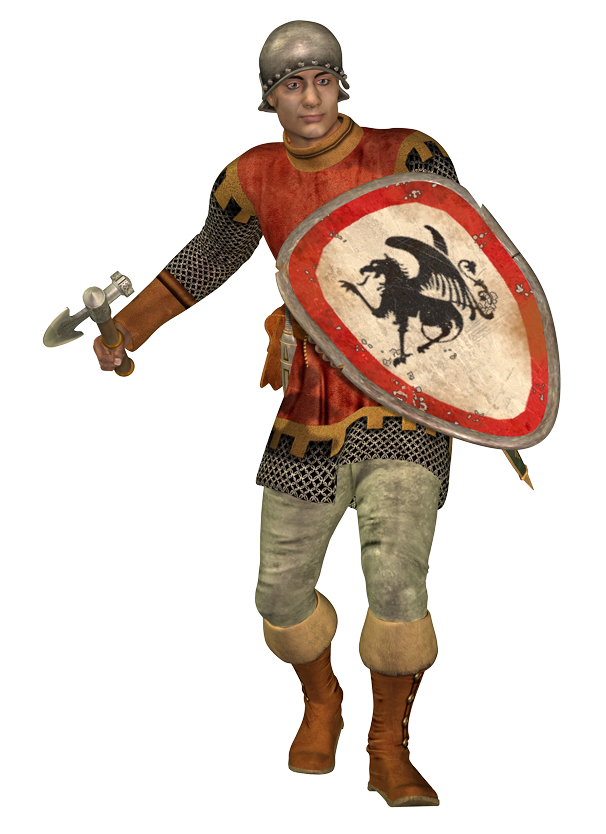
\includegraphics[scale=0.27]{img/colored/adventurer2.png}
\end{center}


\begin{table*}
\begin{center}
\caption{Battle Techniques}
\label{tab:battle-techniques}
\begin{rpg-table}[|l|c|X|]
        \hline
	\textbf{Technique} & \textbf{Magnitude} & \textbf{Effect}\\
	Awareness & 3 &  When the warrior is aware of an opponent the latter cannot gain a flanking bonus for three combat rounds.\\
	Combat Focus & 2 &  Allows a warrior to make a close combat attack with a +20\% bonus.\\
	Combat Mastery & 3 &  Allows a warrior to make a close combat attack with a +20\% bonus and +2 damage. If Combat Focus is already known it can be substituted with this technique with one Improvement Point. \\
	Confuse & 2 &  Can only be used for an attack action and forces the opponent's parry or dodge to be at -20\%.\\
	Deadly Aim & 3 &  Allows a warrior to make a ranged attack with a +20\% and +2 damage.\\
	Defensive Stance & 4 &  When the warrior is wielding a shield their effective Armor Points is increased by one for four combat rounds.\\
	Extra Reaction   & 3 &  The warrior gains an extra reaction in this round with a -20\% modifier.\\
	Impr. Combat Order & 2 &  Allows a warrior to react faster (needs to declare before Combat Order rolls). It provides +4 to Combat Order.\\% and +20\% to dodge or DEX-based Athletics tests.\\
	Impr. Aim & 2 &  The attack is similar to the Aim special attack but is immediate.\\
	Impr. All Out Attack & 4 &  The attack is similar to the All Out special attack but without losing the reaction.\\
	Impr. Disarm & 2 &  The attack is similar to the Disarm special attack but without the penalty.\\
	Impr. Trip   & 2 &  The attack is similar to the Trip special attack but without the penalty.\\
	Impr. Great Attack & 4 &  Allows a warrior to make a Great Attack without losing their reaction.\\
	Impr. Intimidate & 2 &  The warrior's intimidate (Influence) is increased by 20\%.\\
	Impr. Knock-Back & 2 &  The attack is similar to the Knock-Back special attack but without the penalty.\\
	Impr. Knockout & 2 &  The attack is similar to the Knockout special attack but at +20\% (negating the off-hand penalty).\\
	Twin Attack & 2 &  The attack is similar to the All Out special attack but with no penalty for the first attack.\\
	Twin Missile & 4 &  Allows a warrior to make an additional single ranged attack action at -20\% in quick succession.\\
	Unarmed Fast Attack & 2 &  When unarmed a warrior can make an additional unarmed attack at -20\% in quick succession.\\
	Unarmed Focus & 2 &  Allows a warrior to make an unarmed attack with a +20\% bonus.\\
	Unarmed Mastery & 3 &  Allows a warrior to make an unarmed attack with a +20\% bonus and +2 damage. If Unarmed Focus is already known it can be substituted with this technique with one Improvement Point.\\
        \hline
\end{rpg-table}
\end{center}
\end{table*}


\chapter{Magic}
\label{ch:magic}

This discipline represents common magic or hedge magic. It is the typical type of magic that most campaigns will have. Magic is generally of a practical nature, meant to address battle or the common ills of the community: healing the sick, bringing love or luck, driving away evil forces, finding lost items, reading omens and so on. 


\section{Spot Rules}

\subsection{Learning Magic}
Magic Casting is treated as a skill. The base chance for Magic Casting is POWx3. Spells are learnt separately, but the Magic Casting skill determines the success for casting all Magic spells. Characters learn Magic from other characters who know the practice. It costs four Improvement Points to get access to the Magic discipline.

\subsection{Learning Spells}
Characters learn Magic spells from other characters who know the appropriate spells. Learning spells costs one Improvement Point per Magnitude point. If a character knows a spell at a lower Magnitude, they only have to pay the difference in Improvement Points to gain the spell at a higher Magnitude.

\begin{rpg-examplebox}
Adjin already knows Animal Whisperer at 2 Magnitude. He wants to learn Animal Whisperer 3, so he must only spend one Improvement Point to gain the spell at that Magnitude.
\end{rpg-examplebox}

Magic can be learnt from a number of sources. The most typical is from some kind of school of magic appropriate for the campaign or from remote hermits and otherworldly Shamans who commune with the Spirit World and learn it's secrets. In some cases, it can be learnt from local priests who teach Magic associated with their gods’ mythological exploits.

In each case the player character must be in good standing with the teacher before they will teach them the spell. If the teacher is indifferent to the player character to start with then they will first need to undertake some kind of service, which can be the focus of a Quest.

\subsection{Casting Spells}
A character must be able to move his hands to make gestures and be able to chant in order to cast a spell and must be able to see his target. 

When the character is casting a spell under duress, such as in the midst of combat, they must pass a Magic Casting test to successfully cast the spell. In this regard Magic is like any other skill. If the character is relaxed and has all the time in the world then no casting test is needed, the spell is automatically cast.

The result of the Magic casting test depends on its success:
\begin{description}
	\item[Success:] A number of Power Points are deducted from the spellcaster’s total, equal to the Magnitude of the spell. The spell then takes effect.
	\item[Failure:] The spell does not take effect and the character loses one Power Point.
	\item[Critical:] The caster has been able to control the flow of the magic particularly effectively. The character loses one Power Point instead of the normal cost of the spell.
	\item[Fumble:] The caster has been unable to control the flow of the Magic. Rather than losing a single Power Point for failing to cast the spell, the caster loses a number of Power Points equal to its Magnitude. 
\end{description}

\begin{figure}[h]
\begin{center}
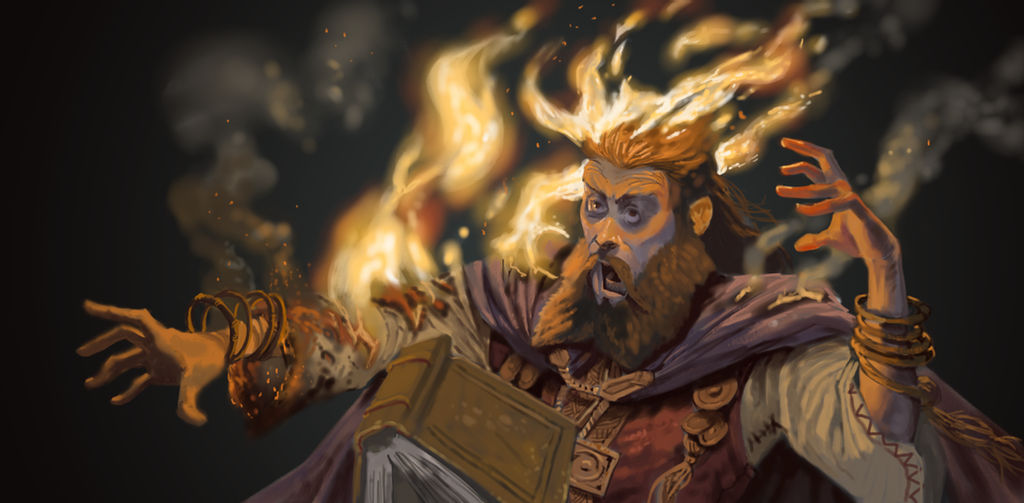
\includegraphics[scale=0.23]{img/backfire_by_ncorva.jpg}
\end{center}
\end{figure}


\subsubsection{Casting Time}
No other action may be taken whilst casting a spell, though the character may slowly walk up to half their Movement while spell casting. %All spells take one combat round to cast.

Casting begins at the start of the combat round and a spell’s effect happens on the caster’s INT, instead of DEX, (which is used for close combat).  

Distractions, or attacks on the caster as he casts, will automatically ruin the spell, unless the caster successfully passes a Persistence test, thereby maintaining concentration on the spell. Examples of distraction include blinding, disarming, or wounding the caster.

\subsubsection{Dismissing Spells}
In a single Combat Round, a caster can dismiss any Permanent spell(s) he has cast, as a free action. Ceasing to cast a Concentration spell is immediate and not an action. 


\subsection{Spell Traits}
Unless otherwise stated all Magic spells have the following traits.

\begin{rpg-list}
\item They have Variable Magnitude. This means that the Magnitude of the spell starts from the stated Magnitude and then can be cast at a higher Magnitude, if the caster knows it, giving an increase in the effect of the spell. The maximum Magnitude that a caster can learn is equal to their POW divided by 3.
\item Base Magnitude is one. 
\item Range is equal to the caster’s POWx3 in metres.
\item All spells, unless noted, have a Duration of ten minutes.
\end{rpg-list}

Other traits used by spells are detailed below. 
\begin{description}
	\item[Area (X):] The spell affects all targets within a radius specified in metres. 
	\item[Concentration:] The spell’s effects will remain in place so long as the character continues to concentrate on it. Concentrating on a spell is functionally identical to casting the spell, requiring the caster to continue to chant and ignore distractions. 
	\item[Instant:] The spell’s effects take place instantly. The spell itself then disappears. 
	\item[Magnitude (X):] The strength and power of the spell. Also the minimum number of Power Points required to cast it. 
	\item[Non-Variable:] The spell may only be cast at the stated Magnitude.
	\item[Permanent:] The spell’s effects remain in place until they are dispelled or dismissed. 
	\item[Resist (Dodge/Persistence/Resilience):] The spell’s intended effects do not succeed automatically. The target may make a Dodge, Persistence or Resilience test (as specified by the spell) in order to avoid the effect of the spell entirely. Note that Resist (Dodge) spells require the target to be able to use Reactions in order to Dodge. In the case of Area spells, the Resist (Dodge) trait requires the target to dive in order to mitigate the spell’s effect. 
	\item[Touch:] Touch spells require the character to actually touch his target for the spell to take effect, using a Unarmed skill test to make contact. The caster must remain in physical contact with the target for the entire casting.
	\item[Trigger:] The spell will lie dormant until an event stated in the description takes place. The spell then takes effect and is expended.
\end{description}

\section{Spells}

\begin{rpg-spell}
{Animal Whisperer}
{Magnitude 2, Non-Variable, Touch}

The caster whispers into the ear of a distressed animal, calming it. If the distressed animal is under the influence of a spell such as Fear or Scare, then its gets another Persistence test to shake off the effect of the spell.
\end{rpg-spell}


\begin{rpg-spell}
{Avoidance}
{Instant, Trigger}

This spell lies dormant until the recipient is attacked. Then, after the normal reaction of the recipient, it fires off allowing the recipient to Dodge a number of times equal to the spell’s Magnitude. Once triggered, all the extra Dodge reactions are valid for that round only.
\end{rpg-spell}


\begin{rpg-spell}
{Babel}
{Magnitude 2, Non-Variable, Resist (Persistence)}

If this spell is successful, it garbles the language of the affected creature. The target can still think and, for the most part, act normally, but anything it says comes out as gibberish. Thus, a commanding officer would be unable to give orders to his men and a spellcaster would be unable to cast spells.
\end{rpg-spell}


\begin{rpg-spell}
{Bearing Witness}
{Instant}

This spell grants the caster a +10\% bonus per point of Magnitude to their next Skill Test they make to discover lies, secrets or hidden objects. It does not stack with any other spell-effect bonuses.
\end{rpg-spell}


\begin{rpg-spell}
{Beast Call}
{Magnitude 2, Non-Variable, Instant, Resist (Resilience)}

The Beast Call serves to attract an animal within range. When the spell is cast, it affects a targeted creature with a fixed INT of 7 or less. If it fails to resist, the creature will be naturally drawn to the place where the spell is cast, whereupon the spell effect terminates. Any barrier, immediate threat, or counter control, also ends the effects of the spell, leaving the creature to react naturally. 

For example, the Beast Call spell might cause a horse to turn and walk towards the spell, but a single yank of its reins by the rider would end the spell’s effect. This spell is a potent aid to hunters and herders.
\end{rpg-spell}


\begin{figure*}
\begin{center}
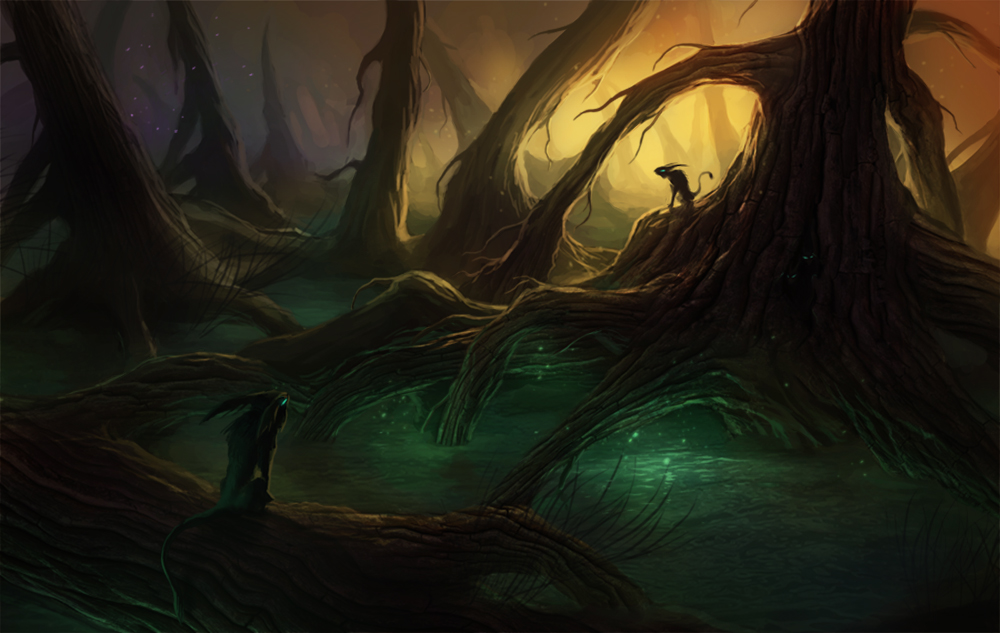
\includegraphics[scale=2.1]{img/mystical_forest_by_sirend.jpg}
\end{center}
\end{figure*}


\begin{rpg-spell}
{Befuddle}
{Magnitude 2, Non-Variable, Resist (Persistence)}

The affected target may not cast spells and may only take non-offensive actions. The target may run if it so chooses and may dodge and parry normally in combat, though it may not make any attacks unless it is attacked first. 

This spell is effective against humanoids and natural creatures. Other creatures (such as spirits or magical beasts like dragons) are not affected by this spell. 
\end{rpg-spell}


\begin{rpg-spell}
{Call Spirit}
{Magnitude 3, Non-Variable, Resist (Persistence)}

This spell is used to summon a single spirit of a given type from the Spirit World to do the bidding of the caster. Unless combined with a Binding attempt (see Spirit Binding Ritual spell below), a spirit that fails a Persistance roll must perform one action, within its power, for the caster after which it returns to the Spirit World.

The spirit resists the call by using its Persistence. If it succeeds it can return to the Spirit World. 

\begin{rpg-list}
\item Disease spirits, inflict disease upon the possessed victim.
\item Passion (Fear/Madness/Pain) these spirits work upon the passions of a victim and cause mental debilitation and distress.
\item Healing spirits, can be used to heal wounds and drive out possessing Disease spirits.
\item Magic spirits, know spells and have power points that the caller may use.
\item Guardian Spirits, protect a location for the casters POW in minutes.
\item Ancestor Spirit, can pass on one piece of wisdom or increase one skill for the spells duration.
\end{rpg-list}
\end{rpg-spell}

 
\begin{rpg-spell}
{Block Sense (Sense)}
{Magnitude 3, Non-Variable, Resist (Persistence)}

This spell will Blind, Deafen, Bland taste or Numb touch on a failed resistance roll for the duration of the spell.
\end{rpg-spell}


\begin{rpg-spell}
{Care}
{Magnitude 2, Non-Variable, Touch}

This charm places the recipient under the care of the caster. If the caster has any active Protection or Countermagic spells, the Cared for character also benefits from the effects of these spells.
\end{rpg-spell}

\begin{rpg-spell}
{Clear Path}
{Touch}

This spell allows the caster to move through even the most tangled, thorny brush, as if they were on an open road. For each additional point of Magnitude, they may bring one person with him. 
\end{rpg-spell}


\begin{rpg-spell}
{Coordination}
{Touch}

For every point of Magnitude, the target’s combat order increases by +2, whether casting spells or fighting and 10\% is added to Dodge or DEX-based Athletics tests. 
\end{rpg-spell}


\begin{rpg-spell}
{Counter-Attack}
{Magnitude 2, Non-Variable, Trigger}

This spell lies dormant until the recipient is attacked. Then, after the normal defensive reaction of the recipient, it fires off, allowing the recipient to follow up with a counter attack. The counter attack is an additional action, on top of the recipient’s normal attacking action.
\end{rpg-spell}


\begin{rpg-spell}
{Counter-Defense}
{Magnitude 2, Non-Variable, Trigger}

This spell lies dormant until the recipient is successfully attacked. Then after the normal reaction of the recipient, it fires off allowing the recipient an extra defence.
\end{rpg-spell}



\begin{rpg-spell}
{Countermagic}
{Instant}

Countermagic is only ever used as a Reaction, and only when another spell is cast within Countermagic’s Range that the character wishes to counter. A successful Countermagic disrupts the other spell and nullifies it. As long as Countermagic’s Magnitude equals or exceeds the target spell’s Magnitude, the target spell is countered.
\end{rpg-spell}


\begin{rpg-spell}
{Create Charms}
{Permanent}

A charm is a physical item that stores one or more Magic spells. A charm could be a necklace that holds a Befuddle 4 spell, a shield etched with runes that holds a Countermagic 2 spell, or even a sheet of paper with a poem written on it that, when held against the skin, provides a Protection 1 spell.

\begin{rpg-list}
\item To create a charm a character must possess both the spell they wish to store and Create Charm at the same Magnitude.
\item The item into which the charm is to be cast must be prepared and in contact with the caster for the length of the casting.
\item If the caster spends one Improvement Point at the time of creation the spell is reusable. Otherwise once the spell is cast the Charm is dispelled. A spell stored in a Charm is used like any other spell that the possessor knows. It uses the wielder’s Magic Casting skill and is powered by the wielder’s Power Points.
\item If the caster spends three Improvement Points per Magnitude at the time of creation the spell within the Charm is reusable, once per day (1/day), without requiring a Magic Casting skill or any Power. It can be activated as an Action. If the Create Charms spell is cast again then it becomes 2/day, and so on. Not all spells can be stored this way and the Gamemaster has the final say.
\item If the caster spends ten Improvement Points per Magnitude at the time of creation the spell within the Charm is always active, without requiring a Magic Casting skill or any Power. These are the most powerful charms. Not all spells can be stored this way and the Gamemaster has the final say.
\item The time taken to create a single-use Charm is one hour per point of Magnitude of the spell being stored; Reusable Charms take three hours per point of Magnitude to create.
\item Charms are mundane items in their own right and if the item is broken the Charm is dispelled.
\end{rpg-list}
\end{rpg-spell}


\begin{rpg-spell}
{Create Power Point Store}
{Permanent}

This spell allows the caster to create an item which has Power Point storing capabilities. This allows the owner to have a pool of Power Points in addition to their own.

Typically crystals are used, due to their physical toughness, in game terms treat them as unbreakable. This also applies to charms, such as a sword with Weapon Enhancement 2 stored in it, to provide a pool of power points to cast the spell from.

Power Point stores take one hour per Power Point stored in them to create. For each Magnitude, one Power Point can be stored.

Unless one Improvement Point is spent when they are created they are non-reusable. Once the Power Points are used the item loses its ability to store Power Points. If the Improvement Point is spent the item then becomes reusable. Once all the Power Points are used, the item can be refilled instantly from the user’s own Power Points.

The caster must fill the item with their own Power Points as part of the spell. The amount of Power Points put into the item at the time of casting becomes the maximum that can be put into the item. This maximum can not be increased after the spell is cast.

If the item is destroyed the Power Points are released harmlessly into the surrounding area.
\end{rpg-spell}


\begin{rpg-spell}
{Create Potions}
{Permanent}

Potions are liquids that store one or more Magic spells. The Magnitude of the Create Potion spell needs to equal or exceed the highest Magnitude of the spell being stored into the potion.

\begin{rpg-list}
\item All potions are one use. They must be drunk in one swift gulp to work. 
\item The potion automatically works and doesn’t incur a cost in power points to the person who is drinking it. 
\item The potion costs the enchanter Power Points. They must know the spell at the Magnitude enchanting at, with the Power Points of the spell being put into the potion. 
\item There is an associated cost of 10 Gold Pieces per Magnitude. 
\item To make the potion, the enchanter must roll successfully against Magic Casting for each spell being placed in the potion and against Lore (Potion Making). If they fail the potion is ruined and they lose the cost of the ingredients. 
\item Potions take one hour per point of Magnitude of spell(s) stored to create. 
\item A potion must be stored in an air tight container, or it evaporates, losing one point of Magnitude per week. 
\end{rpg-list}
\end{rpg-spell}


\begin{rpg-spell}
{Cushion Fall}
{}

Each point of Magnitude of this spell eliminates one dice of falling damage for the recipient.
\end{rpg-spell}


\begin{rpg-spell}
{Darkwall}
{Area 5, Magnitude 2, Non-Variable}

Light sources within a Darkwall area shed no light and normal sight ceases to function. Other senses such as a bat’s sonar function normally. 
The caster may move the Darkwall 15 metres per Combat Round. If this option is chosen, the spell gains the Concentration trait. 
\end{rpg-spell}


\begin{rpg-spell}
{Demoralise}
{Magnitude 2, Non-Variable, Resist (Persistence)}

This spell creates doubt and uncertainty into the very heart and soul of the target. The target of this spell has all Weapon skills halved and may not cast offensive spells. If this spell takes effect before combat begins, the target will try to avoid fighting and will either run or surrender. The effects of this spell are automatically cancelled by the Fanaticism spell and vice versa. 
\end{rpg-spell}


\begin{rpg-spell}
{Detext (X)}
{Magnitude 1, Non-Variable, Concentration}

This covers a family of spells that all operate in a similar fashion, allowing the caster to locate the closest target of the spell within its range. This effect is stopped by a thick substance, such as metal, earth or stone, if it is at least one metre thick. It is also blocked by Countermagic, though the caster will know the target is somewhere within range (though not its precise location) and that it is being protected by Countermagic. The separate Detect spells are listed below and each must be learned separately.

\begin{rpg-list}
\item Detect Enemy: Gives the location of the nearest creatures, that intend to harm the caster. 
\item Detect Magic: Gives the location of the nearest magic item, magical creature or active spell. 
\item Detect Species: Each Detect Species spell will give the location of the nearest creature of the specified species. Examples of this spell include Detect Goblin, Detect Rhino and Detect Elf. 
\item Detect Substance: Each Detect Substance spell will give the location of the nearest substance of the specified type. Examples of this spell include Detect Coal, Detect Gold and Detect Wood. 
\end{rpg-list}
\end{rpg-spell}


\begin{rpg-spell}
{Dispel Magic}
{Instant}

This spell will attack and eliminate other spells. Dispel Magic will eliminate a combined Magnitude of spells equal to its own Magnitude, starting with the most powerful affecting the target. If it fails to eliminate any spell (because the spell’s Magnitude is too high), then its effects immediately end and no more spells will be eliminated. A spell cannot be partially eliminated, so a target under the effects of a spell whose Magnitude is higher than that of Dispel Magic will not have any spells currently affecting it eliminated. 
\end{rpg-spell}


\begin{rpg-spell}
{Disruption}
{Instant, Resist (Resilience)}

Disruption literally pulls a target’s body apart. The target will suffer 1D4 points of damage per point of Magnitude, ignoring any Armour Points. 
\end{rpg-spell}


\begin{rpg-spell}
{Dragon Fire}
{Magnitude 2, Non-Variable, Instant, Resist (Dodge)}

With this spell, the caster throws a stream of fire at his target. If the fire is not dodged, it inflicts 1D10 points of heat damage. Armour Points are effective against this damage and it counts as both magical and fire damage.
\end{rpg-spell}


\begin{rpg-spell}
{Drive Out Spirit}
{Instant, Resist (Spirit Combat)}

This spell excommunicates a spirit that is either dominantly or covertly possessing a character (see Chapter \ref{ch:shamanism} for details on possession type). The spirit resists eviction from its host using its Spirit Combat skill, with a penalty of -10\% for every Magnitude point of the spell. If the spirit is reduced to 0 Power Points it is driven back to the Spirit World. This spell allows the caster to initiate Spirit Combat even if they are not a Shaman, but only against a possessing spirit, not discorporate ones. It is possible to combine this spell with Spirit Bane and Spirit Shield, but not Spirit Binding.
\end{rpg-spell}


\begin{rpg-spell}
{Dull Weapon}
{}

This spell can be cast on any weapon. For every point of Magnitude it reduces the damage dealt by the target weapon by one. 
\end{rpg-spell}


\begin{rpg-spell}
{Enhance Skill (X)}
{Instant}

Like Detect (X), this includes a number of different spells, each of which affects a different non-combat skill. For each point of Magnitude, the recipient gains +10\% to any skill test using the Enhanced skill.  Alternatively, for each additional point of Magnitude of the spell, the caster can affect one more target. The bonuses and targets can be split as necessary, providing each bonus is in multiples of 10\% and the total of bonuses equals the spells Magnitude x 10\%.

For example, Adjin may have Enhance Skill (Deception) 5.  He could cast it all on himself to give a whopping +50\% to his Deception, or could cast it on himself and an ally, giving himself +30\% and his ally +20\%. If in a larger group, he could even cast it on 5 allies, each of whom would gains +10\% to their Deception skill.

The most common spells of this type are:
\begin{rpg-list}
\item Enhance Skill (Deception), often used by thieves.
\item Enhance Skill (Trade), used by merchants.
\item Enhance Skill (Influence), used by lawyers, con-artists and officers.
\item Enhance Skill (Resilience), used by warriors.
\item Enhance Skill (Persistence) used by magicians.
\end{rpg-list}

These spells are sometimes called by other names, such as “Cover of Night” or “Shadowstealth” (for Enhance Deception), “Golden Tongue” (for Enhance Influence or Trade), or “Toughen” (for Enhance Resilience).
\end{rpg-spell}


\begin{rpg-spell}
{Extinguish}
{Instant}

This spell instantly puts out fires. At Magnitude 1 it can extinguish a Flame, Magnitude 2 a Small Fire, Magnitude 3 a Large Fire and Magnitude 4 will put out an Inferno.
\end{rpg-spell}


\begin{rpg-spell}
{Total Awareness}
{Magnitude 2, Non-Variable}

This spell grants the recipient awareness as if they had physically got eyes in the back of their head for the duration of the spell. This allows them to make Perception rolls, and be aware of others behind them as they are with senses in front of them.
\end{rpg-spell}


\begin{rpg-spell}
{Fanaticism}
{Magnitude 2, Non-Variable}

The target of this spell will have close combat and unarmed combat skills increased by +20\% but may not attempt to parry, dodge or cast spells. Also for the duration of the spell the target has a +40\% bonus to any Persistence test related to Morale. The effects of this spell are automatically cancelled by the Demoralise spell and vice versa.
\end{rpg-spell}


\begin{rpg-spell}
{Fire Missile}
{Magnitude 2, Non-Variable, Touch, Trigger}

Casting this spell on a missile will cause it to burst into flame when it is fired/thrown and strikes a target. When it hits a target, the missile will deal 1D10 points of magical fire damage instead of its normal damage. Since Fire Missile does magical damage, it affects creatures that are immune to normal damage. A missile under the effects of Fire Missile cannot benefit from Multi Missile or Speed Dart. 
\end{rpg-spell}


\begin{rpg-spell}
{Fire Weapon}
{Magnitude 4, Non-Variable, Touch}

For the duration of the spell, the target weapon will deal 1D10 points of magical fire damage instead of its normal damage. A weapon under the effects of Fire Weapon cannot benefit from Weapon Enhance. Since Fire Weapon does magical damage, it damages creatures immune to normal damage.
\end{rpg-spell}


\begin{rpg-spell}
{Fist of Gold}
{Instant}

This spell creates a minor illusion of 10D10 Gold Pieces per level of Magnitude that persists for the duration of the spell.
\end{rpg-spell}


\begin{rpg-spell}
{Frostbite}
{Magnitude 2, Non-Variable}

This attack spell allows the caster to freeze his opponent, dealing 1D8 points of damage, ignoring any Armour Points. Magical damage that protect against cold damage can block this effect but mundane items (such as cold weather gear) are ineffective.
\end{rpg-spell}


\begin{rpg-spell}
{Glue}
{Area, Touch}

This spell covers an area of one centimetre square for each Magnitude with extremely sticky glue. If a creature steps on the glue, it must make an Athletics roll vs the Magnitude x 10\% to avoid being stuck for one round. On subsequent rounds it  must make the same roll to break free. This spell can also be used for more conventional repairs, a broken sword for example, with Magnitude x 10\% being the chance that the item won’t break again, if used in circumstances that would cause it to.
\end{rpg-spell}


\begin{rpg-spell}
{Hand of Death}
{Instant, Magnitude 4, Non-Variable, Resist (Resilience), Touch}

This fearsome spell allows the caster to deal an awful wound with the merest touch. Casting the Hand of Death, charges his body with the spell. Touching an unsuspecting target, or succeeding at an Unarmed attack against a wary target, releases the spell’s effect. If the Resilience test to resist the effect is failed, the victim immediately loses half their maximum Hit Points, and suffers a a Major Wound. If the Resilience test is a success, the target only loses 1D3 Hit Points. Armour does not protect against this damage.
\end{rpg-spell}


\begin{rpg-spell}
{Harden}
{Magnitude 1, Non-Variable, Touch}

This spell makes a target item unbreakable for the duration of the spell.  Therefore weapons with this spell cast on them will not break when a Fumble is rolled in combat, and it allows items that are normally too brittle to be wielded in combat to be used as improvised weapons.
\end{rpg-spell}


\begin{rpg-spell}
{Heal}
{Instant, Touch}
For every point of Magnitude of this spell, the caster can repair one Hit Point to damage to either himself or another target. In addition, a Heal spell of any Magnitude will stabilise a character suffering from a Major Wound, and/or revive a character who is unconscious. 

A Magnitude 4 (or two consequtive Heal 3 spells) or higher Heal spell will also cure any single poison or disease affecting the target. 

A Magnitude 6 (or two consequtive Heal 5 spells) or higher Heal spell will also repair the effects of a single Major Wound.
\end{rpg-spell}


\begin{rpg-spell}
{Hinder SKill (X)}
{Resist (Persistence)}

Like Enhance Skill (X), this is a number of different spells, each of which affects a different skill. For each point of Magnitude of the spell, the target gains a -10\% penalty to the next skill test using the affected skill.

Alternatively, for each additional point of Magnitude of the spell, the caster can affect one more target.  The bonuses and targets can be split as necessary providing each penalty is in multiples of 10\% and the total of bonuses equals the spells Magnitude x 10\%. If used in this way, each target is affected separately; if one target succeeds on resisting the spell, other targets may fail and be affected.

The most common spells of this type are: Hinder Skill (Perception), often used by thieves; Hinder Skill (Trade), used by the nastier traders; and Hinder Skill (Persistence) used by magicians against enemy spell-casters prior to casting spells upon them.
\end{rpg-spell}


\begin{rpg-spell}
{Ignite}
{Instant, Magnitude 1, Non-Variable}

Ignite will set fire to anything flammable within range, creating a flame. Skin or flesh cannot be ignited and if the target is attached to a living being (such as hair, fur or clothes) then the spell gains the Resist (Resilience) trait. 
\end{rpg-spell}


\begin{rpg-spell}
{Invisibility}
{Magnitude 4, Non-Variable, Concentration, Touch, Personal}

For the duration of the spell the recipient is completely invisible to sight.  They can still be heard, felt or smelled, with a -20\% to Perception tests. Also, the spell is automatically dispelled if the caster loses concentration, or the recipient casts a spell or makes an attack. The recipient also becomes visible immediately after the spell ending, so even if the caster immediately casts another Invisibility spell there will be a delay between castings where the recipient is visible.
\end{rpg-spell}


\begin{rpg-spell}
{Invoke Ancestor Spirit}
{Magnitude 3, Non-Variable, Resist (Persistence)}

This spell in many ways resembles Call Spirit, but specifically summons one of the characters deceased ancestors to aid them. The ancestor that appears is usually random, but if the character knows the name of an ancestor that he has summoned before then they can summon them again. The ancestor is not always guaranteed to be friendly to the player. Roll 1D100 and if the roll is 96-00 the spirit is hostile, holding some grudge against the characters bloodline and will attack them in Spirit Combat. Otherwise the Ancestor can covertly possess the character for its POW in minutes. For the duration of this possession it will share its knowledge and magic (see page~\pageref{sec:spirits}).
\end{rpg-spell}


\begin{rpg-spell}
{Ironmind}
{Touch}

This spell hardens the resolve of the character that it is cast upon for its duration. Each level of Magnitude of the spell adds 10\% to all Persistence tests against magical attacks to the mind (e.g. Fear, Befuddle etc.) or opposed tests vs Influence.
\end{rpg-spell}


\begin{rpg-spell}
{Knock Back}
{Instant, Resist (Resilience)}

On a failed resistance roll the target of this spell is knocked back a number of metres equal to the spell’s magnitude.
\end{rpg-spell}


\begin{rpg-spell}
{Knockdown}
{Instant, Magnitude 2, Non-Variable, Resist (Resilience)}

On a failed resistance roll the target of this spell is knocked down prone.
\end{rpg-spell}


\begin{rpg-spell}
{Leap}
{Touch, Resist (Dodge)}

This spell causes the target to leap 2m up in the air for each point of Magnitude. If cast upon an unwilling target, who fails their resistance roll, they will then fall to earth taking normal falling damage (see page~\pageref{ssec:falling}).
\end{rpg-spell}


\begin{rpg-spell}
{Levitating Disc}
{Concentration, Area 1 per Magnitude}

This spell creates an invisible disc 1m in diameter for each point of Magnitude. It can carry weight equivalent to one person and their belongings per point of Magnitude, and moves at twice the Magnitude in metres per combat round.

So for example, a Levitating Disc with Magnitude 3 can carry 3 people, is 3m in diameter, and moves at a rate of 6m per combat round.
\end{rpg-spell}


\begin{rpg-spell}
{Light}
{Magnitude 1, Area 10}

Cast on a physical object (including living material), this spell causes the object to shed light across the area of effect. Note that only the specified area is illuminated – everything outside the area of effect is not. This spell creates raw light, not a flame.
\end{rpg-spell}


\begin{rpg-spell}
{Lock}
{Touch, Permanent}

This spell gives an item a resistance to being opened equal to the spell’s Magnitude x 10\%. The item must have a lock, such as might be found on a door or a chest, and the spell is focused on that lock. Once the lock has been forced/picked the spell is dispelled.
\end{rpg-spell}


\begin{rpg-spell}
{Mindspeech}
{}

This spell can affect one target for every point of Magnitude. It allows telepathy between the caster and any target, though targets will not have telepathy with one another. The words transmitted by telepathy must be whispered and will be heard directly in the head of the recipient, in the same language in which it was spoken. 
\end{rpg-spell}


\begin{rpg-spell}
{Mobility}
{}

For every point of Magnitude of this spell, the target’s Movement Rate will be increased by 2m.
\end{rpg-spell}


\begin{rpg-spell}
{Multi Attack}
{Instant}

Each point of Magnitude allows the caster to make one extra close-combat attack. These attacks happen in a blur of motion at the same DEX rank that a normal attack occurs. Each casting of the spell grants a single flurry of such attacks.
\end{rpg-spell}


\begin{rpg-spell}
{Multi Missile}
{Touch, Trigger}

If the caster succeeds in casting the spell, a missile weapon is charged with the spell for ten minutes. A missile under the effects of Multi Missile cannot benefit from Fire Missile or Speed Dart. 

When the Multi Missile-enchanted missile is fired/ thrown, one additional magical missile is created for every point of Magnitude. Each magical missile’s attack is rolled for separately and each does the same damage as the original (though they will not benefit from the character’s damage modifier). Magical missiles created through Multi Missile will not cause critical hits, though the original missile can. Magical missiles created through Multi Missile will affect creatures that can only be hurt by magic. 
\end{rpg-spell}


\begin{rpg-spell}
{Noxious Vapours}
{Magnitude 2, Non-Variable, Area 10, Resist (Resilience)}

This spell fills a volume 10 metres in radius with thick choking green gas. Any living creature that breathes oxygen who fails Resilience test takes 1D4 damage per round and is incapacitated due to heavy coughing. Next round make a Resilience test to see if they compose themselves enough to overcome the incapacitating coughing,.They still take 1D4 damage every round that they are in the cloud. The cloud also obscures vision, providing any creature within it with cover, so that ranged attackers are at -40\% to their attack roll and that any melee in the cloud is at -20\%.
\end{rpg-spell}


\begin{rpg-spell}
{Personal Insight}
{Magnitude 2, Non-Variable}

This spell gives the caster or recipient a very direct insight into a small question directly relevant to them, in the form of an internal intuition.

For example the question “Why can I not harm the creature?” would get the answer “Because your sword is not enchanted”, while “Why can we not harm the creature?” would not get an answer.
\end{rpg-spell}


\begin{rpg-spell}
{Pierce}
{Touch}

This spell can be cast on any weapon with a blade or point. For every point of Magnitude, it ignores one armour point when it strikes armour. Pierce can bypass magical armour as easily as normal armour. 
\end{rpg-spell}


\begin{rpg-spell}
{Protection}
{}

For every point of Magnitude of this spell one armour point is added to the armour of the target. This stacks with any existing armour and is treated in the same way. 
\end{rpg-spell}


\begin{rpg-spell}
{Push/Pull}
{Instant, Resist (Resilience)}

This spell allows the caster to move an item of up to 3 SIZ or ENC per point of Magnitude either towards or away from them in a straight line, as if pushed suddenly from one direction or the other. The item is not moved with significant enough force to inflict damage unless it is naturally damaging (a bottle of acid, for instance) and the caster has no control over the distance pushed or pulled; as this depends on the location of the item or the surface it rests on. Living creatures targeted by this spell are allowed a Resilience roll to resist.
\end{rpg-spell}


\begin{rpg-spell}
{Read Emotion}
{Magnitude 1, Non-Variable, Instant, Resist (Persistence)}

This spell when cast tells you what the true emotional state of the target is, if they fail a Persistence roll.
\end{rpg-spell}


\begin{rpg-spell}
{Resist (Element)}
\nopagebreak
{}

This spell increases Resistance against hostile effects, magic or otherwise, from a given element (Air/Darkness/Earth/Fire/Water) by 10\% per Magnitude, and subtracts 1 point of damage from that element per Magnitude.
\end{rpg-spell}


\begin{rpg-spell}
{Restore Energy}
{Instant, Touch}

Each point of this spell’s Magnitude instantly restores one fatigue level to the recipient.
\end{rpg-spell}


\begin{rpg-spell}
{Sap Energy}
{Instant, Touch, Resist (Resilience)}

Each point of this spell’s Magnitude inflicts drains one fatigue level from the target upon a failed Persistence roll.
\end{rpg-spell}


\begin{rpg-spell}
{Scare}
{Magnitude 2, Non-Variable, Resist (Persistence)}

On a failed resistance roll, the target is scared for 1D6 rounds. Scared targets must withdraw from combat with the caster for the duration of the spell, and move as quickly as they are able, directly away from the caster.
\end{rpg-spell}


\begin{rpg-spell}
{Second Sight}
{Magnitude 3, Non-Variable}

Second Sight allows the caster to gauge the POW of every creature and magic item within range. The spell is blocked by anything that blocks normal vision. The caster will know if each aura created by the illuminated POW is less than his own POW, within three points of his own POW or greater than his own POW. 

Additionally, Second Sight provides a +20\% bonus on Perception tests to notice hidden magical items or hiding people or creatures. Second Sight will also reveal invisible entities; though only a hazy image will show (treat such targets as partially obscured). 
\end{rpg-spell}



\begin{rpg-spell}
{Skybolt}
{Magnitude 3, Non-Variable, Instant, Resist (Dodge)}

The caster summons a lightning bolt from the heavens regardless of the weather. The target must be outdoors in plain view. Skybolt inflicts 2D6 points of damage to a single chosen target. Only magical Armour Points offer protection against this damage.
\end{rpg-spell}


\begin{rpg-spell}
{Slip}
{Magnitude 1, Non-Variable, Resist (Dodge)}

The caster makes the ground under the target’s feet as slippery as a sheet of black ice. The target must make an Athletics roll or fall over prone.
\end{rpg-spell}


\begin{rpg-spell}
{Slow}
{Resist (Resilience)}

For every point of Magnitude of this spell the target’s Movement Rate will be decreased by 2m. A target’s Movement may not be reduced to below one metre through use of this spell. 
\end{rpg-spell}


\begin{rpg-spell}
{Speed Dart}
{Magnitude 2, Non-Variable, Touch, Trigger}

Cast on a missile this spell is triggered when it is fired. It gives a +20\% to Ranged Combat and +3 damage while using the missile. A missile under the effects of Speed Dart cannot benefit from Fire Missile or Multi Missile.
\end{rpg-spell}


\begin{rpg-spell}
{Spirit Alarm}
{}

If any spirit crosses the boundary of the area this spell is cast upon, the caster is aware of it. This spell does not detect the type or number of spirits that violate the ward. Each level of Magnitude of the spell protects a five metre square area.
\end{rpg-spell}


\begin{rpg-spell}
{Spirit Bane}
{Touch}

For every point of Magnitude this spell increases the spiritual damage a character causes during Spirit Combat by one step (so a 1D4 becomes a D6, a D6 becomes a D8 and so forth), Persistence (or Shamanism) is also increased by +10\% per Magnitude.
\end{rpg-spell}


\begin{rpg-spell}
{Spirit Binding Ritual}
{Permanent}

This spell must be cast on an item called a Fetish or an unintelligent natural animal with a SIZ no greater than twice the POW of the binder, which is known as a familiar. This spell allows a spirit that has been defeated in Spirit Combat by being reduced to 0 Power Points to be bound into the item or animal and be forced into the service of the caster of the spell. The item or familiar must be at hand as the spirit is defeated, so that the Spirit can be bound into it. The bound spirit has limited perception and abilities as listed below. The spell cost only 1 PP to cast per Spirit Bound in a Fetish and 2 PP for a Familiar, but the act of binding a spirit cost 1 Improvement Point for a Fetish and 2 for a Familiar.
\begin{description}
\item[Retained Powers] The bound spirit retains its INT, POW and CHA, It also retains any memories or knowledge it had before it was bound. It also possesses any skills it had in its spiritual form, such as Lore. The Spirit’s Persistence, remains the same as before. Dodge is recalculated if appropriate.
\item[Spirit Bond] A bound spirit is forced into loyalty by the ritual. The bond also creates a spiritual link between the Binder and Spirit, this allows them to communicate telepathically over a distance equal to the Binder POW in kilometers.
\item[Spirit Perception] All bound spirits can sense other Spirits within a range equal to its POW in metres. The spirit can tell if they are bound or discorporate and what type of spirit.
\item[Cast Magic] The owner of a Bound Spirit can force the spirit to cast any Magic that the Spirit knows, using its own Power Points. The skill to cast the Magic is equal to the skill of the Bound Spirit and not the controlling character. If the spirit uses Divine Magic then it cannot regain its Divine Spells once they are used, until it is released.
\item[Magic Reservoir] The binder of the spirit can draw upon its Power Points to cast their spells and rituals, but if their Bound Spirit is reduced to 0 Power Points it is automatically released.
\item[Physical Limitations] A bound spirit cannot talk, except telepathically with its holder, unless it has appropriate magic such as Mindspeech. Spirits bound into Fetishes cannot move.
\item[Familiar Abilities] An animal that has been turned into a Familiar has all of the usual abilities of that creature (an otter can swim, an eagle can fly and a horse can be ridden), Initially for 1D6 days after the Familiar is created it is at -20\% to all its abilities, as the Spirit becomes accustomed to its new body. A Gamemaster may rule that a Bound Spirit could learn special skills, for example a Bound Spirit in a Parrot could talk, a Monkey could write or an Eagle scratch letters into wood to communicate.  
\item[Physical Form] The bound spirit has Hit Points equal to the familiar or Fetish that it is bound into. If the familiar is killed or the Fetish is broken then the spirit is instantly freed and returns to the Spirit World.
\item[Spirit Combat] A Bound Spirit cannot initiate spirit combat, but may be attacked by another Spirit or Shaman in the normal manner. A Bound Spirit driven to 0 Power Points is sent back to the Spirit Plane and cannot be rebound. A Bound Spirit defends with its original Spirit Damage rating.
\item[Releasing Bound Spirits] A Bound Spirit can be released by its captor at any time or by the ways listed above.
\item[Special Powers] There are many different types of spirit. The Gamemaster may allow at their discretion for each type of spirit to manifest its innate powers in the Fetish or Familiar into which is to bound. A disease spirit may make the animal immune to disease, but become an active carrier. A Pain Spirit may cause a sword to invoke crippling pain against opponents. The manifestation of this ability may cost additional MP or Improvement Points.
\item[Limit to Bound Spirits] Unless the player is a Shaman they can only have Bound Spirits equal to ¼ of their POW. A Shaman can have spirits equal to ½ their POW. If the captors POW drops then this limit changes and the character will be automatically be forced to choose which spirits to lose.
\item[Binding Guardian Spirits] When a Guardian is bound to a post it is given a set of conditions as to when it is to attack opponents, the first condition is free, but each subsequent one cost one Improvement Point. All conditions must include a termination point. Typical conditions include: you must guard this gate until the temple falls or you must watch over this Tomb for a hundred years or you must guard this child until he becomes a man. Guardian spirits remain at their post until the conditions are broken or the spirit is defeated and returned to the Spirit World. They do not count as part of the binders limit to Bound Spirits, but no character may bind more than ½ their POW in Guardians. 
\end{description}
\end{rpg-spell}


\begin{rpg-spell}
{Spirit Shield}
{}

This spell forms a magical barrier that protects the caster from Power Point loss as the result of a successful attack during Spirit Combat (see page \pageref{ssec:spirit-combat}). Each point of Magnitude reduces the damage done by an attacking spirit by one point.
\end{rpg-spell}


\begin{rpg-spell}
{Strength}
{Touch}

For every point of Magnitude of this spell, the target’s Damage increases by +1 and strength based athletics tests are +10\% per Magnitude. Note the Damage increase is not treated as magical damage.
\end{rpg-spell}


\begin{rpg-spell}
{Talk to Animal}
{Magnitude 3, Non-Variable}

With this spell the recipient is able to talk to any beast within ten metres of them. This communication is verbal, therefore the recipient must be able to speak and be heard by the target animal. 
\end{rpg-spell}


\begin{rpg-spell}
{Thunder's Voice}
{}

This spell grants the caster a thunderous voice of command. For every point of Magnitude of this spell, the caster has +10\% added to his Influence skill and can also be heard at up to the spell’s Magnitude x 100 in metres.
\end{rpg-spell}


\begin{rpg-spell}
{Tongues (Language)}
{Magnitude 2, Non-Variable}

This spell allows the recipient to speak another language perfectly for its duration. There is a different spell for each language.
\end{rpg-spell}


\begin{rpg-spell}
{Unlock}
{Touch, Instant}

This spell has a chance of opening a lock equal to the spell’s Magnitude x 20\%, minus any modifiers due to the intricacy of the lock. If cast on a lock that has had a Lock spell cast on it, the test is an Opposed Test vs the Magnitude x 20\% of the Lock spell.
\end{rpg-spell}


\begin{rpg-spell}
{Vigour}
{Touch}

For every point of Magnitude of this spell, the target’s Hit Points score increases by +2. A target cannot have its Hit Points increased in this way to more than twice its original score. Damage is taken from the ‘magical’ Hit Points first, so when the spell dissipates the damage that was inflicted on the magical Hit Points disappears too. The Major Wounds level needs to be recalculated appropriately.
\end{rpg-spell}


\begin{rpg-spell}
{Vomit}
{Resist (Resilience)}

This spell incapacitates its Victim for 1 round per point of Magnitude, due to uncontrollable vomiting. On a fumbled resilience roll the Victim takes 1D6 Hit Points damage.
\end{rpg-spell}


\begin{rpg-spell}
{Walk on (Element)}
{Magnitude 3}

This spell allows the recipient to walk on the specified element (Air/Darkness/Earth/Fire/Water) without sinking or taking any harm from what is being walked on for the spell’s duration. With this spell for the appropriate element, the caster can walk across lava, quicksand, water, or even through the air. Each additional point of Magnitude increases the duration of the spell by 1 minute.
\end{rpg-spell}


\begin{rpg-spell}
{Water Breath}
{Touch}

This spell allows the target to breathe water for the duration of the spell. For every point of Magnitude, one additional person can be included in the spell, or the duration increased by one minute. Water Breath has no effect on the target’s ability to breathe air.
\end{rpg-spell}


\begin{rpg-spell}
{Weapon Enhance}
{Touch}

This spell can be cast on any close combat weapon or any unarmed attack. For every point of Magnitude, it increases the chance to hit with the weapon by +10\% and deals one point of extra damage. This extra damage is magical and will affect creatures that can only be hurt by magic. The weapon’s base damage remains non-magical. A weapon under the effects of this spell cannot benefit from Fire Weapon.
\end{rpg-spell}


\section{Creating Magic Items}

Most magic items found in play in a game of Fantasy D100 will have been created by the characters or Non Player Character magicians.

Although the spells that their characters use to create magic items are detailed in their respective spell lists, its worth providing a summary here.

\begin{description}
\item [Create Charms] This is the basic spell for creating magic items. Use this spell to create rune-inscribed swords, paper talismans that protect against spirits, and dragon skin armour that is resistant to fire (via a Resist Fire spell).
\item [Create Power Point Store] If you want to create a magic item that has Power Points already stored, so the user doesn’t have to use their own, this is the spell to use.
\item [Potions] This is a quick way of making non-reusable spell stores where you’ve already spent the magic points, for you or your allies to gulp down for instant effect during a combat. Think Heal + Create Potions and you have the classic Healing Potion.
\end{description}

\subsection{Identify a Magic Item}
There is no catch all “Detect Magical Properties” or “Know Magic item” skill in Fantsy D100. This is quite deliberate, keeping with the general policy that such items are not the equivalent of magical shotguns.  Some options are:

Consult a Sage or other magical expert. This option will cost the characters lots of money. Take a baseline of one hundred silvers per point of spell magnitude OR some perilous quest that the character must do in return. Such experts are rare, because most high ranking magicians have little time for magical research for others, and would be more interested in their own schemes. 

Detect Magic spells. This merely tells you the item is magical.  A critical casting may tell the caster how powerful the item is.

Trial and error. The character tries to find out the item’s use by experiment. Allow creative and imaginative plans to reveal partially what the item does.

Researching the myths and legends around the item.  This is the most certain way of finding out what a magic item does. Of course such myths may be obscure themselves, requiring a dangerous Quest to a long hidden repository of knowledge to find.

 % incl. shamanism 
\chapter{Arcane Magic}
\label{ch:arcane}

Arcane Magic is an approach to magic that acknowledges that there are magical rules that govern the Universe and that by studying these rules a Magician can manipulate reality to his will.

Often Arcane Magic is atheistic, regarding gods and spirits as merely intelligent forces of the Universe, that exist to be interacted with and dealt with on an equal footing. 

Practitioners of Arcane Magic develop in one of two ways. The majority are organised into schools of wizardry, which have their own books of spells and rules that they teach their apprentices. Alternatively, there is a long tradition of practitioners working in solitude, cut off from other Arcane Magic users and society at large, to focus purely on their magical activities. Occasionally they take on an apprentice, to teach their art, or simply as a helping hand around the magical laboratory.

\section{Arcane Magic Ranks}
Some schools have ranks which depend on the specific campaign. As an example:
\begin{description}
	\item[Apprentices:] Students of Arcane Magic who will only know a couple of spells, usually including Mystic Vision, at a base of 40\%. 
	\item[Adepts:] Graduates of the schools of wizardry or equivalent. They will know between five and ten spells, and will have an Arcane Magic Casting skill ranging from 50\% to 90\%. Adepts can choose to spend two Improvements Points to create a Power Focus item that acts as a Power Points store for a maximum of POW/2 additional Power Points. It can be any item, like a staff, medallion, ring, sword, etc.
	\item[Magus:] Acknowledged masters of Arcane Magic. They will have at least ten spells and a Arcane Magic Casting skill of 90\%+. Magi can choose to spend two additional Improvement Points to improve their Power Focus item that stores a maximum of POW additional Power Points.
\end{description}


\section{Spot Rules}

\subsection{Learning Arcane Magic}
Arcane Magic is governed by the Arcane Magic Casting skill. The base chance for Arcane Magic Casting is INT. Spells are learnt separately, but the Arcane Magic Casting skill determines the success for casting all Arcane Magic spells. Characters learn Arcane Magic from other characters who know the practice. It costs eight Improvement Points to get access to the Arcane Magic discipline. 

\subsection{Learning Spells}
Before a spell can be cast using Arcane Magic, the following process must be followed:
The character must first learn the spell through research. In order to learn a particular Arcane Magic spell, the caster must possess the spell in written form or be taught by a teacher. In game terms this means having access to a teacher who knows the spell or a book or scroll where it is written down. The player then spends two Improvement Points and writes the spell down on their character sheet. Once the Arcane Magic spell has been learned, the character will be ready to try casting it.



\subsection{Casting Spells}
A character must be able to gesture with his hands, and be able to chant, in order to cast a spell. Whenever a spell is cast using Arcane Magic, there will always be a sight and sound that nearby creatures can detect, be it a flash of light, a crack of thunder, or a shimmering in the air. The exact effects are up to the Gamemaster and Player to decide, but will automatically be detected by any creatures within 10 metres per Magnitude of the spell. 

Casting a Arcane Magic spell requires a successful skill test using the Arcane Magic Casting skill. If successful, the spell takes effect. If the casting test fails, the spell does not take effect. 

\subsubsection{Power Points}
All Arcane Magic spells cost a base of one Power Point to cast. Arcane Magic spells can be modifying as the caster wishes (if he has the appropriate Power Points). If a Manipulation effect is applied to a spell, each effect costs one Power Point to apply (see below). 

The result of the Arcane Magic casting test depends on its success:
\begin{description}
	\item[Success:] A number of Power Points are deducted from the spellcaster’s total, equal to the Manipulation effects Power Points plus one of the spell. The spell then takes effect.
	\item[Failure:] The spell does not take effect and the character loses the spell's Power Points.
	\item[Critical:] Any attempt to resist or counter the spell suffers -20\% penalty. Moreover, only the base cost of one Power Point is lost (not for any Manipulations).
	\item[Fumble:] The spell fails and the Arcane Magic user loses 1D6 Power Points in addition to normal Power Point loss.
\end{description}


\subsubsection{Casting Time}
No other Combat Action may be taken while casting a spell, though the character may slowly walk up to half their Movement. 

A spell takes effect at the end of its casting, which starts at the beginning of the Combat Round and ends on the INT of the caster in the Combat Order. Note that while spellcasting, a character will draw possible attacks from enemies they are adjacent to during a Combat Round. 

Distractions or attacks on the spellcaster as he casts will either automatically ruin the spell (if the spellcaster is blinded or disarmed, or suffers a Major Wound) or require Persistence tests for them to maintain concentration on the spell. 

\subsubsection{Spell Manipulations}
Arcane Magic spells have three basic effects which can be manipulated by the caster: Magnitude, Duration, and Range.

Each effect has a default value which the spell can be cast at, costing one Power Point. The default value for the spell effects are listed in table~\ref{tab:arcane-manipulations}.

\begin{table}
\begin{center}
\caption{Arcane Magic Manipulations}
\label{tab:arcane-manipulations}
\begin{rpg-table}[|c|c|c|Y|]
        \hline
	\textbf{Power Points}  & \textbf{Magnitude} & \textbf{Duration} & \textbf{Range}\\
        \hline
	1 (Default) & 1 & 5 minutes & 10m\\
	+1 & 2 & 15 minutes & 20m\\
	+2 & 3 & 30 minutes & 40m\\
	+3 & 4 & 1 hour & 80m\\
	+4 & 5 & 2 hours & 160m\\
	+5 & 6 & 4 hours & 320m\\
	+6 & 7 & 12 hours & 640m\\
	+7 & 8 & 1 day & 1km\\
	+8 & 9 & 2 day & 2km\\
	+9 & 10 & 5 day & 5km\\
	+10 & 11 & 1 week & 10km\\
	+11 & 12 & 2 weeks & 20km\\
	+12 & 13 & 1 month & 50km\\
	+13 & 14 & 2 months & 100km\\
	+14 & 15 & 3 months & 200km\\
	+15 & 16 & 6 months & 500km\\
	+16 & 17 & 1 year & 1000km\\
	+17 & 18 & 2 years & 2000km\\
	+18 & 19 & 5 years & 5000km\\
	+19 & 20 & 10 years & 10000km\\
	\hline
\end{rpg-table}
\end{center}
\end{table}

The tens value of the caster’s Arcane Magic Casting skill determines the max number of additional Power Points that can spend on each of the manipulation types. 

\begin{rpg-examplebox}
Omar the Magnificent with a Arcane Magic Casting skill of 80\% can spend an additional 8 Power Points on manipulating each of the spell’s effects, in Magnitude, Duration and Range. That’s a manipulation of up to 8 levels for each effect, not 8 levels in total across all three effects.
\end{rpg-examplebox}

The decision of which effects to manipulate and how many extra Power Points are to be spent is made before the spell is cast.

\begin{rpg-examplebox}
Lura casts Damage Boosting on Rurik’s sword, and wants it to be at a magnitude of 4 for an hour.

She has an Arcane Magic Casting skill of 60\%, which means she can spend an additional six Power Points on manipulating any spell’s effects. Looking at the Manipulation table, Lura can comfortably manage a Magnitude of 4, for three additional Power Points, and can manage a duration of an hour with another three points. 

Lura’s player rolls the dice and compares the result against Lura’s casting skill of 60\% to see whether she successful casts the spell.

In fact Lura, can spend a maximum of six points on a magnitude of range 640m, another six on a duration of 12 hours and another 6 on a magnitude of 7, which is a total of 19 Power Points (18 for the manipulations and 1 for the spell itself).
\end{rpg-examplebox}


\subsubsection{Dismissing Spells}
In a single Combat Round, a caster can dismiss any Permanent spell(s) he has cast, as a free action. Ceasing to cast a Concentration spell is immediate and not an action. 


\subsubsection{Extra Power Points}
As you can probably work out from the example above, it is possible for an Arcane Magic user to cast a spell which needs more Power Points in its manipulated form than an Arcane Magic user will normally have. Arcane Magic users get round this by carrying either Power Point stores (see Magic spell Create Magic Store) or other artifacts that can store Power Points (e.g. from other disciplines).


\subsection{Spell Traits}
All Arcane Magic spells share the same basic qualities:

\begin{rpg-list}
\item Base Magnitude of one 
\item Duration of 5 minutes, and
\item Range of 10 metres.
\end{rpg-list}

Other traits used by spells are detailed below. 
\begin{description}
	\item[Concentration:] The spell’s effects will remain in place as long as the character concentrates on it. Concentrating on a spell is functionally identical to casting the spell, requiring the spell caster to continue to gesture with both arms, chant and ignore distractions. This trait overrides the normal Arcane Magic spell default Duration. 
	\item[Instant:] The spell’s effects take place instantly. The spell itself then disappears. This trait overrides the normal Arcane Magic spell default Duration. 
	\item[Permanent:] The spell’s effects remain in place until they are dispelled or dismissed. This trait overrides the normal Arcane Magic spell default Duration.
	\item[Resist (Dodge/Persistence/Resilience):] The spell’s intended effects do not succeed automatically. The target may make a Dodge, Persistence or Resilience test (as specified by the spell) in order to avoid the effect of the spell entirely. Note that Resist (Dodge) spells require the target to be able to use Reactions in order to Dodge. In the case of Area spells, the Resist (Dodge) trait requires the target to dive in order to mitigate the spell’s effect. 
	\item[Touch:] Touch spells require the character to actually touch his target for the spell to take effect, using an Unarmed skill test to make contact. The caster must remain in physical contact with the target for the entire casting.
\end{description}

\section{Spells}

%\begin{samepage}
\begin{rpg-spell}
{Animate (Substance)}
{Concentration}

This spell allows the caster to animate the substance indicated, up to one SIZ for every point of Magnitude. The caster can cause it to move about and interact clumsily (Movement of 1m per three points of Magnitude). 

The caster’s chance to have the animated object perform any physical skill successfully is equal to his own chance to perform that action halved (before any modifiers). If the appropriate Form/Set spell is cast immediately after this spell, the caster can perform much finer manipulation of the object. In this case, the animated object will use the caster’s full skill scores for physical activities. 

This spell can only be used on inanimate matter. 
\end{rpg-spell}
%\end{samepage}


%\begin{samepage}
\begin{rpg-spell}
{Cast Back}
{}

This protective spell offers a chance of sending hostile spells (Arcane Magic and Magic) back to the attacking spell caster. 

Cast Back only affects spells that target the user specifically and have the Resist trait. Such spells may affect the protected character normally, but if it is resisted, the spell is launched back at the person who cast it, as long as its Magnitude is not greater than the Cast Back’s Magnitude. 
\end{rpg-spell}
%\end{samepage}

\begin{figure}[h]
\begin{center}
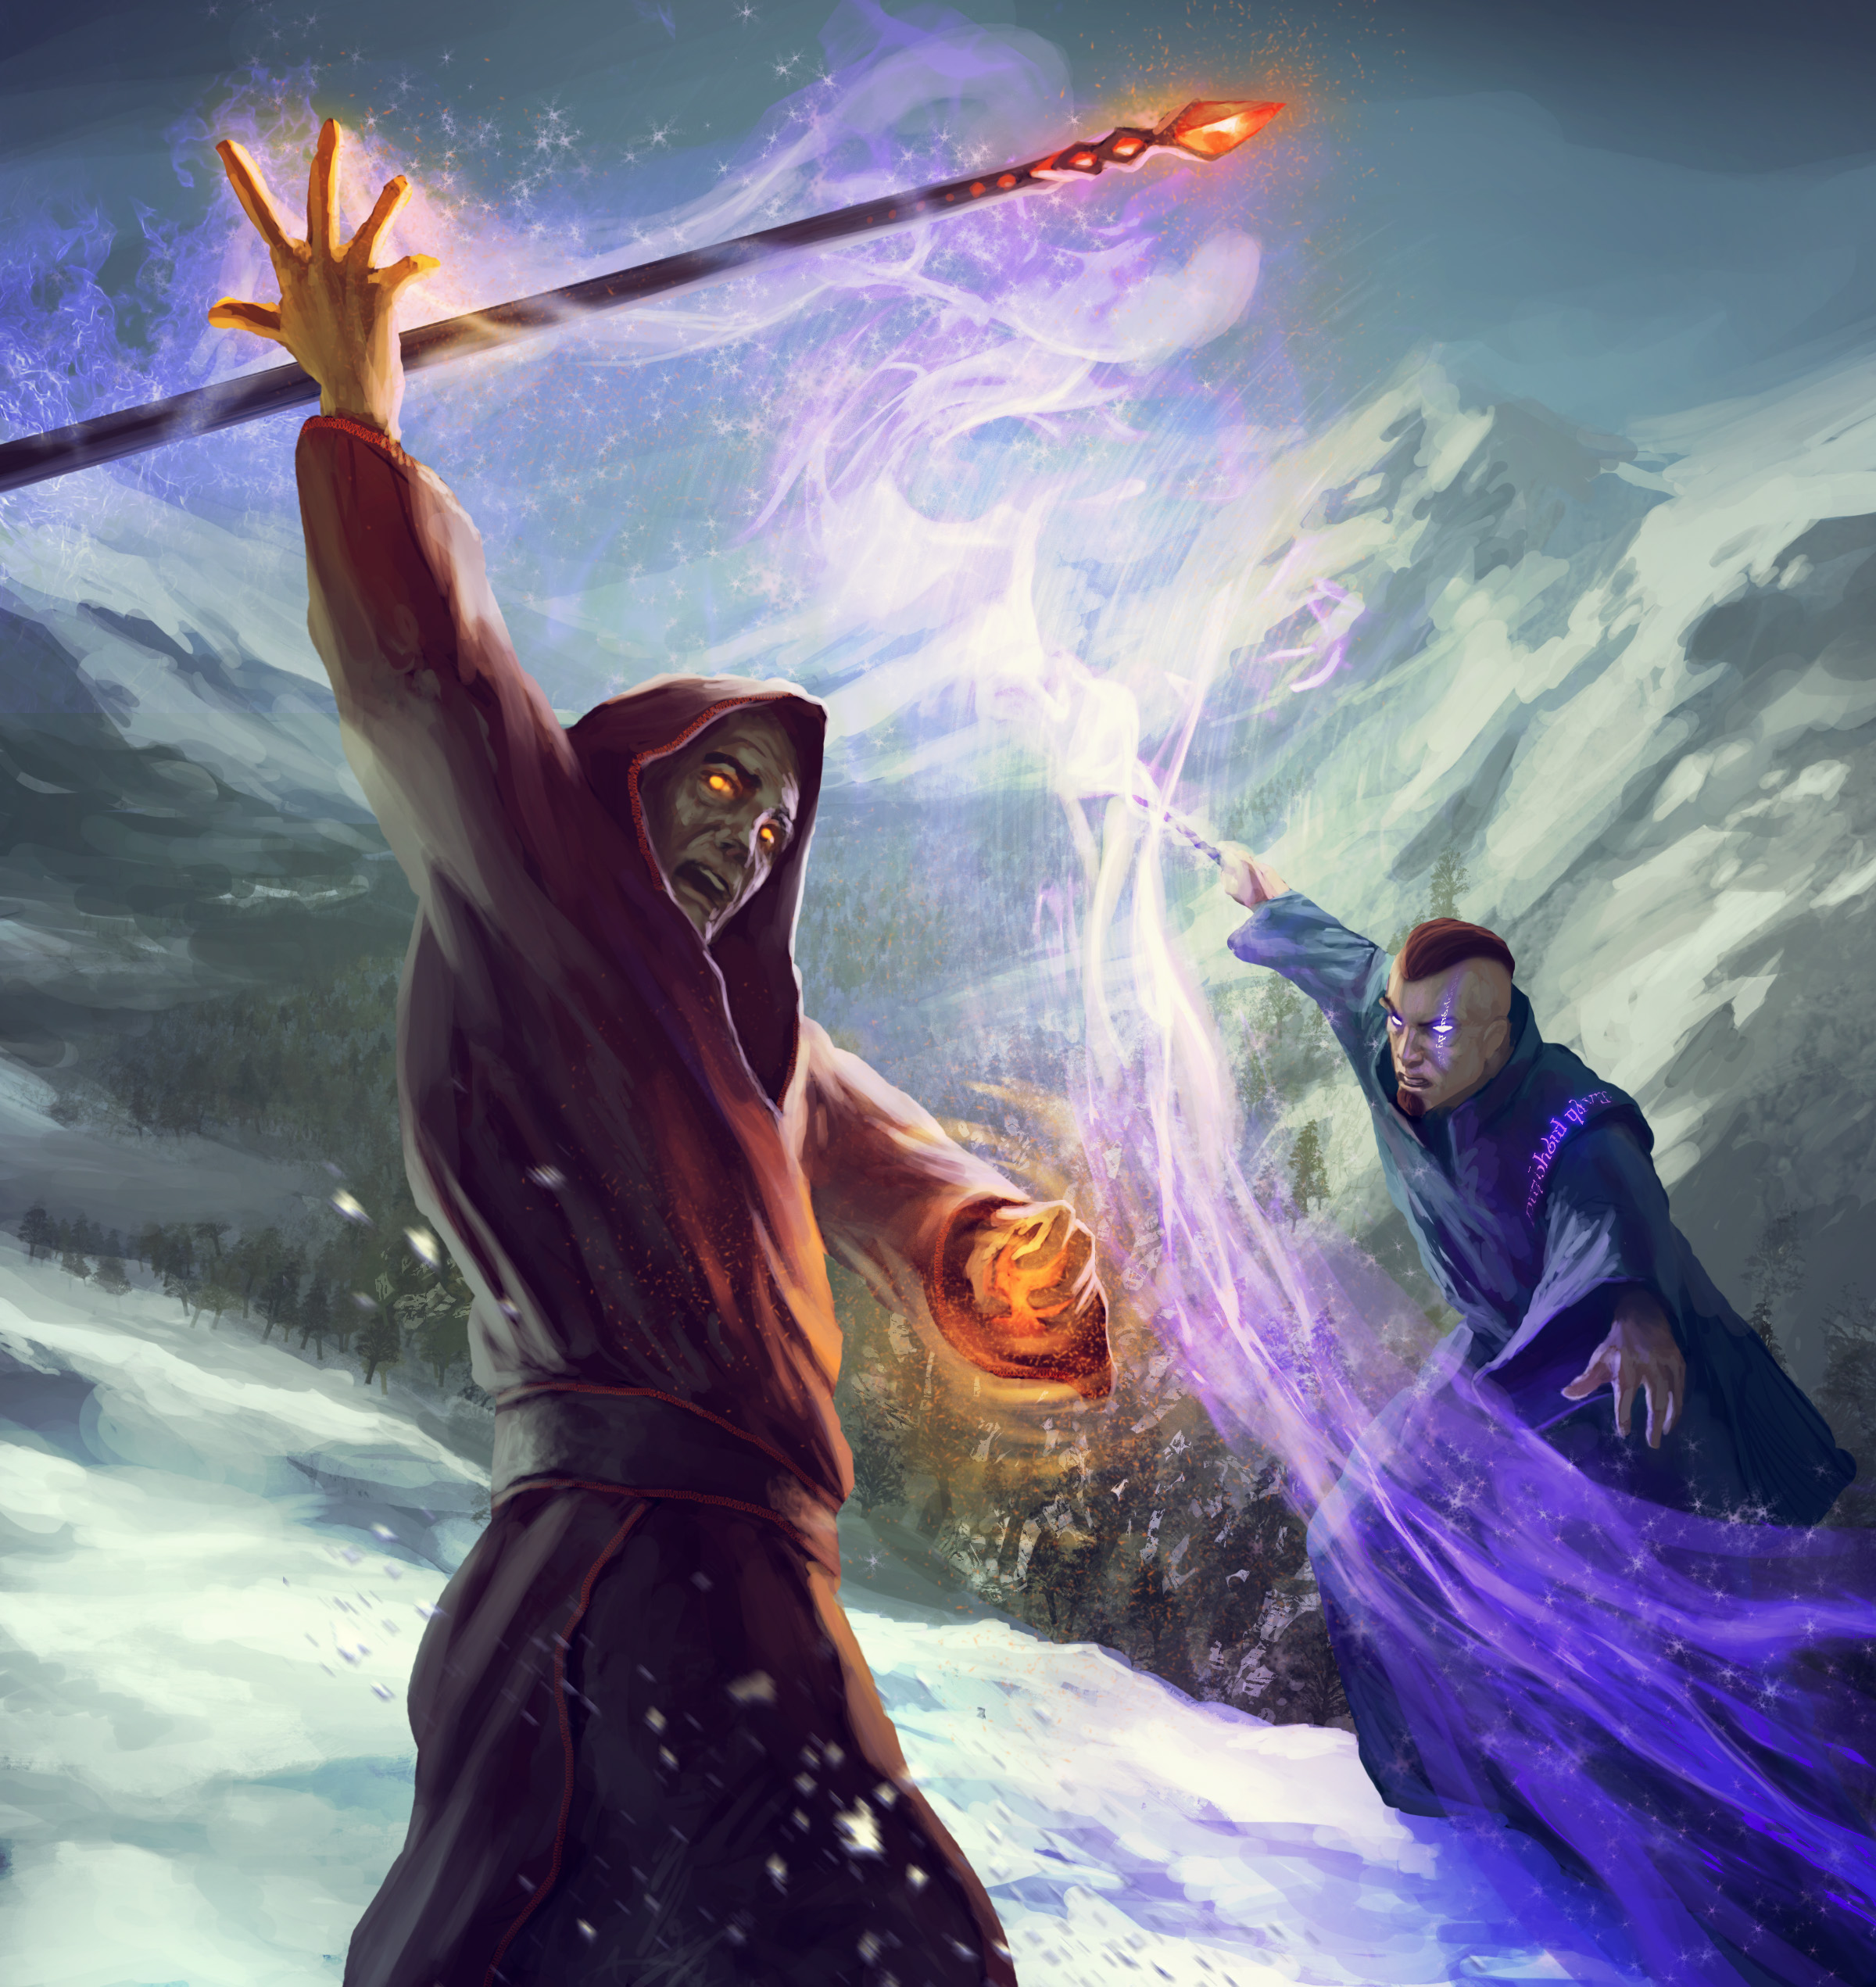
\includegraphics[scale=0.41]{img/sever_the_source_card_by_sirend.jpg}
\end{center}
\end{figure}


%\begin{samepage}
\begin{rpg-spell}
{Create Familiar}
{Permanent}

This spell allows the caster to make a personal sacrifice in order to create a Familiar. The Nature of the Familiar is dependent on the setting, but the spell typically only works on a non-sentient creature or inanimate object. The spell takes one hour to perform. The typical cost of ingredients for the spell is 100 Gold Pieces and it requires 3 Improvement Points. 

\begin{rpg-list}
\item An Arcane Magic user can have up to ½ their POW in Familiars, but few have more than one or two.
\item When a Familiar is destroyed or killed the Arcane Magic user loses 1D6 Hit Points from the trauma.
\item A Familiar gains sentience when created equal to 2D6 INT and Magic equal to 2D6 POW, unless the animal had a higher score, in which case that POW is used. 
\item A Familiar has a permanent mental connection with its master; with a range equal to 1/2 the caster’s POW in kilometres. Through this link the Familiar can allow the caster to ‘see’ through its perceptual abilities. The Arcane Magic user can cast spells on the Familiar as if touching it and the Familiar can cast any spells it knows on its master.
\item A Familiar can perceive its surroundings. How this happens depends on the type of Familiar. Animals can sense the world through their ordinary perceptions. Magical objects can detect the world around them up to a range equal to their POW in metres.
\item A Familiar dies when its master dies, and its life span is normal for the object or animal in which it is bound. It has Hit Points equal to the object or animal from which it was created.
\item Familiars may learn skills, but only ones they are capable of performing. Most Familiars in objects can only learn knowledge and magical skills. Animals have the skills that come naturally to them.
\item An animal Familiar can only be up to 1/2 the SIZ of the caster. 
\end{rpg-list}

\end{rpg-spell}
%\end{samepage}


%\begin{samepage}
\begin{rpg-spell}
{Create Scroll}
{Permanent}

These are written items which store Arcane Magic Spells.

All scrolls have an attached cost of 2 Gold Pieces per magnitude of spell in ingredients for special inks/parchments, etc.

The resulting scroll is a one use item, which upon a successful Arcane Magic Casting test, casts the spell(s) with any manipulations, at the magnitude that was cast on the scroll.

Alternatively, upon a successful Arcane Magic Casting the reader of the scroll can learn the spell by spending the appropriate number of Improvement Points.

Either way, upon a successful use of the scroll, the spell fades from the scroll. If the casting roll merely fails the spell remains, but the reader can not attempt to use the scroll until their Arcane Magic Casting skill increases. If the casting roll is fumbled the spell fades from the scroll, without any benefit to the reader.
\end{rpg-spell}
%\end{samepage}


%\begin{samepage}
\begin{rpg-spell}
{Create Spell Matrix}
{Permanent}

This spell creates items that store Arcane Magic spells. 
The enchanter pays 1 Improvement Point per spell stored in the matrix.

All spell matrices have an attached cost of 20 Gold Pieces per spell in special materials.

The wielder can cast and manipulate the spell at the skill of the original enchanter, using their own Power Points as fuel.

Spell matrices are mundane items in their own right and if the item is broken, then the spell is dispelled. However at the time of enchantment the enchanter can spend another Improvement Point to magically harden the item doubling its Hit Points and Armor Points.
\end{rpg-spell}
%\end{samepage}

%\begin{samepage}
\begin{rpg-spell}
{Damage Boosting}
{Touch}

This spell can be cast upon any weapon up to five ENC. Each point of Magnitude adds one point to the weapon’s damage (the basic spell will increase a hatchet from 1D6 damage to 1D6+1 damage, for instance). 
\end{rpg-spell}
%\end{samepage}


%\begin{samepage}
\begin{rpg-spell}
{Damage Resistance}
{Touch}

This spell protects the body of the recipient. Any incoming attack dealing damage equal to or less than the Magnitude of the spell is ignored. Any incoming attack dealing more damage than the Magnitude of Damage Resistance is unaffected and will deal its full damage as normal. Note that the protected character may still suffer from Knockback if applicable. 
\end{rpg-spell}
%\end{samepage}


%\begin{samepage}
\begin{rpg-spell}
{Diminish (Characteristic)}
{Resist(Persistence/Resilience), Touch}

There are actually seven Diminish spells, one for each Characteristic. The spell will temporarily apply a penalty to the specified Characteristic equal to the Magnitude of the spell. The penalty applied by this spell may not reduce a Characteristic below one and a creature must have the Characteristic in question to be affected by this spell. 

Diminish (STR, DEX, CON and SIZ) are resisted with Resilience. Diminish (INT, POW and CHA) are resisted with Persistence. 

Applying a penalty to POW does not reduce the character’s Power Points.

Note that not all uses of this spell are malicious. Thieves and others often value the timely use of a Diminish (SIZ) spell, as it can greatly enhance their ability to enter restricted areas. 
\end{rpg-spell}
%\end{samepage}


%\begin{samepage}
\begin{rpg-spell}
{Dominate (Species)}
{Resist(Persistence)}

This spell allows the caster to gain control over a creature belonging to a specific species. If the target fails to resist the spell, it must obey the commands of the caster for the duration of the spell. 

The controlled creature shares a telepathic link with the caster by which it can receive its orders. If the caster and the creature dominated do not share a common language, the caster can order it about by forming a mental image of the actions he wishes the dominated creature to perform.
\end{rpg-spell}
%\end{samepage}


%\begin{samepage}
\begin{rpg-spell}
{Energy Projection (Type)}
{Ranged, Instant, Resist(Dodge)}

Energy is either projected as a beam or a ball towards the target, which can avoid the attack by Dodging.

If the spell takes effect the target takes damage equal to double the Magnitude of the spell. Physical Armour does not protect against the damage, but magical protection does. Types of energy that can be projected by this spell are Cold (Dark), Lightning, Heat (Fire), Shards of Rock (Earth), Windblast (Air).
\end{rpg-spell}
%\end{samepage}


%\begin{samepage}
\begin{rpg-spell}
{Enhance (Characteristic)}
{Touch}

There are actually seven Enhance spells, one for each Characteristic. Essentially the reverse of the Diminish spell, Enhance allows the caster to temporarily apply a bonus to the specified Characteristic equal to the Magnitude of the spell. A creature must have the Characteristic in question to be affected by this spell. 

Applying a bonus to POW does not increase the character’s Power Points. 
\end{rpg-spell}
%\end{samepage}


%\begin{samepage}
\begin{rpg-spell}
{Fly}
{Concentration, Resist (Persistence)}

Using this spell allows the caster (or whomever or whatever he targets with the spell) to fly.  The caster may levitate a number of objects or characters (the caster counting as one of these characters if he so wishes). 

A levitated character may not be Overloaded and must have a SIZ Characteristic which is lower than the caster’s POW characteristic. 

Objects must have an ENC lower than the caster’s POW characteristic. 

Characters or objects moved by this spell have a base Movement Rate of 6m. All objects and characters moved by this spell move at the spellcaster’s behest, not their own. 

Each point of the spell’s Magnitude may either be used to increase the target’s Movement by +2m or to target an additional object or character – but not both. An Arcane Magic user casting this spell at Magnitude 4 may fly himself with a Movement of 12m, fly himself and a friend with a Movement of 8m each, or fly himself and three friends with a Movement of 6m each.
\end{rpg-spell}
%\end{samepage}


%\begin{samepage}
\begin{rpg-spell}
{Form/Set (Substance)}
{Instant}

There are an unlimited number of Form/Set spells in existence, one for every substance imaginable, from steel to smoke to water. 

Each point of Magnitude allows the caster to shape one ENC of solid substance or one cubic metre of an ethereal substance (like darkness). The caster must be Familiar with the shape he is forming. 

When the caster has finished the forming process, the substance retains its shape. Rigid substances like steel will hold the form they had at the end of the spell, while more mutable substances like water will immediately lose their shape. 

This spell can be used to mend damage done to an object. The caster must form the entire object and must succeed at an appropriate Craft test. If successful he will restore the item to its original condition. 

This spell can only be used on inanimate substances. 
\end{rpg-spell}
%\end{samepage}


%\begin{samepage}
\begin{rpg-spell}
{Glow}
{}

This spell causes a glowing point of light to appear on a solid substance. At its base, the spell creates an area of light one metre in radius, giving off the same illumination as a candle. Each additional point of Magnitude increases the radius of effect by one metre. At Magnitude 3, the brightness of the spell increases to that of a flaming brand at its centre. At Magnitude 5, it increases to that of a campfire and at Magnitude 10 to that of a bonfire. 

This spell can be cast on an opponent’s eyes. If cast on a living being the spell also gains the Resist (Dodge) trait. If the target fails to resist it, he will suffer a penalty to all attack, parry and Dodge tests, as well as any skills relying upon vision, equal to five times the spell’s Magnitude, until the spell ends or is dispelled. 
\end{rpg-spell}
%\end{samepage}


%\begin{samepage}
\begin{rpg-spell}
{Haste}
{}

Each point of Magnitude of Haste adds 1m to the Movement rate of the recipient. Every two points of Magnitude also adds +1 to the recipient’s Dexterity or Intelligence for the purposes of determining order in combat. 
\end{rpg-spell}
%\end{samepage}


%\begin{samepage}
\begin{rpg-spell}
{Hinder}
{Resist (Resilience)}

Each point of Magnitude of Hinder subtracts 1m from the Movement rate of the target. Every two points of Magnitude also subtracts 1 from the recipient’s Dexterity or Intelligence for the purposes of determining order in combat. 
\end{rpg-spell}
%\end{samepage}


%\begin{samepage}
\begin{rpg-spell}
{Holdfast}
{Touch}

This spell causes two adjacent ten centimetre by ten centimetre surfaces (roughly the size of a man’s palm) to commingle into one. The basic bond has a STR of 1. Each additional point of Magnitude will either increase the STR of the bond by +1 or double the area affected. 

This spell can affect organic and inorganic substances. If the caster is attempting to bond a living being with this spell, the spell gains the Resist (Resilience) trait.
\end{rpg-spell}
%\end{samepage}


%\begin{samepage}
\begin{rpg-spell}
{Mirage}
{Touch}

This is the Arcane Magic user’s version of Illusion. This spell creates an illusion based on all five senses. The illusion will seem real and solid unless the person looking at it succeeds in a Perception test. If the viewer succeeds in a Perception test and the Illusion could usually cause damage if believed in, it can no longer cause damage to that character. As soon as a viewer disbelieves the illusion it becomes insubstantial and ghost-like to him.

The Size and the strength of the illusion is governed by the Magnitude. A Magnitude 1 Illusion creates objects or creatures up to SIZ 10 and viewers have +60\% bonus to their Perception modifier test to disbelieve the illusion. For every extra Magnitude the caster can choose to either increase the size by 10 or apply a -20\% penalty to the Perception modifier test. Thus, with 5 Magnitude a caster could create a creature up to SIZ 30 with a Perception modifier of +20\%.
	
A positive Perception modifier means that the illusion is slightly fuzzy and unreal round the edges while a negative modifier means that it is indistinguishable from the real thing.
\end{rpg-spell}
%\end{samepage}


%\begin{samepage}
\begin{rpg-spell}
{Mystic Vistion}
{Concentration}

This spell allows the recipient to literally see magic. By augmenting the recipient’s natural vision, the spell allows him to see a creature’s Power Points, as well as enchanted items with their own Power Points or spells. The recipient must be able to actually see the creature or object for this spell to work. Mystic Vision also allows a recipient to see into the Spirit World.

On a normal success the recipient of the spell will only know roughly how many Power Points an object or creature has (1–10, 11–20, 21–30 and so forth). On a critical they will know exactly. On a fumble the Gamemaster should give the player a misleading total.

By looking at a spell effect, a recipient of Mystic Vision will automatically be aware of its magical origin (Arcane Magic, Divine Magic or Magic). By increasing the Magnitude of Mystic Vision, the caster can learn more about what he is seeing. Compare the Magnitude of Mystic Vision to the Magnitude of any spell that the target is either casting or under the influence of. As long as Mystic Vision’s Magnitude exceeds the other spell’s, the caster will be able to precisely determine the effects of the perceived spell, and a mental image of who cast the spell (if it is not obvious). 

By looking at an enchanted item, a recipient of Mystic Vision will automatically be aware of its gross magical effects (such as the types of enchantment currently on the item). Each point of Magnitude of Mystic Vision will also determine either the invested POW (and therefore the relevant strength) of a particular enchantment or a particular condition laid upon an enchantment, at the Gamemaster’s choice.
\end{rpg-spell}
%\end{samepage}


%\begin{samepage}
\begin{rpg-spell}
{Neutralise Magic}
{Instant}

This spell allows a caster to neutralise other spells. Neutralise Magic will eliminate a combined Magnitude of spells equal to its own Magnitude, starting with the most powerful affecting the target. If it fails to eliminate the most powerful spell then it will instead target the second-most powerful spell. As soon as Neutralise Magic can no longer dismiss a target’s spells, because all the remaining spell’s Magnitudes are too high, its effects immediately end. 

Neutralise Magic can be fired as a Reaction, but only when another spell is cast within Neutralise Magic’s Range that the character wishes to counter. A successful Neutralise Magic disrupts the other spell and nullifies it. As long as Neutralise Magic’s Magnitude equals or exceeds the target spell’s Magnitude, the target spell is countered. 
\end{rpg-spell}
%\end{samepage}


%\begin{samepage}
\begin{rpg-spell}
{Other World Portal (Other World)}
{Instant}

This spell creates a portal to a named Other World. The Magnitude of the spell is the number of creatures (SIZ 12-18) who can use the portal simultaneously. The portal exists as long as the spell is in effect. When the spell’s duration is reached, the portal closes instantly. 

If the spell casting is fumbled, catastrophic events occur. Here are some example events but the creative Gamemaster is encouraged to create more:
\begin{rpg-list}
\item A malignant creature from that Other World goes through the portal and attacks the caster, in an attempt to close the portal. 
\item The caster and all within 10m of him are sucked through the portal, which then promptly closes. Worse the caster is so befuddled that he cannot remember this spell for D20+D4 hours.
\item The Other World, to which the portal is connected, invades the home reality in a 1D10 km diametre from the portal. The home reality protects itself by throwing up a magical barrier that lets things into the beachhead but not out. 
\end{rpg-list}
\end{rpg-spell}
%\end{samepage}


%\begin{samepage}
\begin{rpg-spell}
{Palsy}
{Resist (Resilience)}

If the caster is able to overcome his target with this spell, he can turn the victim’s own nervous system against him. The spell will paralyse the target, provided the spell’s Magnitude is greater than the quarter of target’s current Hit Points. 
\end{rpg-spell}
%\end{samepage}


%\begin{samepage}
\begin{rpg-spell}
{Protective Sphere}
{}

When completed, the Protective Sphere will create a sphere-shaped area of protection with a radius in metres equal to the spell’s Magnitude. If this spell is cast on the ground (or other immovable place) it cannot be moved. If cast on a vehicle (such as the bed of a wagon) or a person, it will move with the target.  After the sphere has been completed any one or all of the following spells can be added to provide the defensive capacities of the Sphere during the duration of the Sphere: Damage Resistance, Spell Resistance, Spirit Resistance. The Sphere on its own provides no protection.

The Protective Sphere’s perimetre contains the benefits of its combined Resistance spell(s). The Protective Sphere only inhibits spells or attacks entering the circle from the outside – attacks or spells originating within the circle are unaffected. Thus a Protective Sphere against spirits would block out outside spirits but have no effect on those already inside its perimetre. A Protective Sphere against damage or spells would block out incoming attacks/spells, but have no effect on those attacks made within the sphere (including attacks targeting those outside the sphere). 
\end{rpg-spell}
%\end{samepage}


%\begin{samepage}
\begin{rpg-spell}
{Regenerate}
{Concentration Special, Instant, Touch}

This spell causes a severed or maimed limb to regrow or reattach. Regenerate cannot return a character from the embrace of death. 

The Magnitude of the spell must equal or exceed the maximum Hit Points lost as a result of the Major Wound taken. This spell will cause a limb severed by a Major Wound to regrow or, if the detached limb is still present, for the limb to reattach itself to its stump. 

Regenerate takes a number of minutes equal to the target’s SIZ to reattach a limb, during which time the caster must maintain concentration on the spell. The Hit Points lost due to the Major Wound are recovered at the end of this period.
\end{rpg-spell}
%\end{samepage}


%\begin{samepage}
\begin{rpg-spell}
{(Sense) Projection}
{Concentration}

Each (Sense) Projection spell is a separate spell. Each spell encompasses one of the five base senses but there are also variants for any unusual sensory mechanism appropriate to the game world (such as sonar). 

This spell allows the caster to project one of his senses anywhere within the spell’s Range. The spell forms an invisible and intangible sensor, some ten centimetres across, which receives the specified type of sensory input and transmits it to the caster. The sensor can move a number of metres per Combat Round equal to the spell’s Magnitude at the caster’s direction and allows him to use his Perception skill through the sensor. 

Spells can be cast through the sensor of some Projection spells. For instance, ranged spells require Sight Projection, while touch spells require Touch Projection (and likely Sight Projection too, simply so the caster can find his target efficiently). 

Characters using Mystic Vision can see the sensor and attack it if they wish, though it is only vulnerable to magic. Magical weapons and spells employed against the sensor will not destroy it but will instead transfer their damage directly to the caster.
\end{rpg-spell}
%\end{samepage}


%\begin{samepage}
\begin{rpg-spell}
{Sense (Substance)}
{Concentration}

Eminently useful for finding valuables from afar, this spell has a variation for every substance imaginable. Sense (Substance) will cause all sources of the substance within range of the spell to glow an appropriate colour visible only to the caster – diamonds will gleam like ice, amber will shine like a camp fire and so on. Each point of this spell’s Magnitude allows it to penetrate one metre of rock, wood or dirt. If the source is concealed behind such a material, the surface nearest the caster will glow for a moment. The spell cannot penetrate refined metal, though it can penetrate ore. 
\end{rpg-spell}
%\end{samepage}


%\begin{samepage}
\begin{rpg-spell}
{Shapechange (Species) to (Species)}
{Resist (Resilience), Touch}

Each Shapechange spell is a separate spell. Of all spells with multiple variations, the Shapechange spell has the most, comprising a new spell for almost every combination of creatures imaginable. The spell only works on living things – the dead or inanimate cannot be shapechanged. 

The Magnitude of the spell must be equal to or greater than the average SIZ of both specified species. Thus changing a mouse (SIZ 1) into a newt (also SIZ 1) is Magnitude 1. Changing a mouse into a lion (SIZ 19) is Magnitude 19. 

If the spell is successful, the target will be biologically changed, gaining the STR, DEX, CON and SIZ of its new form. Its INT, POW and CHA are unchanged, and the target retains its memories and abilities (though it may be unable to use some of those abilities in its new form). 
\end{rpg-spell}
%\end{samepage}


%\begin{samepage}
\begin{rpg-spell}
{Skin of Life}
{Touch}

This spell protects the recipient from suffocation by air deprivation, due to such factors as drowning or the Smother spell. Each point of Magnitude will cover three points of SIZ – thus a Magnitude 4 Skin of Life spell would sustain a SIZ 12 creature. 
\end{rpg-spell}
%\end{samepage}


%\begin{samepage}
\begin{rpg-spell}
{Smother}
{Concentration, Resist (Resilience Special)}

If successful, this spell neutralises the air surrounding the target, making each breath stale and worthless, depriving it of oxygen. The caster must concentrate each round, in order to keep the spell operating. For the duration of the spell, the target will be unable to breathe, essentially drowning on dry land. 

When the spell begins, the target’s Resilience test determines whether it is able to gasp in one last breath before Smother cuts off the surrounding oxygen supply. If the target succeeds, it may hold its breath as normal. If it fails, it will start drowning in the next Combat Round. 

This spell can also be used to extinguish fires, as the flames will be starved of oxygen. At Magnitude 1, it can extinguish a Flame, Magnitude 2 a Large Flame, Magnitude 4 a Small Fire, Magnitude 7 a Large Fire and Magnitude 10 it will put out an Inferno. Smother has no effect on magical fire or on fire-based creatures. 
\end{rpg-spell}
%\end{samepage}


%\begin{samepage}
\begin{rpg-spell}
{Spell Resistance}
{}

This spell matches its Magnitude against the Magnitude of any incoming spell. If Spell Resistance’s Magnitude is greater than the incoming spell’s, then the incoming spell has no effect. If the incoming spell’s Magnitude is equal to or greater than the Magnitude of Spell Resistance, then the spell affects the target normally. 

Unlike many protective spells, Spell Resistance remains in place for the entirety of its Duration – spells that successfully breach the spell do not dispel it. However, it does not discriminate between incoming spells – a comrade attempting to magically heal the recipient of Spell Resistance must overcome it in order to successfully use a healing spell. 
\end{rpg-spell}
%\end{samepage}


%\begin{samepage}
\begin{rpg-spell}
{Spiritual Projection}
{Touch}

Spiritual Projection causes the recipient’s soul to leave its corporeal body and manifest in the Spirit World. The recipient’s corporeal body slumps into a catatonic state for the remainder of the spell.  While Spiritual Projection is sometimes used for scouting purposes (as the recipient’s spirit can pass through nearly any obstacle) it is usually used to combat or confront Spirit World denizens.

The recipient’s body remains vulnerable for the Duration of the Spiritual Projection. The soul will always know the direction its host body lies in, and the rough range to it in metres, but it cannot use the body’s senses. It is quite possible for a wandering soul to have its body destroyed and not realise it until it returns from its sojourn. It is also possible for a wandering spirit to possess the host body, leaving the wandering soul trapped as a spirit, at least until the spell ends and the soul dies. It is for these reasons that most Arcane Magic users ensure that their bodies are in a safe stronghold and protected by Damage, Spell and Spirit Resistance, before casting Spiritual Projection.

As a traveller in the Spirit World, the recipient automatically gains the effects of Mystic Vision for the duration of his Spiritual Journey. However, he will suffer a –40\% penalty to all Perception tests to spot mundane items or events in the real world while in the Spirit World. A recipient may not travel further from its host body than the Range of the spell and it can move at double their normal rate.

	While on the Spiritual Journey the recipient otherwise obeys all the other rules that a Shaman does (see chapter \ref{ch:shamanism}) as regards skill use as well as initiating Spirit Combat. They may opt to use their Arcane Magic skill to make attacks, if it is higher than their Persistence. For the duration of the Spirit Combat the Spirit Damage of the Character is increased from 1D4 to 1D6.
\end{rpg-spell}
%\end{samepage}


%\begin{samepage}
\begin{rpg-spell}
{Spirit Resistance}
{}

This spell matches its Magnitude against the POW of any spirit that comes into contact with the recipient. If the recipient of the spell’s combined POW + Spirit Resistance’s Magnitude is greater than the spirit’s POW, the spirit cannot touch the recipient. 

A spirit unable to touch a recipient will not be able to personally attack or harm him, including through ranged attacks. A spell cast by a spirit at the recipient is blocked unless its Magnitude exceeds the Spirit Resistances’s Magnitude. 
\end{rpg-spell}
%\end{samepage}


%\begin{samepage}
\begin{rpg-spell}
{Summon (Other World Creature)}
{Resist (Persistence)}

This spell allows the caster to summon one Other World creature, per casting, to the mundane world. The creature is not automatically under the caster’s control. If the summoned creature succeeds its Persistence test, it is free of the caster's command and if so inclined may be hostile to the caster. Otherwise it acts as if under the influence of a Dominate spell, for the Duration of the spell. The Duration of the summon spell also determines how long the creature is trapped in the mundane world.

Examples of of spell variations: Demons, Elementals, Spirits and Undead.
\end{rpg-spell}
%\end{samepage}


%\begin{samepage}
\begin{rpg-spell}
{Tap (Characteristic}
{Concentration, Resist (Persistence), Touch}

There are actually seven Tap spells, one for each Characteristic. These devastating spells allow the caster to permanently strip a target of Characteristic points, transforming them into Power Points for his own use. 

The caster must make contact with the target, either physically or through Touch Projection, in order to Tap it – therefore the spell cannot be used on incorporeal creatures, such as spirits. 

Tap will only work if its Magnitude is equal to, or greater than the target’s specified Characteristic. Thus a Magnitude 6 Tap Strength spell would only work on targets with a STR of 6 or lower. 

The number of points Tapped by the spell are equal to 1D6 per Combat Round the Spell is applied to the Victim.

Characteristic points lost to Tap are lost permanently, though the victim can raise them again through normal means of increasing a Characteristic. Characteristics may be Tapped to 0, which usually involves the death of the victim. The exception being Charisma.

For each Characteristic point the caster Taps, he will gain one Power Point. The caster is limited in the number of Power Points he can gain through Tap; the spell can only increase his Power Points to double his normal limit. An Arcane Magic user may simply Tap a target and dissipate any gained Power Points. 

If the caster gains more Power Points through Tap than his normal maximum, they will disappear at the rate of one Power Point per minute once the spell finishes. 
\end{rpg-spell}
%\end{samepage}


%\begin{samepage}
\begin{rpg-spell}
{Teleport}
{Instant, Resist (Dodge)}

Teleport allows an Arcane Magic user to instantaneously move himself, or a target, to anywhere within the range of the spell, as long as the destination can be directly observed (Sense Projection spells allow the Caster to ‘see’ locations beyond physical line of sight), there is solid footing and no object bars their arrival. If these conditions are not met, the spell automatically fails. The caster is able to teleport objects up to 3 points of SIZ per point of Magnitude.
\end{rpg-spell}
%\end{samepage}


%\begin{samepage}
\begin{rpg-spell}
{Time Travel (Time Period)}
{Instant}

This spell transports the caster and a number of creatures (of SIZ 12-18) equal to the Magnitude of the spell to a named Time era via a Time Tunnel that opens up and instantly sucks them through to their destination. The Duration of the spell is the time that the caster and group jumps forward or backwards through time. 

Casters usually have some knowledge about the time period they are travelling to, and use an Anchor, a landmark such as a bronze statue, that exists in both the original and destination time period. If they are travelling blind without such an Anchor, the casting roll is at -20\% and the effects of a fumbled roll are even more catastrophic than the examples below suggest. 

If the spell casting is failed, the caster and group still travels, but they end up in the wrong location (1D10 Km away from the Anchor point) and time (1D10 time units away, the length of the time unit depends on Duration, e.g. if the duration was in days, the time unit is days).

If the spell casting is fumbled catastrophic events occur. Here are some example events; the creative Gamemaster is encouraged to create more:
\begin{rpg-list}
\item A Guardian creature from an Other World emerges from the portal and attacks the caster, in an attempt to close the portal. 
\item The caster, and all within 10m of him, is sucked through the portal which then promptly closes. The caster is so befuddled that he cannot remember the spell for D20+D4 hours. 
\item As above, but the caster and party arrive in a completely different Time Era or even an Alternative Reality.
\end{rpg-list}

Arcane Magic users with this spell can change time freely without having to worry about unintentional butterfly effect changes, or any alterations in their own existence or memory from changing their past. However, too regular use is likely to lead to the catastrophic effects of a fumble.
\end{rpg-spell}
%\end{samepage}


%\begin{samepage}
\begin{rpg-spell}
{Treat Wounds}
{Instant, Touch}

This spell must be cast upon a wounded character. It dramatically accelerates the natural healing rate of the target.  For every point of Magnitude of this spell, the caster can repair one hit point per Combat Round, for the Duration of the spell. Treat Wounds cannot reattach or regrow a severed limb and will not work on any Major Wound effects. 
\end{rpg-spell}
%\end{samepage}


%\begin{samepage}
\begin{rpg-spell}
{Venom}
{Resist (Resilience), Touch}

This spell infuses the target’s body with a magical poison. The Potency of the poison is equal to the spell’s Magnitude x 5, takes effect instantly, and does damage equal to the magnitude per combat round for the spell’s Duration. The target may resist the poison with a Resilience test, as normal.
\end{rpg-spell}
%\end{samepage}


\section{Creating Magic Items}
Most Magic Items found in play in a game of Fantasy D100 will have been created by the characters or Non Player Character magicians.

Although the spells that their characters use to create Magic Items are detailed in their respective spell lists, its worth going through them briefly to remind yourself what spell does what and how it is used.

\begin{description}
\item [Create Scrolls] This spell allows for the creation of magical writings. Scrolls can be used to transfer knowledge (spells) or directly to cast the written spell.
\item [Create Spell Matrix] Arcane Magic users can create items and store spells using this spell. Spells stored can then be used and manipulated using the wielder's Power Points.
\end{description}

Arcane Magic users also find very useful the Magic spell Create Power Point Store so that they can have a greater pool for manipulations.

\subsection{Identify a Magic Item}
There is no catch all “Detect Magical Properties” or “Know Magic item” skill in Fantsy D100. This is quite deliberate, keeping with the general policy that such items are not the equivalent of Magical shotguns.  Some options are:

Consult a Sage or other magical expert. This option will cost the characters lots of money. Take a baseline of one hundred silvers per point of spell magnitude OR some perilous quest that the character must do in return. Such experts are rare, because most high ranking Magicians have little time for magical research for others, and would be more interested in their own schemes. 

Detect Magic spells. This merely tells you the item is magical.  A critical casting may tell the caster how powerful the item is.

Trial and error. The character tries to find out the item’s use by experiment. Allow creative and imaginative plans to reveal partially what the item does.

Researching the myths and legends around the item.  This is the most certain way of finding out what a magic item does. Of course such myths may be obscure themselves, requiring a dangerous adventure to a long hidden repository of knowledge to find.


\chapter{Divine Magic}
\label{ch:divine}

This type of magic is gained through the worship of a god or goddess. Divine Magic spells come directly from the Deity and given to the character to use on their Deity’s behalf. 

The first step in learning Divine Magic is to join a religion that worships the Deity whose magic the character wants to learn.

\section{Religions}
Religions range in size from a handful of worshippers, meeting in secret to honour a dead hero of the revolution, to the millions of devotees of a world spanning sun god. There are temples where worshippers can learn Divine Magic directly from their Deity. They have rules and expectations of their worshippers and anyone found wanting is expelled from the comfort and support of the religion. 

\subsection{Religion Template}
Each religion is described using the following Religion format.
\begin{description}
\item[Name of God or Religion]
\item[Short description:] This short description briefly covers the religion’s mythology and its current place in the world.
\item[Type of Religion:] This is the type and size of religion. Great Deities are worshipped by millions and are at least acknowledged across the entire world. Major Deities are important in a specific region and have hundreds of thousands of worshipers. Minor Deities are usually the minor members of a religious pantheon appealing to a small group of specialist worshipers. Hero Religions worship dead heroes whose deeds and magic powers live on after their death.
\item[Worshippers:] The type of people who typically make up the religion membership.
\item[Worshipper Duties:] This is what the god and religion expect of its members. Break these rules and expect expulsion. On the other hand, follow these rules and promote them to others and the character will advance in the religion’s hierarchy.
\item[Religion skills:] These are skills favoured by the religion’s patron Deity and taught to its worshippers by its Priests.
\item[Religion spells:] Divine Magic that the god teaches.
\item[Special benefits:] Any bonuses to skill use or other special abilities or advantages that a worshipper gains by being a member of the religion.
\end{description}

Several examples can be seen in section~\ref{ssec:deities}.

\subsection{Worshipper Duties}
Each religion has a set of Worshipper Duties which represent the religion’s objectives in the world.

When a character does an action that fulfils one of the Worshipper Duties they gain one Improvement Point for a minor act and up to three points for a major act.

When a character does an action that goes against one of the Worshipper Duties they lose between one and three Improvement Points, depending on the grievousness of their transgression. If they have no Improvement Points left, then they start to lose Divine Magic spells learnt from the religion as a penance, on a one to one basis. The player may choose which spell to lose, but they must be ones that they have learnt from the religion.

\begin{rpg-examplebox}
Gerik the Pious acts in away that brings his god into disrepute and loses an Improvement Point. He has no Improvement Points to lose, since he has previously spent them on religion improvements, so he loses Shield 3 which he had previously learnt from the religion, which now becomes Shield 2.
\end{rpg-examplebox}

If the offending character has no Improvement Points or spells to lose, then they are excommunicated from the religion and may never join it again.

\subsection{Religion Ranks}
There are four ranks of membership: lay members, Initiates, Priests and Holy Warriors.

\subsubsection{Lay members}
Lay members are normal worshippers of the religion. They regularly attend the temple on holy days and do their best to uphold the strictures of the religion. In return, the religion protects them as best it can, and its Priests and Initiates cast Divine Magic on their behalf. Lay members cannot learn Divine Magic. To become a lay member of a religion a character must have Lore (Religion) of at least 20\%. 

\subsubsection{Initiates}
Initiates are worshippers who have dedicated their lives to the tenents of the religion. They always attend the temple on holy days and always uphold the strictures of the religion. In return, the religion will pay ransoms if they are captured and teach the Initiate Divine Magic. Initiates can learn up to 2 Magnitude of any Divine Magic spell available to the religion. To become an Initiate a member of a religion have a Lore (Religion) of at least 40\% and pay an Improvement Point cost of two points.

\subsubsection{Priests}
Priests are the living embodiment of their faith, instructed by their Deity to be its living representative in the mortal world. They lead the services for their temple on holy days. In return, the religion will pay ransoms if they are captured and teach them the inner secrets of their religion (this means all available Divine Magic at unlimited Magnitude). To become a Priest a character must have a Lore (Religion) and two of the cult skills at least 75\%, there must be a vacancy in the temple hierarchy, or the Priest be willing to become a missionary and establish a new temple. In addition the Player must pay five Improvement Points.

Upon becoming a Priest the character gains an Allied Spirit. This is a spirit associated with the Deity who is willing to work with one of their mortal worshipers to further the aims of the religion. The Allied Spirit is usually bound in either an animal or an item, sacred to the religion. If this item or animal is destroyed then the Allied Spirit returns to its home plane of existence. A Priest must go on a Quest of Repentance, which directly benefits his religion to gain a new Allied Spirit, since the Gods look dimly on Priests who lose their Allied Spirits.

An Allied Spirit starts with an INT of 2D6+6 and a POW of 3D6 and knows 3 points of Divine Magic known to the Religion. The spirit can see immaterial and invisible spirits, alerting its master to their presence in a twenty meter range. An Allied Spirit is in permanent Mind Link with its master, with a range equal to its POW x5 in meters. 

An Allied Spirit has whatever physical characteristics that its host animal or item has. Allied Spirits can be improved like player characters, by spending Improvement Points from their master’s total.


\subsubsection{Holy Warriors}
These are Holy Warriors who protect the temples and worshipers of their Deity. Not all Religions have Holy Warriors, especially those dedicated to peace, but where they do, these warriors ceaselessly crusade to protect the faithful and punish the Religion’s enemies. Like Priests they are expected to uphold the Worshipper duties unfailingly. Also, as the religion’s warriors, they are expected to take up arms against any aggressor who attacks its worshippers or the religion’s Temples.

These warriors are incredibly useful to the cult they belong to, which will always pay any ransom or make a rescue attempt when a Holy Warrior is captured. In addition they teach them any Divine Magic known to the religion.

The minimum requirement to become a Holy Warrior is to have Lore (Religion) of at least 50\% and a Weapon Skill of 75\% in the Religion’s holy weapon, usually the weapon that is most associated with the Deity that the Religion worships. In addition the Player must pay five Improvement Points.

When someone becomes a Holy Warrior they are gifted a specially consecrated weapon, that gives them a bonus when fighting to defend fellow worshippers, religion temples, and when attacking enemies of their faith. This bonus is usually +20\% to the appropriate weapon skill and double damage when fighting for their Religion. All damage done by such weapons is considered magical.

They also gain armour, which is magically blessed by the Religion’s Deity. Normally, this is at least double the normal AP of the armour type used, and it may have additional powers depending on the Deity.


\subsection{Player Character Priests}
Priests and Holy Warriors don’t just hang around their Temples doing their duties. They have plenty of Initiates and lay worshippers to do the more mundane administrative tasks, such as collecting tithes and feeding the poor. As player characters, their lives are more interesting and the source of constant Questing on behalf of their religion. Some of the Quests that they might get involved in are as follows:
\begin{rpg-list}
\item Going out and converting the unbelievers (or those who believe in the wrong Deity).
\item Actively fighting the enemies of the religion.
\item Recovering long-lost symbols and powerful artefacts of the faith. 
\item Attending a cross-faith to deal with all the politics and misunderstanding to come to a consensus about what to do about a common enemy.
\item Rushing to the aid of an embattled and besieged town of his faithful believers beset by enemies or some other form of spiritual peril.
\item Visiting the hinterlands to provide spiritual guidance and duties to those in need
\item Traveling to a distant Holy Mountain to commune directly with their Deity or otherwise performing idealistic inspirational acts, or to prove their worth.
\item Going on special mission, where success depends on Divine Magic.
\item Traveling as a special envoy of the Religion to show due deference to the King / Priest / High Emperor.
\end{rpg-list}


\subsection{Deities}
\label{ssec:deities}
The following Religions are intended as templates for either your own creations as simple pick up and play religions, that can be elaborated and detailed as a campaign progresses.

\subsubsection{The Night Mistress}
\subsubsection{The Sun King}
\subsubsection{The Sky Lord}
\subsubsection{The Earth Mother}
\begin{description}
\item[Description:] The all embracing and loving Earth Mother is known throughout the world. Some people believe that she is the world itself. She is the source of all nature’s bounty, which clothes and feeds mankind, but also has a savage side that expresses itself in hurricanes, tidal waves and other natural disasters. 
\item[Type of Religion:] Great Deity
\item[Worshippers:] The religion is made up of people and creatures who live off the land. In civilised areas these are the peasants who farm the land and the woodsmen who hunt and gather in the forests. In the wilderness the Elves, Satyrs and Fey worship her. She is found wherever creatures have an acknowledged connection with nature.
\item[Worshipper Duties:] Respect the Earth. Don’t foul or pollute the environment. Practice the peaceful cut, a small prayer said in thanks to the animal spirit before killing it for food. The prayer ensures its return to the Earth Mother and through the cycle of rebirth into the world. 
\item[Religion skills:] Healing, Nature Lore, Resilience.
%\item[Magic:] Heal, Protection
\item[Divine Magic:] All common spells, Absorption, Berserk, Heal Body.
\item[Special benefits:] Any member of this cult gains a +20\% bonus to their Nature Lore, due to their connection to Nature, which they gain through their relationship with the Earth Mother.
\end{description}


\subsubsection{The Death Goddess}
\subsubsection{The Lord of Knowledge}
\subsubsection{The Trickster}
\subsubsection{The Merchant}
\subsubsection{The Hearth Goddess}
\subsubsection{The Lord of War}
\subsubsection{The Healer Goddess}
\subsubsection{The Sea Goddess}
\subsubsection{Chaos}
\subsubsection{The Moon Hag}
\subsubsection{The Huntress}



\begin{rpg-examplebox}
Earth Mother Pristess represent the divine Earth Mother at the religion’s rituals and it is acknowledged that she speaks through them.

Earth Mothers usually bind their Allied Spirits into animals local to their temple, such as Cows in urban areas, or Foxes and Bears in mountain areas. If a suitable animal is not available branches taken from local trees are satisfactory. 

Due to the nature of the religion, most are female but very rarely a male with a strong feminine side will meet the requirements.
\end{rpg-examplebox}


\begin{description}
	\item[Apprentices:] Students of Sorcery who will only know a couple of spells, usually including Mystic Vision, at a base of 40\%. 
	\item[Adepts:] Graduates of the schools of wizardry or equivalent. They will know between five and ten spells, and will have a Sorcery Casting skill ranging from 50\% to 90\%.
	\item[Magus:] Acknowledged masters of Sorcery. They will have at least ten spells and a Sorcery Casting skill of 90\%+.
\end{description}

\section{Spot Rules}

\subsection{Learning Sorcery}
Sorcery is governed by the Sorcery Casting magical skill. The base chance for Sorcery Casting is INT. Spells are learnt separately, but the Sorcery Casting skill determines the success for casting all Sorcery spells. Characters learn Sorcery from other characters who know the practice. It costs ten Improvement Points to get access to the Sorcery discipline. 

\subsection{Learning Spells}
Before a spell can be cast using Sorcery, the following process must be followed:
The character must first learn the spell through research. In order to learn a particular Sorcery spell, the caster must possess the spell in written form or be taught it by a teacher. In game terms this means having access to a teacher who knows the spell or a book or scroll where it is written down. The player then spends two Improvement Points and writes the spell down on their character sheet. Once the Sorcery spell has been learned, the character will be ready to try casting it.



\subsection{Casting Spells}
A character must be able to gesture with his hands, and be able to chant, in order to cast a spell. Whenever a spell is cast using Sorcery, there will always be a sight and sound that nearby creatures can detect, be it a flash of light, a crack of thunder, or a shimmering in the air. The exact effects are up to the Games Master and Player to decide , but will automatically be detected by any creatures within ten times the Magnitude of the spell in metres. 

Casting a Sorcery spell requires a successful skill test using the Sorcery Casting skill. If successful, the spell takes effect. If the casting test fails, the spell does not take effect. 

\subsubsection{Power Points}
All Sorcery spells cost a base of one Magic Point to cast. Sorcery spells can be modifying as the caster wishes (if he has the appropriate power points). If a Manipulation effect is applied to a spell, each effect costs one Power Point to apply (see below). 

The result of the Sorcery casting test depends on its success:
\begin{description}
	\item[Success:] A number of Power Points are deducted from the spellcaster’s total, equal to the Manipulation effects Power Points plus one of the spell. The spell then takes effect.
	\item[Failure:] The spell does not take effect and the character loses the spell's Power Points.
	\item[Critical:] Any attempt to resist or counter the spell suffers -20\% penalty. Moreover, only the base cost of one Power Point is lost (not for any Manipulations).
	\item[Fumble:] The spell fails and the Sorcerer loses 1D6 Power Points in addition to normal Power Point loss.
\end{description}


\subsubsection{Casting Time}
No other Combat Action may be taken while casting a spell, though the character may slowly walk up to half their Movement. 

A spell takes effect at the end of its casting, which starts at the beginning of the Combat Round and ends on the INT of the Caster in the Combat order. Note that while spellcasting, a character will draw possible attacks from enemies they are adjacent to during a Combat Round. 

Distractions or attacks on the spellcaster as he casts will either automatically ruin the spell (if the spellcaster is blinded or disarmed, or suffers a Major Wound) or require Persistence tests for them to maintain concentration on the spell. 

\subsubsection{Spell Manipulations}
Sorcery spells have three basic effects which can be manipulated by the caster: Magnitude, Duration, and Range.

Each effect has a default value which the spell can be cast at, costing one Power Point. The default value for the spell effects are listed in table~\ref{tab:sorcery-manipulations}.

\begin{table}
\begin{center}
\caption{Sorcery Manipulations}
\label{tab:sorcery-manipulations}
\begin{rpg-table}[|c|c|c|Y|]
        \hline
	\textbf{Power Points}  & \textbf{Magniture} & \textbf{Duration} & \textbf{Range}\\
        \hline
	1 (Default) & 1 & 5 minutes & 10m\\
	+1 & 2 & 15 minutes & 20m\\
	+2 & 3 & 30 minutes & 40m\\
	+3 & 4 & 1 hour & 80m\\
	+4 & 5 & 2 hours & 160m\\
	+5 & 6 & 4 hours & 320m\\
	+6 & 7 & 12 hours & 640m\\
	+7 & 8 & 1 day & 1km\\
	+8 & 9 & 2 day & 2km\\
	+9 & 10 & 5 day & 5km\\
	+10 & 11 & 1 week & 10km\\
	+11 & 12 & 2 weeks & 20km\\
	+12 & 13 & 1 month & 50km\\
	+13 & 14 & 2 months & 100km\\
	+14 & 15 & 3 months & 200km\\
	+15 & 16 & 6 months & 500km\\
	+16 & 17 & 1 year & 1000km\\
	+17 & 18 & 2 years & 2000km\\
	+18 & 19 & 5 years & 5000km\\
	+19 & 20 & 10 years & 10000km\\
	\hline
\end{rpg-table}
\end{center}
\end{table}

The tens value of the caster’s Sorcery Casting skill determines the max number of additional Power Points that can spend on each of the manipulation types. 

\begin{rpg-examplebox}
Omar the Magnificent with a Sorcery Casting skill of 80\% can spend an additional 8 Power Points on manipulating each of the spell’s effects, in Magnitude, Duration and Range. That’s a manipulation of up to 8 levels for each effect, not 8 levels in total across all three effects.
\end{rpg-examplebox}

The decision of which effects to manipulate and how many extra Magic Points are to be spent is made before the spell is cast.

\begin{rpg-examplebox}
Lura casts Damage Boosting on Rurik’s sword, and wants it to be at a magnitude of 4 for an hour.

She has a Sorcery Casting skill of 60\%, which means she can spend an additional six Power Points on manipulating any spell’s effects. Looking at the Manipulation table, Lura can comfortably manage a Magnitude of 4, for three additional Power Points, and can manage a duration of an hour with another three points. 

Lura’s player rolls the dice and compares the result against Lura’s casting skill of 60\% to see whether she successful casts the spell.

In fact Lura, can spend a maximum of six points on a magnitude of range 640m, another six on a duration of 12 hours and another 6 on a magnitude of 7, which is a total of 19 Magic Points (18 for the manipulations and 1 for the spell itself).
\end{rpg-examplebox}


\subsubsection{Dismissing Spells}
In a single Combat Round, a caster can dismiss any Permanent spell(s) he has cast, as a free action. Ceasing to cast a Concentration spell is immediate and not an action. 


\subsubsection{Extra Power Points}
As you can probably work out from the example above, it is possible for a Sorcerer to cast a spell which needs more Power Points in its manipulated form than a Sorcerer will normally have. Sorcerers get round this by carrying either Power Point stores (see Magic spell Create Magic Store) or other artifacts that can store Power Points (e.g. from other disciplines).


\subsection{Spell Traits}
All Sorcery spells share the same basic qualities:

\begin{rpg-list}
\item Base Magnitude of one 
\item Duration of 5 minutes, and
\item Range of 10 metres.
\end{rpg-list}

Other traits used by spells are detailed below. 
\begin{description}
	\item[Concentration:] The spell’s effects will remain in place as long as the character concentrates on it. Concentrating on a spell is functionally identical to casting the spell, requiring the spell caster to continue to gesture with both arms, chant and ignore distractions. This trait overrides the normal Sorcery spell default Duration. 
	\item[Instant:] The spell’s effects take place instantly. The spell itself then disappears. This trait overrides the normal Sorcery spell default Duration. 
	\item[Permanent:] The spell’s effects remain in place until they are dispelled or dismissed. This trait overrides the normal Sorcery spell default Duration.
	\item[Resist (Dodge/Persistence/Resilience):] The spell’s intended effects do not succeed automatically. The target may make a Dodge, Persistence or Resilience test (as specified by the spell) in order to avoid the effect of the spell entirely. Note that Resist (Dodge) spells require the target to be able to use Reactions in order to Dodge. In the case of Area spells, the Resist (Dodge) trait requires the target to dive in order to mitigate the spell’s effect. 
	\item[Touch:] Touch spells require the character to actually touch his target for the spell to take effect, using an Unarmed skill test to make contact. The caster must remain in physical contact with the target for the entire casting. TODO NEED TO CLARIFY THIS. This trait overrides the normal Sorcery spell default Range. 
\end{description}

\section{Spells}

\begin{samepage}
\begin{rpg-spell}
{Animate (Substance)}
{Concentration}

This spell allows the Sorcerer to animate the substance indicated, up to one SIZ for every point of Magnitude. The Sorcerer can cause it to move about and interact clumsily (Movement of 1m per three points of Magnitude). 

The Sorcerer’s chance to have the animated object perform any physical skill successfully is equal to his own chance to perform that action halved (before any modifiers). If the appropriate Form/Set spell is cast immediately after this spell, the caster can perform much finer manipulation of the object. In this case, the animated object will use the caster’s full skill scores for physical activities. 

This spell can only be used on inanimate matter. 
\end{rpg-spell}
\end{samepage}


\begin{samepage}
\begin{rpg-spell}
{Time Travel (Time Period)}
{Instant}

This spell transports the caster and a number of creatures (of SIZ 12-18) equal to the Magnitude of the spell to a named Time era via a Time Tunnel that opens up and instantly sucks them through to their destination. The Duration of the spell is the time that the caster and group jumps forward or backwards through time. 

Sorcerers usually have some knowledge about the time period they are travelling to, and use an Anchor, a landmark such as a bronze statue, that exists in both the original and destination time period. If they are travelling blind without such an Anchor, the casting roll is at -20\% and the effects of a fumbled roll are even more catastrophic than the examples below suggest. 

If the spell casting is failed, the caster and group still travels, but they end up in the wrong location (1D10 Km away from the Anchor point) and time (1D10 time units away, the length of the time unit depends on Duration, e.g. if the duration was in days, the time unit is days).

If the spell casting is fumbled catastrophic events occur. Here are some example events; the creative Games Master is encouraged to create more:
\begin{rpg-list}
\item A Guardian creature from an Other World emerges from the portal and attacks the Sorcerer, in an attempt to close the portal. 
\item The Sorcerer, and all within 10m of him, is sucked through the portal which then promptly closes. The Sorcerer is so befuddled that he cannot remember the spell for D20+D4 hours. 
\item As above, but the Sorcerer and party arrive in a completely different Time Era or even an Alternative Reality.
\end{rpg-list}

Sorcerers with this spell can “change” time freely without having to worry about unintentional “butterfly effect” changes, or any alterations in their own existence or memory from changing “their” past. However, too regular use is likely to lead to the catastrophic effects of a fumble.
\end{rpg-spell}
\end{samepage}



\section{Creating Magic Items}
Most Magic Items found in play in a game of Fantasy D100 will have been created by the characters or Non Player Character magicians.

Although the spells that their characters use to create Magic Items are detailed in their respective spell lists, its worth going through them briefly remind yourself what spell does what and how it is used.

\begin{description}
\item [Create Scrolls] This spell allows for the creation of magical writings. Scrolls can be used to transfer knowledge (spells) or directly to cast the written spell.
\item [Create Spell Matrix] Sorcerers can create items and store spells using this spell. Spells stored can then be used and manipulated using the weilder's Power Points.
\end{description}

Sorcerers also find very useful the Magic spell Create Power Point Store so that they can have a greater pool for manipulations.

\subsection{Identify a Magic Item}
There is no catch all “Detect Magical Properties” or “Know Magic item” skill in Fantsy D100. This is quite deliberate, keeping with the general policy that such items are not the equivalent of Magical shotguns.  Some options are:

Consult a Sage or other magical expert. This option will cost the characters lots of money. Take a baseline of one hundred silvers per point of spell magnitude OR some perilous quest that the character must do in return. Such experts are rare, because most high ranking Magicians have little time for magical research for others, and would be more interested in their own schemes. 

Detect Magic spells. This merely tells you the item is magical.  A critical casting may tell the caster how powerful the item is.

Trial and error. The character tries to find out the item’s use by experiment. Allow creative and imaginative plans to reveal partially what the item does.

Researching the myths and legends around the item.  This is the most certain way of finding out what a magic item does. Of course such myths may be obscure themselves, requiring a dangerous Quest to a long hidden repository of knowledge to find.


%\chapter{Shamanism}
\label{ch:shamanism}

Shamanism is the belief that everything in the world has a spirit, which can be communicated with to gain knowledge and power and that these spirits have a direct effect on the world. They exist in a Spirit World which exists alongside, but invisible to, the normal world. A village might have a guardian spirit that affects the fertility of the villagers and their livestock and the bounty of their harvests. If pleased and honoured with offerings at a well kept shrine, lots of healthy children and animals are born and the fields yield bumper harvests. If displeased by inappropriate offerings, behaviour, or worst still neglect, then the local spirit can blight crops and make sure no children or animals are born.

It is, therefore, important that Shamans interact with this Spirit World, communicating with sympathetic spirits and driving off hostile spirits, on behalf of their tribe.  Disease and Pain spirits regularly have to be exorcised by the Shaman, while Magic and Healing spirits have to be contacted and encouraged to use their abilities for the benefit of the Shaman’s community. They are also responsible for caring and communicating with the spirits of dead ancestors who, if honoured regularly, help the community by lending their advice and magical abilities. The abilities and powers of these spirits are covered in page~\pageref{sec:spirits}.


\section{Spot Rules}

\subsection{Becoming a Shaman}
Usually a Shaman is chosen by the Spirit World and hears the call. During the period of change, where the character becomes attuned to the Spirit World, they might appear to have gone mad to their friends who are still rooted in the mundane world and can not see the character’s new friends in the Spirit World.  The character is usually then taken under the wing of an existing Shaman who teaches them the skills they will need in their new vocation.

In game terms, a character spends five Improvement Points and gains the skills of Shamanism at the base skill ranking. Becoming a Shaman is a big commitment and is usually not taken by characters during character generation, unless the Gamemaster allows it. The base chance for Shamanism is INT+POW.

This skill provides for a number of abilities. These abilities, although magical in origin, are always on or, in the case of Disassociate, can be instantly called upon. No Power Points are needed.

\begin{description}
\item[Improved Spirit Combat:] Shaman’s are more adept at dealing with the Spirit World and understand the weaknesses of their spiritual foes. A Shaman causes 1D6 Power Point loss each time they are successful in Spirit Combat, as opposed to the usual 1D4. In addition to this increase in damage a Shaman can use his Shamanism skill to conduct Spirit Combat if their skill is higher than the spirit’s Persistence.
\item[Spiritual Charism:] Shaman’s are better at controlling spirits, they can have a number of bound spirits equal to half their POW.
\item[Disassociate from Body:] the Shaman can put his body into a deep sleep, while his spirit travels the Spirit World. The two are connected by a slender silver cord, and if the body is destroyed the Shaman is effectively dead and his spirit is trapped in the Spirit World. If the Shaman is reduced to 1 or 0 Power Points, while in the Spirit World, his Spirit returns to his body immediately. In this disassociated form the Shaman can engage in Spirit Combat with an attack equal to his Shamanism score. During his time in the Spirit World, the Shaman has no physical body, therefore is considered STR, CON, DEX and SIZless. Any skills that are based upon those Characteristics or require a physical presence can not be used. The only way that a Shaman can interact with the physicial world is through casting spells or Spiritually attacking. While disassociated the Shaman is invisible to the physical world.
\item[See into the Spirit World:] The Shaman can always see what is happening in the Spirit World and therefore detect spirits that are invisible to non-Shamans.
\item[Assess harmony of the Spirit World:] This ability allows the Shaman to sense if something is wrong with the immediate Spirit World to a range of POW in kilometres. 
\item[Knowledge of the Spirit World:] The Shaman learns about the ‘geography’ of the Spirit World and its inhabitants.
\item[Awakening the Fetch:] When a character becomes a Shaman they may opt to undertake a ritual to awaken their Fetch. A Fetch is a spiritual guide, that is created from the Shaman’s own spirit and is as much as part of them as an arm or a leg. The Fetch aids the Shaman in their magic. This ritual cost an additional 2 Improvement Points. Not all Shamanic traditions have Fetches, See below for more details on the Shaman’s Fetch.  
\end{description}


\subsection{Spells}
Shamanism does not have a specific spell list. Typically they will have spells from the Magic discipline where they will commonly learn the following spells; Drive out Spirit, Spirit Bane, Spirit Shield and Call Spirit.


\subsection{Shaman's Fetch}
Many Shamans undergo spiritual quests or journeys, enduring great personal sacrifices and physical hardships in order to awaken their inner spirituality. At the end of their quest the Shaman awakens their Fetch, a magical guide that is like the Shaman’s shadow in the Spirit World. The powers of the Fetch are as follows.
\begin{rpg-list}
\item The Fetches INT, POW and CHA are equal to the Shaman’s at the time of its creation.
\item The Fetch is a discorporate Spirit, that can travel between the Spirit World and Mundane World to aid the Shaman, but under specific circumstances as explained below.
\item The Shaman and Fetch are in permanent telepathy, they can communicate instantly and cast spells on each other and have complete knowledge of each other’s magic. A Fetch can use its magic on the Shaman, even when the Shaman is unconscious, however it cannot use the Shaman’s magic at this time.
\item When a Shaman disassociates from his body his Fetch may enter the body in a benign possession, which lasts until the Shaman returns. The Fetch prevents the Shaman’s body being possessed by hostile spirits, it defends and heals the body with its magic, but it does not have the power to move the body.
\item The Fetch increases its POW when the Shaman’s increases.
\item The Fetch can be sent to attack opponents, be they corporeal or spirit, in Spirit Combat which it can engage in freely. A Fetch that defeats a spirit it can send it back to the Spirit Plane, or imprison it, like a hawk with a pigeon, for its POW in minutes, allowing the Shaman to perform a Spirit Binding Ritual upon it. A Fetch that defeats a corporeal being renders it unconscious or eats 1D6 POW as the Shaman’s chooses. If a Fetch is defeated in Spirit Combat it cannot be bound, but is sent to the Spirit Plane for 1D6 days and cannot be contacted by the Shaman.
\item The Fetch has a Spirit Combat skill which is equal to the Shamanism Skill of the Shaman and does 1D6 Spirit Damage.
\item The Fetch does not count towards the Shaman’s total of Bound Spirits.
\item A Fetch manifests in a manner that somehow represents the Shaman’s inner self, so a fierce and brave Shaman may have a Tiger like fetch and a monstrous Beastman Shaman may have a mutated clawed horror, with burning eyes.
\end{rpg-list}


\subsection{Spirit Combat}
\label{ssec:spirit-combat}
Not all spirits in the Spirit World will be friendly to the player characters. Some will be guardian spirits placed over treasure or locations to guard them against intruders who they will attack if they enter their area. Some will be hostile spirits, unleashed in combat by enemy Shamans. During his travels in the Spirit World the Shaman will encounter both malignant and beneficial spirits.

In cases of aggressive spirits Spirit Combat will occur. This is the clash of spiritual energies, each trying to overcome and dominate the other.

\subsubsection{Combat Process}
\begin{rpg-list}
\item This is a simultaneous opposed test. It runs like normal combat, however the characters bound in Spirit Combat cannot do anything else other than engage in Spirit Combat or cast magic to aid them in Spirit Combat. 
\item All Spirits have a skill representing their Spirit Combat ability, this could be a Spiritual Claw, Bite or similar. This is the skill that they make the opposed test with. This attack causes Spirit Damage, which unlike normal damage is taken from Power Points, not Hit Points.
\item Non-Shaman characters use their Persistence as their opposed skill in Spirit Combat. Shamans can use the Shamanism skill if it is higher than the Shamans Persistence. The base Spirit Damage is 1D4, however Shamans do 1D6.
\item Only Spirits or Shaman’s can initiate Spirit Combat, unless under the affect of certain magic. However anyone attacked by a Spirit can defend themselves. A discorporated Shaman or Fetch is able to initiate Spirit Combat with either a spirit or corporeal opponent, however while in this form they risk being affected by Spirit Binding.
\item The spirit combatant that loses the Spirit Combat Test loses Power Points equal to the Spirit Damage of their opponent. Some spells can reduce or increase this damage.
\item The more powerful a spirit is the more damage it does. For every ten points of POW above 20 a spirit combatant gains an extra +1D6 to the damage it can do in Spirit Combat.
\item If a combatant’s Power Points are reduced to 0 it loses the combat, they are not dead. The result of this loss can take several forms, dependent upon nature of the combatants.
\item If a spirit has been reduced to 0 Power Points and no other action is taken then it is forced back to the Spirit World and cannot return for a duration equal to the victor’s POW in days.
\item If the spirit’s opponent has cast a Spirit Binding and reduced the Spirit to 0 Power Points then it is bound to the service of the victor. 
\item If the loser had a corporeal body and lost to a Spirit then the Spirit may opt to possess the body of the loser (see Spirit Possession below).
\item If the spirit was possessing a body and was being subjected to a Spirit Combat as part of a Drive Out Spirit Magic, Exorcism Divine Spell or similar Spell and is being exorcised then it is forced out of the body and back to the Spirit Plane and it cannot return to possess the same victim again. The spirit of the possessed victim once again inhabits its body.
\item At any time during Spirit Combat one of the combatants wins the contest three times in a row they may break away from the contest if they succeed on a forth success round. The opponent may not engage in Spirit Combat again for the victors POW in minutes.
\end{rpg-list}


\subsection{Spirit Possession}
Possession is when a spirit steals or inhabits a corporeal body for its own ends. All forms of possessing spirits can be driven out by Exorcism, Drive out Spirits or similar magics. There are two types of possession:

\subsubsection{Covert}
This type of possession has the spirit hide in the victim’s body. It only assumes partial control of the victim when it needs to do something to the victim’s body. This is the form of possession typically used by Healing and Disease spirits. It is also the form of possession used by Ancestor Spirits.

\subsubsection{Dominant}
The spirit takes full control of the victim’s body and in turn the victim’s spirit is imprisoned in the body, unable to do anything until the hostile spirit is exorcised or leaves. This is the most dangerous form of possession, as the spirit often cares nothing for the body it inhabits, for once the body dies the spirit returns to its old existence in most cases, and possession by a suicidal ghost or homicidal demon is never good for the body in question.




\part{Game Master}
\chapter{Adventuring}
\label{ch:adventuring}


\section{Spot Rules}
This selection of rules is designed to deal with individual situations that may crop up throughout the game. 

\subsection{Travel}

The rates given below are based on average movement rates. If you need to precisely determine which of two groups reached a destination first, use an Opposed Athletics (for walking) or Riding test.
\begin{table}
\begin{center}
\caption{Daily Travel Rates}
\label{tab:daily-travel-rates}
\begin{rpg-table}[|l|c|X|]
        \hline
	\textbf{Type} & \textbf{Rate/day} & \textbf{Notes}\\
        \hline
	Hiking      & 50km   & Ten hours of steady walking on road or path with no wagons or animals. Need to make Fatigue Test at the end of the Hike to avoid becoming Fatigued.\\
	Marching    & 30km   & Marching in organised groups for ten hours, ready to fight at the end of the day. No need for a Fatigue test at the end of the march.\\
	Riding      & 30km   & Moving at a walk possibly accompanied by pack animals and wagons.\\
	Riding Fast & 90km   & Riding fast with no wagons. Both mount and rider need to make a Fatigue test at the end of the day.\\
        \hline
\end{rpg-table}
\end{center}
\end{table}

The above rates should also be modified by the type of terrain being crossed.

\begin{rpg-table}[|X|X|]
        \hline
	\textbf{Terrain} & \textbf{Effect on movement rate}\\
        \hline
	Road/Path                & 100\% of normal rate\\
	Light brush              & 80\% of normal rate\\
	Medium brush             & 70\% of normal rate\\
	Light woods              & 70\% of normal rate\\
	Rolling Hills            & 70\% of normal rate\\
	Heavy woodland           & 50\% of normal rate\\
        \hline
\end{rpg-table}


\subsection{Illumination \& Darkness}
Table~\ref{tab:illumination-and-darkness} gives examples of several different levels of illumination and darkness and the effects/penalties that it may have on the characters.
\begin{table*}
\begin{center}
\caption{Illumination \& Darkness}
\label{tab:illumination-and-darkness}
\begin{rpg-table}[|c|X|X|]
        \hline
	\textbf{Environtment} & \textbf{Example} & \textbf{Effects}\\
        \hline
	Brightly Illuminated & Blazing summer day  & None.\\
	Illuminated          & Heavy candlelit room, overcast day, with radius of illuminating item & None.\\
	Partial Darkness     & Cavern mouth, misty day, within 3 x radius of illuminating item (see below). & -20\% to vision-based Perception tests.\\
	Darkness             & Large cavern illuminated only by embers, foggy day, within 5 x radius of illuminating item. & -40\% to vision-based Perception tests. Movement rate halved.\\
	Pitch Black          & Sealed room with stone walls, cavern many miles underground, mountaintop whiteout. & Perception tests reliant on vision become near impossible, as are ranged attacks. Close combat attacks are at -80\%. Movement rate a quarter of normal.\\
        \hline
\end{rpg-table}
\end{center}
\end{table*}

\subsubsection{Dark Sight}
This allows the character to treat pitch black conditions as if dark. Normally possessed by subterranean or darkness aligned creatures.

\subsubsection{Night Sight}
This ability allows the character to treat partial darkness as illuminated and darkness as only partial darkness. This is normally possessed by nocturnal creatures.


\subsection{Fatigue}
Combat, sprinting, climbing, swimming against a strong current, are all examples of when a character can become fatigued and tired.

If the Games Master thinks that a character has been engaged in an activity that may have drained him of physical energy, then they may call for a Resilience roll. If the character fails the roll they suffer the effects of Fatigue.

\begin{rpg-examplebox}
Rurik has just been in a long, ten round, combat against a group of bandits. Although he has emerged victorious, the Games Master rules that Rurik has to roll a successful Resilience test or become Fatigued.
\end{rpg-examplebox}

This test is usually made after the activity has been completed, unless the activity is long and drawn out and there is a real danger that Fatigue will stop the task being completed successfully. For example, on a long hard march the characters are pressing on ahead so that they can reach a fort before an enemy army arrives there. In this case there is a real danger that they will arrive not only too late but tired and worn down.

\begin{table}
\begin{center}
\caption{Illuminating Items}
\label{tab:illuminating-items}
\begin{rpg-table}[|X|Y|]
        \hline
	\textbf{Example} & \textbf{Radius}\\
        \hline
	Candle or embers      & 1m\\
	Torch or lantern      & 3m\\
	Campfire              & 5m\\
	Bonfire               & 10m\\
        \hline
\end{rpg-table}
\end{center}
\end{table}


\subsubsection{The Effects of Fatigue}
If a character fails the Resilience test then they become fatigued. All skill tests are at -20\%. Also movement rate drops by a quarter. The character also becomes sluggish, DEX and INT are each reduced by three points for the purposes of determining combat order.

If the fatigued character insists on engaging in heavy activity, such as combat, heavy labour or running, then another Resilience roll is made at -20\%. If the character fails this second skill test they become heavily fatigued and all the above penalties are doubled.

If a character fumbles any of their Resilience rolls, then they immediately fall unconscious for 3D6 minutes and upon waking are still fatigued.

\subsubsection{Recovering from Fatigue}
A character who completely rests for 20-CON hours will remove the effects of any Fatigue. Certain talents might also help remove the effects of Fatigue.


\subsection{Exposure, Starvation and Thirst}

\subsubsection{Exposure}
A character can normally survive for a number of hours equal to his CON before suffering from exposure. 

\subsubsection{Starvation}
A character can survive for a number of days equal to his CON before becoming starved, though after three days they will begin to suffer a –10\% penalty to Fatigue tests. 

\subsubsection{Thirst}
A character can survive for a number of hours equal to his CON x 2 before becoming chronically thirsty, though particularly arid environments may reduce this to CON x 1 or even CON x 1/2. 

\subsubsection{Effects and Remedy}
Whenever a character is suffering from exposure, starvation or thirst, the Fatigue test penalty immediately doubles to –20\%. In addition, the character will automatically suffer one 1D6 of damage every day, for every condition he is experiencing. Natural healing will not heal this damage – only sufficient shelter, food or water can remedy the problem and allow natural healing to take place. 


\subsection{Healing}
Healing can be performed in one of two ways – using the First Aid skill or through natural healing, resting while the injuries heal themselves. 

Natural Healing 
A character’s Minor injuries regain CON/4 (round up) hit point per 24 hours, as long as the character does not engage in anything more than light activity. 

Natural healing will not improve Major Wounds. A Major Wound requires treatment with a successful Healing test. Once this is done Major Wounds heal at a rate of one hit point per day, as long as the character does not engage in anything more than light activity, and the character succeeds a daily Resilience test. 

\subsection{Encumbrance}
Every piece of equipment in the Equipment chapter has an Encumbrance (ENC) score, apart from those items that are too small or light. Characters can usually ignore the effects on Encumbrance that these light items have until they start to carry a lot of them – assume that an average of 20 such items will equal 1 ENC, on the basis that the character has a suitable means of carrying them, such as a sack or backpack. 

A character can carry equipment whose total ENC is less than or equal to his STR+SIZ without penalty. 

Encumbrance is a measure of not only weight but also bulk of the item, reflecting the awkwardness of handling the item. Roughly 1 ENC is equal to 1/4 of a SIZ point.

\subsubsection{Overloading}
A character carrying total ENC greater than his STR+SIZ is Overloaded. 
\begin{rpg-list}
\item Overloaded characters suffer a –20\% penalty to all tests that require physical actions, including Weapon skill tests and most tests that have DEX or STR as a Characteristic. 

\item Overloaded characters have their Movement halved. They also suffer a –20\% penalty to all Fatigue tests. 
\end{rpg-list}

A character cannot carry more than twice his STR+SIZ in ENC. 

\subsection{Falling}
A character that takes damage from a fall ends up prone. Armour points do not reduce falling damage. 
A character takes 1D6 damage per full 3m fallen.

As long as the character was not surprised, they may attempt an Athletics test to mitigate falling damage. A successful test allows the character to treat the fall as if it were two metres shorter than it actually is. In addition, as long as this test is a success and the character is not reduced to 0 hit points due to the fall, the character lands safely and is not prone. If the roll is a critical then miraculously no damage is taken. If the roll is a fumble then the maximum possible damage is taken.

Characters falling onto soft surfaces may have the distance they fall effectively halved for the purposes of damage. 


\subsection{Suffocation}
While underwater or moving through a poison gas cloud a character can hold his breath for a number of Combat Rounds equal to his CON. 

Once a character has surpassed the time for which he can hold his breath, he must make a Resilience test every round with a cumulative –10\% penalty. If he fails, he automatically starts inhaling the suffocating substance.

\begin{table}
\begin{center}
\caption{Suffocating Substance}
\label{tab:suffocating-substance}
\begin{rpg-table}[|l|YX]
        \hline
	\textbf{Substance Inhaled} & \textbf{Damage Taken}\\
        \hline
	Water         & 2D6\\
	Vacuum        & 2D6\\
	Thick Smoke   & 1D6\\
	Poison Gas    & Character is exposed to the poison. If the gas is also a thick smoke, then 1D6 damage is incurred in addition to the poison’s effect.\\
        \hline
\end{rpg-table}
\end{center}
\end{table}

Armour points do not reduce suffocation damage. The damage will only cease once the character can draw breathable air once more. Even then, the character will require a Resilience test to be able to do anything other than wretch or gasp for breath for 1D4 Combat Rounds. 


\subsection{Burning}
The amount of damage per Combat Round suffered from fire or heat will depend on its intensity, as shown on table~\ref{tab:fire-and-heat}. Metal armour, such as Plate or Chain mail, does not subtract from the rolled damage.

\begin{table}
\begin{center}
\caption{Fire and Heat}
\label{tab:fire-and-heat}
\begin{rpg-table}[|l|X|l|]
        \hline
	\textbf{Damage Source} & \textbf{Example} & \textbf{Damage/CR}\\
        \hline
	Flame            & Candle       & 1 point\\
	Large Flame      & Torch        & 1D4 points\\
	Small Fire       & Camp fire    & 1D6 points\\
	Large Fire       & Scolding steam, large bonfires, burning rooms & 2D6 points\\
	Inferno          & Lava, inside a blast furnace & 3D6 points\\
        \hline
\end{rpg-table}
\end{center}
\end{table}


\subsection{Poison}


\chapter{Gamemaster Tools}
\label{ch:more-rules-advice}

Gamemasters typically need to know more rules than the players. They need to handle situations that go beyond a single character, like doing mass battles or travelling by ships, optional creature plunder, etc. This chapter consolidates such rules for the benefit of Gamemasters.


\section{Plunder Rating}

Although Fantasy Crux is not a game of ‘Killing Things and Taking their Stuff’, it is sometimes useful and expected that creatures that the Player Characters meet upon their adventures will have treasure, both mundane and magical.

Normally the needs of the story can dictate what treasure and supernatural items a creature possesses, but if a quick random roll is necessary the following guidelines can be consulted.

Each creature has a Plunder Rating which is a rating of how much treasure the creature is likely to be carrying. For creatures that form groups, increase the Plunder Rating by at least one, for groups of up to 20 creatures, by two for larger groups of up to a hundred creatures, and by 3 for groups of over a hundred. In this case the Plunder will be held in a defended and guarded treasure room which the leader of the creatures will have access to.

The following table has a list of potential treasure for creatures depending on their Plunder Rating. If applicable (e.g. campaign has supernatural Disciplines, like magic) also roll for the supernatural items.

\begin{table}
\begin{center}
\caption{Plunder}
\label{tab:plunder}
\begin{rpg-table}[|c|X|]
	\hline
        \textbf{Plunder Rating}  & \textbf{Treasure Found}\\
        \hline
	0 & Not a hoarder. No treasure whatsoever.\\
        1 & Chance hoarder. A couple of coppers, loose change (1D6 CPs). Very remote (05\%) chance of a supernatural item, which is either used by accident (my lucky talisman) or which the creature is completely oblivious to.\\
	2 & Hoards enough for a rainy day. About 5D20 in SPs, 1D10 GPs. If the creature has supernatural abilities, there is a POW \% chance of 1D4 Minor supernatural items appropriate to the type.\\
	3 & Hoards for a better future. Collects treasure for its worth and appreciates its value. 5D100 in SPs, 3D20 in GPs. If the creature has supernatural abilities, there is a POW X 2\% chance of 1D4 appropriate Minor supernatural items.\\
	4 & Significant hoard. Hoards for hoarding’s sake. 10D100 SPs, 1D100 GPs. POW X 3\% of 1D6 Minor supernatural items and POW \% chance of 1D4 Major supernatural items.\\
	5 & Treasure trove. The wealth of a minor Lord. Examples: Grave goods of a dead noble worth about 1D6 thousand Silver Pieces, with 1D6 Minor supernatural Items and POW X 3\% chance of 1D6 Major supernatural Items.\\
	6 & Wealth of Kings. eg. Dragon’s Hoard, a hoard almost beyond comprehension 1D4 Million Silver pieces, 2D10 Minor, 1D8 Major and one unique supernatural item.\\
	\hline
\end{rpg-table}
\end{center}
\end{table}


\section{Ships and Sailing}

\subsection{Construction}
There are, broadly speaking, three types of sailing ship: sloops (small, fast, but comparatively fragile one-masted vessels), brigs (fast and manoeuvrable two-masted vessels), and ships (larger vessels with at least three masts, whether warships or cargo vessels).

Weapons are handled abstractly; ship-mounted weapons are not accurate, and large numbers of shots are fired in order to have a chance to hit an enemy ship. Thus a ship’s weapons are rated abstractly as a single percentage chance to hit an enemy vessel in combat; almost certainly many weapons are fired for each “hit roll”. A hit generally does D8 damage, subtracted from the other ship’s structure points.

Every 10\% in weapons reduces cargo capacity by 2 tons, and means two extra crew are needed. The weapons level cannot be increased above 100\%.

Even beyond weapons carried, not all ships are identical; any ship will have one of the following special features.  It might have more than one such feature; in this case, add +50\% of the original cost to the total cost per feature added.

\begin{description}
\item[Armoured:] AP 2 against any attacks.
\item[Fast:] Add +1 knot to speed.
\item[Heavy Weapons:] Hits from weapons do D12 rather then D8 damage.
\item[High Capacity:] Increase the cargo size by +40\%.
\item[Manoeuvrable:] Add +20\% to manoeuvrability.
\item[Marines:] The ship can carry (and provide board and lodging for) a number of marines equal to the size of its crew.
\item[Ram:] The ship can ram other vessels in combat without suffering damage.
\item[Reduced Crew:] The crew size needed to run the ship (as indicated table~\ref{tab:ship-types}) is halved.
\end{description}

\begin{table*}
\begin{center}
\caption{Ship Types}
\label{tab:ship-types}
\begin{rpg-table}[|l|Y|Y|c|Y|Y|c|Y|]
	\hline
	\textbf{Type of Ship}  & \textbf{Crew} & \textbf{Cost (SP)} & \textbf{Manoeuvrability} & \textbf{Speed} & \textbf{Structure Points} & \textbf{Cargo} \\
        \hline
	One-masted & 10 & 5000 & +20\% & 6 Knots & 20 & 8 Tons\\
	Two-masted & 20 & 15000 & - & 5 Knots & 40 & 15 Tons\\
	Three-masted & 30 & 50000 & -20\% & 4 Knots & 60 & 30 Tons\\
	\hline
\end{rpg-table}
\end{center}
\end{table*}


\subsection{Sailing Tests}
Most potential manoeuvres a vessel can make are governed by the captain’s Sailing skill, modified by the manoeuvrability of the vessel. A further modifier is the average Sailing skill level of the crew:
\begin{table}[H]
\begin{center}
\begin{rpg-table}[|X|Y|]
        \hline
	25\% or less (no idea) & -20\%\\
	26\%-50\% (competent) & -\\
	51\%-75\% (veteran) & +20\%\\
	76\% or more (expert) & +40\%\\
	\hline
\end{rpg-table}
\end{center}
\end{table}

\begin{figure}
\begin{center}
  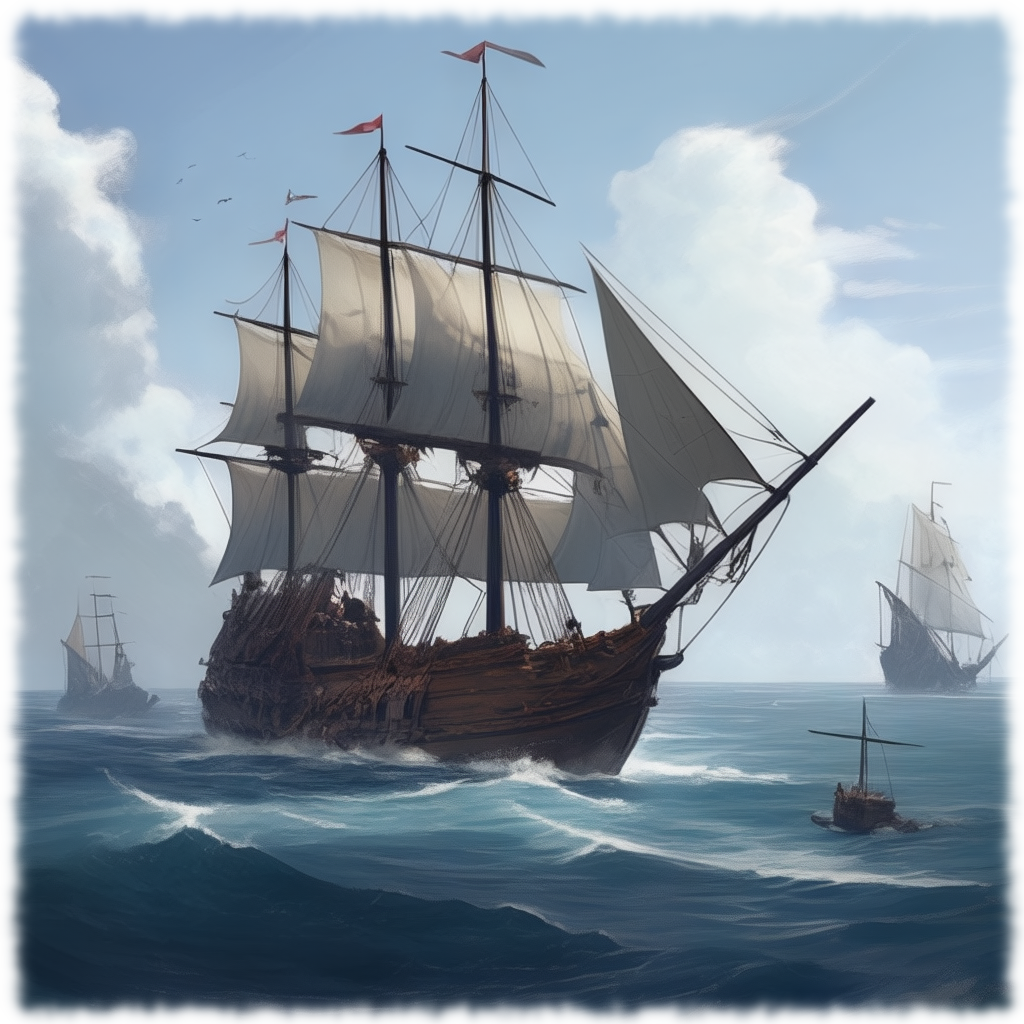
\includegraphics[scale=0.24]{img/ai-images/ships.png}
\end{center}
\end{figure}

\subsection{Travel}
In normal sailing conditions, a sailing vessel can move 20 miles per day per knot of speed. Speeds given are averages. Very  favourable  conditions – for example a  good  strong wind in the desired direction of travel (possibly magically arranged) – can double these speeds. As can a rowing crew who critical their Rowing skill test. 

On the other hand, if a ship is becalmed, with no wind at all, it cannot move.

Every day out of sight of land there is a 5\% chance of a storm. Storms do 2D6 structure points of damage to a ship; a ship reduced to zero structure points begins to sink (and will sink almost instantly if its structure points are reduced to the negative of the original amount). Further, sailors on deck must make Dodge tests to stay on board; a sailor swept overboard and not immediately rescued must make an Athletics test to survive.

Fortunately, the captain can make a Sailing test (modified by manoeuvrability) to halve damage from a storm. Better yet, it is possible to plot a course to avoid an incoming storm if it is detected in time (perhaps using magic or skills such as Natural Lore).

\subsection{Naval Combat}
We consider two ranges of distance between ships.

\subsubsection{Contact}
The vessels can see each other. If both vessels wish to close to combat range, or leave contact, this action is of course automatic, and takes about an hour.

If the vessels want different things, roll opposed Sailing tests, as above.

\subsubsection{Combat Range}
Combat between ships is similar to normal combat. Initiative is decided for each ship, rather than between individuals, by saying that the vessel with the better speed goes first.  

A single test is made to fire a ship’s weapons; no defence roll is made against these attacks. If desired, a character can be appointed weapons officer; he oversees the firing of a ship’s weapons.  That character should make a Ranged Combat skill test; if the test succeeds, the ship’s weapons test has a +20\% bonus.

Hand-held weapons are too small to have any effect on an opposing ship, but can be used against those on the decks. Fire is the exception to this rule, being used to set flamable objects, such as decks, and sails, on fire.

The following special manoeuvres can be made by a ship in combat range. One manoeuvre is allowed per round. Each manoeuvre needs a Sailing skill test by the captain, as indicated above.

\subsubsection{Broadside}
If the skill test succeeds, two attacks with a ship’s weapons can be made instead of one.


\subsubsection{Evade}
If the Sailing test succeeds, the opponent cannot use the broadside, ram, or boarding manoeuvres. Further, the vessel can escape combat range (out to contact range) if the other vessel allows it or the Sailing test succeeds as an opposed roll.


\subsubsection{Ram}
The other vessel is rammed if an opposed Sailing test succeeds. A ramming attack does D6 points of damage per mast. If the ship performing this manoeuvre lacks a battering ram, it also takes half the damage inflicted.


\subsubsection{Boarding}
Boarding is possible if an opposed Sailing test succeeds. In this case, the vessels are roped together, and boarding can commence. A free boarding test is allowed immediately after a successful ramming manoeuvre if desired.

If both vessels want to board the other, this is automatic.


%\section{Major Mental Damage}
%This optional rule is best used for Dark Fantasy games, where the tropes of Fantasy are blended with those of Horror. A setting where the characters are Vampire Hunters confronting the dark masters of the night and their minions is a good example of such a game. 

%When characters witness horrific events, the Gamemaster will ask the players to make a Persistence test. Should that fail, then the character has suffered a mental blow so severe their persona has become altered by it. Roll on the Mental Damage Table below to see what kind of effect that the character suffers from. 

%Independent of whether the Persistence test was successful, they must immediately make a Resilience test with a -40\% modifier, or go into shock for 1D4 rounds. 

%\begin{table*}
%\begin{center}
%\caption{Mental Damage Table}
%\label{tab:mental-damage}
%\begin{rpg-table}[|l|X|]
%	\hline
%	\textbf{Roll 1D6}  & \textbf{Effect}\\
%        \hline
%	1 & The shakes – the incident has left you with an uncontrollable but slight and permanent jittery shake. Lose 2 DEX.\\
%	2 & Dislocation – you find it hard to connect with people, it seems easier to remain unfeeling, to simply let things wash right over you. CHA is reduced by 2.\\
%	3 & Losing your rag – suddenly everything and everyone around you is a constant sign of irritation. This irritation you find is best expressed through physical violence. Each time such a situation arises, you must make a Persistence test. Pass and you’ve controlled your rage, fail and you have no recourse but to lash out – either with your fists or any weapons you are carrying.\\
%	4 & Bottling it – when finding yourself in dangerous and stressful situations you have an overwhelming urge to flee, to find safety. Each time such a situation arises, you must make a Persistence test. Pass and you’ve controlled your urge to run, fail and you’ve bottled it totally. \\
%	5 & Nightmares – every night they invade your dreams, forcing you to relive over and over again the things you have witnessed. Sleep becomes almost impossible, a curse rather than a blessing.  CON is reduced by 2.\\
%	6 & Focus – You find yourself having difficulty focusing on the task in hand. Just keeping aware is a struggle. Both POW and INT are reduced by 2.\\
%	\hline
%\end{rpg-table}
%\end{center}
%\end{table*}

%\begin{rpg-examplebox}
%Rurik is helping search a darkened defiled chapel after the party have defeated a group of Ghouls who had taken up residence there. He picks up some sacks that had been left in a corner of the room.  The humidity and heat have done their work on the contents of these bags, turning the contents inside largely to mush. As Rurik lifts the bags, he can feel something solid moving about in that fluid, and realises with a shock that it contains the half-rotten remains for his cousin's head. The Gamemaster rules that this is such a horrific realisation that Rurik must make a Persistence Roll.  

%Rurik has 34\% Persistence. He rolls 51 – a fail. Rurik has been mentally scared by this revelation. He now rolls 1D6 on the Mental Damage Table. He rolls a 5 – from now on his sleep will be plagued by the memory of this instant.  

%Rurik then rolls against his Resilience of 32\%.  He rolls 23 so doesn’t go into shock.  
%\end{rpg-examplebox}

%\subsection{Modifying the Persistence Roll}
%Some monsters are by their very nature more horrific and disturbing than the standard Ghoul or Zombie, such as Greater Demons, Vampire Lords and indescribable monsters of Cosmic Horror. When encountering such leviathans of terror, whose very existence saps the blood from the character’s skin, the Gamemaster may apply a -20\% or even in very rare world threatening circumstances a -40\% modifier to the Persistence Roll.


%\subsection{Spending Hero Points}
%Just as in a Major Wound, characters can spend a Hero Point to avoid the mental damage they would otherwise have incurred. Instead, the character goes into Shock for 1D4 rounds.


%\subsection{Fumbling and Criticals}
%Should your character fumble the Persistence test, then not only do they receive a mental blow but they also go into shock for 1D8 rounds with no chance of a Resilience roll test to avoid.

%Should a character get a critical Persistence, then they have simply shrugged off what has happened and carry on as normal, so a Resilience roll is not required. 


%\subsection{Going into Shock}
%The character becomes numb and unresponsive, can take no further action in combat situations, and can in certain circumstances become a sitting duck. 


\section{Mass Combat}
The following rules can be used if you want a one roll solution to a battle.

Mass combat involves the commanders’ skills of the two opposing sides, modified by the armies involved. The command skills involved are Lore (Military Tactics), and either Influence or Performance.

The actual battle is resolved by opposed Lore (Military Tactics) tests made by the leaders. A successful test means a force inflicts casualties equal to half its size on the opposition. Half of these casualties are deaths; the other half are injuries. These numbers are doubled on a critical success.

Further, the commander of a losing side in a battle must make an Influence or Performance test to prevent a rout. Routing troops either flee in panic, or surrender when they cannot flee. A further 10\% of an army’s numbers are lost in a rout. A critical success on the Influence or Performance test is needed for a force to continue fighting rather than retreating in a more orderly manner. If a force has nowhere to retreat to, it can continue to fight.

The Lore (Military Tactics) test is modified by various situational factors:
\begin{rpg-list}
\item Better equipped than enemy: +20\% bonus.
\item Better trained than enemy: +20\% bonus.
\item Has significant special forces (e.g. artillery, cavalry, combat mages) that the enemy lacks: +20\% bonus for each.
\item Outnumber enemy by two to one or more: +20\% bonus.
\item Outnumber enemy by four to one or more: +40\% bonus.
\item Enemy in defensive position: -20\% penalty.
\item Enemy fortifications: -40\% penalty.
\item Player character heroics (eg: taking out significant enemy, capturing strategic position): +20\% bonus, or -20\% penalty if attempted heroics go horribly wrong.
\end{rpg-list}

Larger forces might split into several armies, each with their own commander. The rules are still as above, but each army must pick another force to attack.


%\section{Hero Points for Plot Edits}
%In Fantasy Crux it is usually the Gamemaster who describes the situation the player characters find themselves in and the outcome of any skill test. This optional rule allows the player to take control of the narrative and change the direction that the story is going in by spending Hero Points. 
%\begin{description}
%\item[1 point for a minor edit:] changes small details in favour of the player. For example, the player character suddenly has an important item of equipment that they previously forgot to bring with them on the adventure, or the guard forgets to lock the door to the dungeon that the characters are imprisoned in.
%\item[2 points for a major edit:] puts the player character at an advantage. For example, not only is the dungeon door open but the jail guard is asleep at his table.
%\item[3 points for a drastic edit:] something dramatic and almost impossible happens to put the player character at a major advantage. For example, the king trips up on his flowing robes and, as he falls over, he brings down the three bodyguards who are standing close by, giving the player character assassin a clear bow shot at the tyrant.
%\item[5 points for an implausible edit:] the player stretches the boundaries of plausibility (even within a fantasy setting), to advantage. For example, a passing dragon swoops down and attacks the castle the player characters are imprisoned in, allowing them to escape as the guards are busy fighting off the flying fire-breathing reptile.
%\end{description}
%Plot edits must always come with sensible narration from the player so that even with the five point implausible edit must not break the group’s suspension of disbelief. The Gamemaster has the final say on whether a plot edit is allowed or not.

%Players should not rely on plot edits to constantly overcome obstacles, but save them for moments where they are truly stuck or have a cool situation in mind.

%Plot edits may never completely remove obstacles such as opposing characters or imposing physical challenges, but they can be used to temporarily give players the upper hand. For example you can’t use a plot edit to remove a mountain range or instantly kill a major recurring villain, but you can use one to have your player character find an obscure mountain pass or have the villain temporarily knocked unconscious.

\begin{figure}
\begin{center}
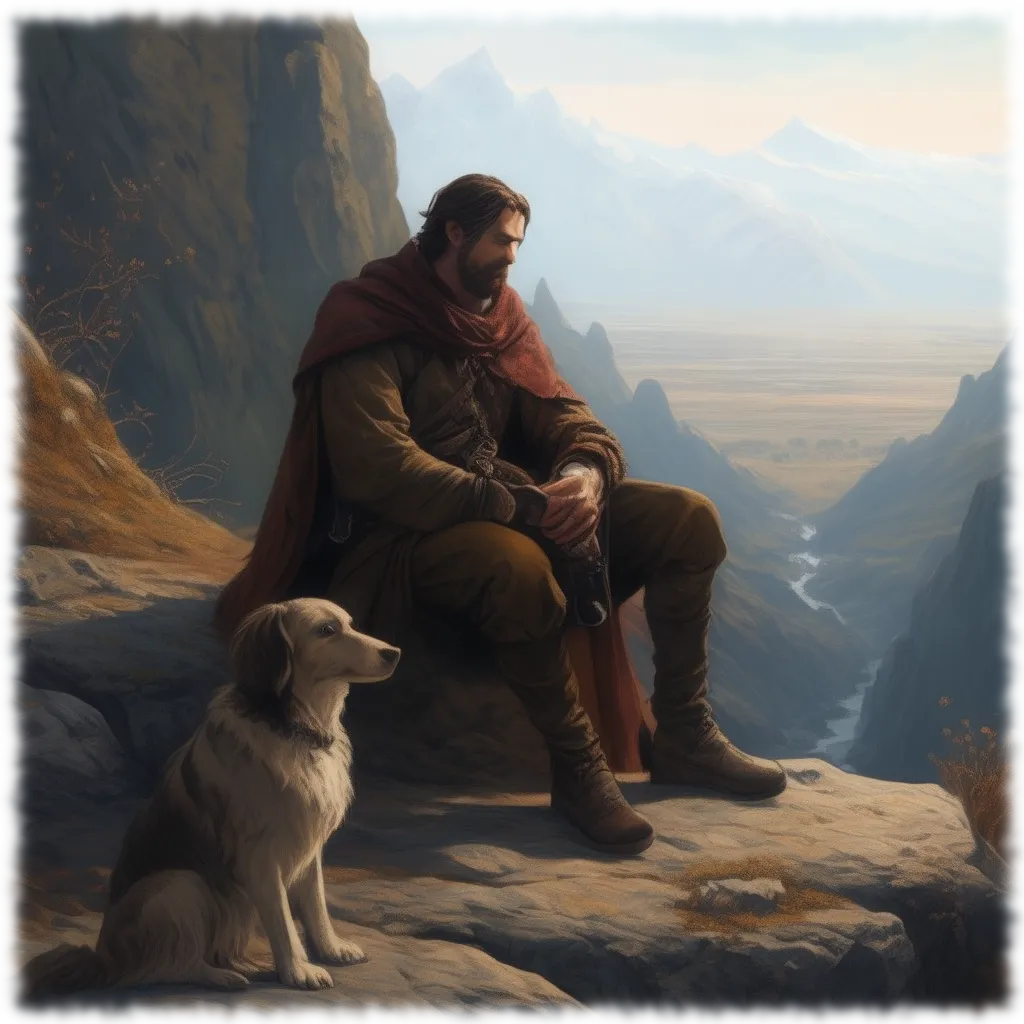
\includegraphics[scale=0.24]{img/ai-images/man-with-dog.png}
\end{center}
\end{figure}


\section{Skill Tests}

\subsection{When to Test}
When the outcome of the character’s action is in doubt or they want to push themselves beyond their expected capacity. If it’s not clear that a character can perform a task, then Gamemaster is well within their rights to call for a skill test.

When it is dramatically appropriate and raises tension in the game. Think carefully before asking for a skill test. Skill tests should be like those moments in a thriller where you are on the edge of your seat and the story could go either way. If the overall result of asking for a skill test is that it will provide the player a success of minor import, such as a minor scrap of information on a Lore roll, just give the player the success without asking them to roll. If the situation is more life or death, describe it as such, highlighting the tension, and ask for a skill test. Where there are definite consequences to a failed skill test, such as falling down a pit filled with spikes if an Athletics skill test is failed, the player should be warned before the character risks taking the action.

\subsection{When not to Test}
As a replacement for good story telling and roleplaying. If the game is flowing nicely as a result of the players and Gamemaster engaging in conversation and weaving a strong exciting story which is keeping everyone happy and entertained through roleplaying, then think twice about breaking that mood by asking for a skill test.

Simply to provide drama and tension in game. The Gamemaster should never substitute a good description of the scene that the players find themselves in, for a series of dice rolls.  

If a similar skill test has just been made. It is tempting to ask for a series of skill tests to simulate a difficult or arduous task, such as climbing an especially difficult cliff, or tracking an opponent through a dense jungle. Don’t. All this does is break player immersion in the game, creating frustration and boredom as several meaningless rolls are made. Instead, ask for a single skill test and modify it to reflect the difficulty of the task. Do not ask for another until the circumstances significantly change.

%\subsection{Creating New Skills}
%Although the Fantasy Crux skill list has been designed to be as concise and complete as possible, during play or during the design of non-player characters for adventures, there may arise a desire to create new skills to describe a previously undiscovered ability. Before introducing a new skill, either by Gamemaster design or player request, consider these two points.

%Is this skill really meaningful and distinct in its own right? Or is it something that can be included in an existing skill?


\section{Fantasy Races}
Most fantasy campaigns will have exotic races as Player Character options. The exact nature of these races will depend on the campaign itself, e.g. Elves in the Tolkien saga are quite different than Elves in the Greyhawk campaign setting.

The Creatures chapter introduction (page~\pageref{ch:creatures}) explains how any creature could be used as a base to create Player Characters. However, a lot of them would not be balanced and the Gamemaster needs to be careful on what races will be allowed in the campaign.

However, some races like Elves, Dwarves or Lizardmen are quite straightforward. Note that when those races have special abilities (e.g. Elves have Night Sight and are Exceptional Archers) they have to spend some of their initial Improvement Points to get that race. That would keep it more balanced for Human characters. Gamemasters have the final say as usual. The following sections contain Elves and Dwarves as examples. 

\subsection{Elves}
The creature entry for Elves (page~\pageref{creature:elf}) has their average Characteristics as well as the dice rolled for the Random Characteristics method. For the point method the starting Characteristics will be analogous to their dice. For example: STR 6, CON 8, DEX 10, SIZ 6, INT 10, POW 8 and CHA 8. Players would then allocate 30 points on top of that.

Remember that the racial top is the maximum possible value plus 3. Thus, Elves can reach a maximum of DEX 27 but only STR 18.

Finally, Elves have Night Sight and are Exceptional Archers. These are useful abilities that would cost 3 Improvement Points each and thus Elf characters will have no extra Improvement Points available during creation.

\subsection{Dwarves}
The creature entry for Dwarves (page~\pageref{creature:dwarf}) has their average Characteristics as well as the dice rolled for the Random Characteristics method. For the point method the starting Characteristics will be analogous to their dice. For example: STR 8, CON 14, DEX 6, SIZ 4, INT 8, POW 8 and CHA 8. Players would then allocate 30 points on top of that.

Remember that the racial top is the maximum possible value plus 3. Thus, Dwarves can reach a maximum of STR and CON of 27.

Finally, Dwarves have Thermoception and Earth Sense. Thermoception is pretty powerful so the player would need to spend 4 Improvement Points to get it. Earch Sense is situational and 2 Improvement Points would be enough. Thus Dwarf characters will have no extra Improvement Points available during creation.



\section{Player Archetypes}

The rules allow for an incredible variety of player character concepts. Everything a player can think can be accommodated with the provided rules. To this end, common magic (see chapter~\ref{ch:magic}) can be used to emulate new abilities as supernatural feats rather than consider them as Magic (since some players will not want to use Magic as it conflicts with their character's concept). In this section we provide one such example by describing how a Monk character could be designed.

\subsection{Concept: Monk}
Characters trained in the monastic traditions will be able to achieve some supernatural feats. These characters will go through extensive training to learn special techiques to represent what they have learned in the monastery.

\begin{figure}[H]
\begin{center}
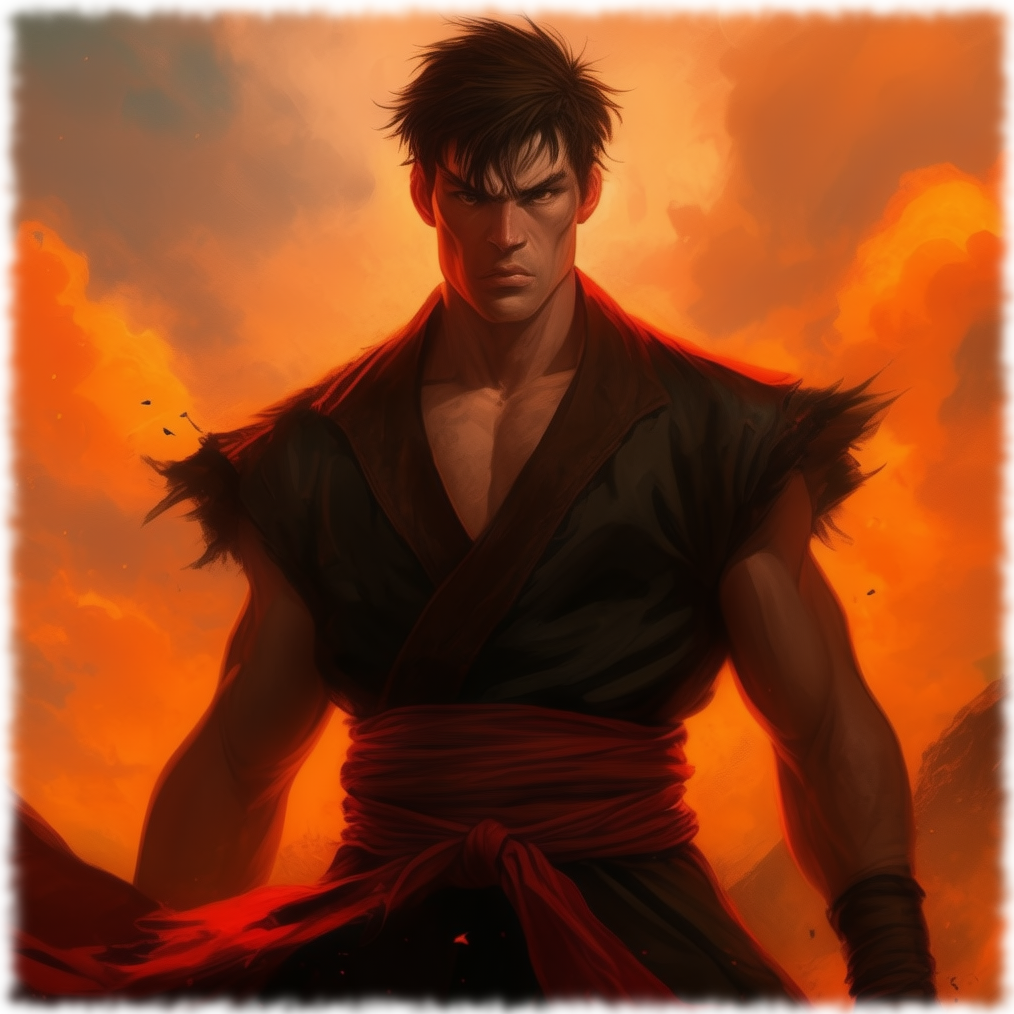
\includegraphics[scale=0.24]{img/ai-images/monk.png}
\end{center}
\end{figure}

\subsubsection{Rules}
The Player can, of course, use the Battle discipline to improve his fighting abilities but to emulate some of the special monk abilities we can use the Magic discipline. The Player needs to pay Improvement Points to get the Magic discipline and then pay IPs for each Magnitude of spells he is learning. The rules and maximum Magnitude they can learn is exactly as the Magic discipline. The Player character will not be casting spells but all the effects of spell casting need to be emulated. For example it should be obvious for anyone that is seeing the Monk that he is initiating something and under duress they may not succeed.

Flavour is important, so the abilities can be named accordingly. For example, the Player could pay to get the `Monastic' discipline and then learn individual monastic `feats'. Achieving a specific feat requires intense focus and meditation and sometimes distractions might cause failure (explaining why the `Monastic' or `Ki Focus' skill check is required).

\subsubsection{Feats}
The following example feats (spells) can be learned from the monastery: Coordination, Cover Blind Side, Cushion Fall, Extra Defense, Fist of the Wind, Flying Kick, Heal, Ironmind, Leap, Mobility, Multi Attack, Resist (Element), Spirit Shield, Strength, and Weapon Enhance.

Note, however, that they can only be applied to `self' and never to others.


%\subsection{Concept: Druid}

%\subsection{Concept: Elementalist}


\section{Traits, Talents, Feats}

Certain campaign concepts might allow characters to get some extraordinary or supernatural abilities without focusing on a specific discipline. Maybe the character wants some special talent interwoven with his background and the Gamemaster allows him, only once during character creation, to get such an ability. Maybe even later under certain circumstances. Or, more simply, it might be possible to add magical runes or tattoos to characters that allow them to manifest certain powers.

\subsection{Rules}
To enable such mechanics Gamemasters might allow certain Magic spells to be cast as a spell-like ability once per day, or more. This is similar to how permanent charms are created with the Create Charms spell.

The player spends three Improvement Points per Magnitude to enable them to use the spell as an ability once per day (1/day); without requiring a Magic Casting skill or any Power. It can be activated as an Action. 

The player spends ten Improvement Points per Magnitude to have the effect of the spell always active. This is quite powerful and care must be taken. In any case, not all spells can be used for such talents and the Gamemaster has the final say.


\section{Minor NPCs}
This does not necessarily mean weak non-player characters. They are just NPCs not important enough to have a proper description. It can be used as an aid when improvising NPCs during play but they are primarily useful to quickly describe minor NPCs in writing.

The description comprises a brief description of the NPC followed by their specialty skill, followed by the items and/or abilities. Typically minor NPCs have 10 HPs and 10 Combat Order but the Gamemaster can increase, when appropriate.

Skills closely related to the description are at the specialty skill level and all other skills at -10\% increments depending on how relevant they are. Effectively, the Gamemaster needs to reduce the skill level as appropriate for the role envisioned.

\vspace{1em}
\begin{rpg-examplebox}	
Human Guard 50 (Shortsword 1D6+1, Leather 2)
\end{rpg-examplebox}

This guard is quite good at his job. He could have 50\% in Close Combat and 50\% in Perception. He could have 40\% in Dodge, Resilience and Ranged Weapons but only 30\% in Persistence. Other skills would be even lower.
The guard is armed with a Shortsword and wears Leather armour which gives 2 AP.

Another example of an elven scholar demonstrates the potential skills more.

\vspace{1em}
\begin{rpg-examplebox}
Elven Scholar 70 (Dagger 1D4+1, 2gp, Amulet of Protection 2)
\end{rpg-examplebox}

The scholar could have 70\% in a couple of Lore skills and/or Languages but only 40\% in her Close Combat skill. She could have a 60\% Persistence or even Healing, etc.
Also note how her magical amulet containing a Protection 2 Magic spell is described.

Finally, extraordinary and supernatural abilities can be described with a brief Discipline abbreviation and then the appropriate Powers. For Disciplines, B is for Battle, M is for Magic, AM for Arcane Magic, DM for Divine Magic, etc.

\vspace{1em}
\begin{rpg-examplebox}
Goblin Witch Doctor 60 (Dagger 1D4+1; M: Heal, Scare, Sap Energy)
\end{rpg-examplebox}

The goblin witch doctor could have a 60\% at his Healing Skill and a 50\% in his Magic Casting skill. He probably has a 40\% in Persistence, Resilience and Dodge and knows 3 Magic spells: Heal, Scare and Sap Energy.


\section{Epic Characters}
For a more heroic style of play, where the adventures of the PCs are of a more epic nature (with characters facing off against a whole host of foes, and perhaps becoming the great heroes of their time), the players and the GM might like to implement the following changes, or some variation of, to character creation:

\begin{rpg-list}
	\item Epic Hit Points: The total HPs will equal Size plus Constitution.
	\item Epic Characteristics: The players can allocate 35 points to Characteristics and the maximum is increased to +5 instead of +3.
	\item Epic Skills: The maximum Skill increase at character creation is 50 points instead of 30. Skills at Master level (above 100\%) are increased by 2\% instead of 1\%.
	\item At the end of character generation each character gains an additional 6 Improvement Points to spend as they wish.
\end{rpg-list}

\begin{figure}
\begin{center}
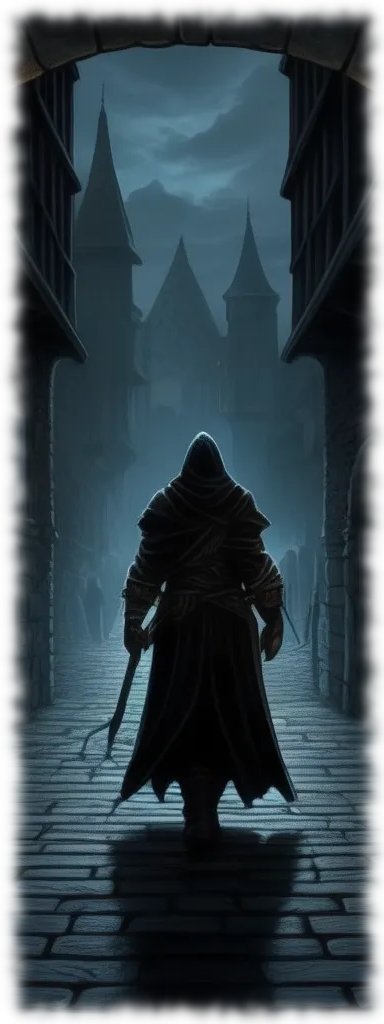
\includegraphics[scale=0.65]{img/ai-images/thief.png}
\end{center}
\end{figure}

\chapter{Creatures}
\label{ch:creatures}

In Fantasy D100, monsters can be as richly detailed as the characters themselves. As well as characteristics they have skills, weapons and supernatural abilities. They are not mere cannon fodder to be killed and looted. They have their own motives that often bring them into conflict with the player characters, and if sentient can be used to create player characters.

This chapter is split into two lists. The first is the Monster List, which is full of creatures fantastic and magical. The second is the Animals List, a smaller list which details more mundane creatures, which the characters may encounter or commonly use as mounts and beasts of burden. Note that just only a sample of the most characteristic monsters are described here. Game masters should consult other D100 supplements (e.g. from Open Quest) to get more ready-made monsters. It is encouraged that Game Masters create campaign-specific monsters using this section's material as examples.
\vspace{1em}

\begin{rpg-titlebox}{Monsters as Player Characters}
Although in theory many of the monsters in this chapter can be used as player characters the following are especially suited: Dwarf, Elf, Centaur, Goblin, Orc, Ogre, Lizard Man.
\end{rpg-titlebox}
  
The following characteristics, attributes, skills, and special rules, collectively known as a ‘Stat block’, for each of the creatures listed on the Monsters List, are the bare bones of a creature. You can use them straight away to give an average non-descript member of that race.

To create creatures that truly fit the adage “Monsters are People too”, take the Stat block and use it as a base for a complete character. Think of a concept for the character and then add the skills, characteristics and supernatural abilities that the character needs. You may want to generate the creature character as if it was a player character. This often creates good opposition for the players, since the creature will be of comparable experience. 

Note that you should be careful with increasing encounter difficulty by increasing numbers of monsters. A much better way is to increase the power of individual monsters, by increasing skills and supernatural abilities, to be closer to the player character power level.  Fantasy D100 combat works best when there is roughly the same amount of monsters as player characters.

\clearpage

\section{Animals}

This list describes more mundane animals. It lists domestic animals (such as horses and dogs), as well as wild beasts. Some of the animals are in their ‘Giant’ form, which are more threatening opponents than their normal species.

None of the animals listed here have any treasure by design. They may have some as determined by the Games Master as fits the needs of the story. For example a carnivore may have a few trinkets In the remains of its previous meals.

All the Animals listed here are of fixed INT and therefore not sentient. They have a Dodge, Persistence and Resilience of DEX x3, Pow x3, CON x3 respectively and none of them know have any supernatural abilities.

\vspace{1em}

\begin{samepage}
\begin{monsterbox}{Ant (Giant)}
	\basics[%
        hitpoints  = 12, 
	majorwound = 6,
	damagemodifier = 0,
	powerpoints = 6,
	movementrate = 15m,
	armor = Chitin (5 AP),
	]
	\rpghline%
	\stats[ % This stat command will autocomplete the modifier for you
		STR = 4D6   (14),
		CON = 3D6+6 (17),
		DEX = 2D6+6 (13),
		SIZ = 2D6   (7),
		INT = 2     (2),
		POW = 1D6+3 (6),
		CHA = 5     (5)
	]
	%\rpghline%
	%\details[%
	% If you want to use commas in these sections, enclose the
	% description in braces.
	% I'm so sorry.
	%languages = {Common Lisp, Erlang},
	%]
	\rpghline%
	\rpgmonstersection{Skills}
	\begin{rpg-monsteraction}[Unarmed Combat 50\%]
		Bite (1D6)
	\end{rpg-monsteraction}
\end{monsterbox}
\end{samepage}


\begin{samepage}
\begin{monsterbox}{Bear}
	\basics[%
        hitpoints  = 19, 
	majorwound = 10,
	damagemodifier = 0,
	powerpoints = 11,
	movementrate = 23m,
	armor = Tough hide (3 AP),
	]
	\rpghline%
	\stats[ % This stat command will autocomplete the modifier for you
		STR = 3D6+15 (25),
		CON = 2D6+6  (13),
		DEX = 3D6    (11),
		SIZ = 3D6+15 (25),
		INT = 5     (5),
		POW = 3D6   (11),
		CHA = 5     (5)
	]
	%\rpghline%
	%\details[%
	% If you want to use commas in these sections, enclose the
	% description in braces.
	% I'm so sorry.
	%languages = {Common Lisp, Erlang},
	%]
	\rpghline%
	\rpgmonstersection{Skills}
	\begin{rpg-monsteraction}[Unarmed Combat 60\%]
		Bite (1D8+2D6), Claw (1D6+2D6)
	\end{rpg-monsteraction}
\end{monsterbox}
\end{samepage}

\begin{samepage}
\begin{monsterbox}{Bull}
	\basics[%
        hitpoints  = 15, 
	majorwound = 8,
	damagemodifier = +1D6,
	powerpoints = 7,
	movementrate = 15m,
	armor = Hide (2 AP),
	]
	\rpghline%
	\stats[ % This stat command will autocomplete the modifier for you
		STR = 4D6+6 (20),
		CON = 2D6+9 (15),
		DEX = 2D6   (7),
		SIZ = 2D6+9 (15),
		INT = 4     (4),
		POW = 2D6   (7),
		CHA = 4     (4)
	]
	%\rpghline%
	%\details[%
	% If you want to use commas in these sections, enclose the
	% description in braces.
	% I'm so sorry.
	%languages = {Common Lisp, Erlang},
	%]
	\rpghline%
	\rpgmonstersection{Skills}
	\begin{rpg-monsteraction}[Unarmed Combat 40\%]
		Charge (1D8+1D6), Trample (1D8+1D6)
	\end{rpg-monsteraction}
\end{monsterbox}
\end{samepage}


\begin{samepage}
\begin{monsterbox}{Crocodile}
	\basics[%
        hitpoints  = 15, 
	majorwound = 8,
	damagemodifier = +1D6,
	powerpoints = 11,
	movementrate = {7m, 2m in water},
	armor = Thich hide (5 AP),
	]
	\rpghline%
	\stats[ % This stat command will autocomplete the modifier for you
		STR = 5D6+12 (30),
		CON = 3D6+12 (19),
		DEX = 3D6    (11),
		SIZ = 4D6    (14),
		INT = 3      (3),
		POW = 3D6    (11),
		CHA = 3      (3)
	]
	%\rpghline%
	%\details[%
	% If you want to use commas in these sections, enclose the
	% description in braces.
	% I'm so sorry.
	%languages = {Common Lisp, Erlang},
	%]
	\rpghline%
	\rpgmonstersection{Skills}
	\begin{rpg-monsteraction}[Unarmed Combat 50\%]
		Bite (1D8+1D6)
	\end{rpg-monsteraction}
\end{monsterbox}
\end{samepage}


\begin{samepage}
\begin{monsterbox}{Dog}
	\basics[%
        hitpoints  = 7, 
	majorwound = 4,
	damagemodifier = 0,
	powerpoints = 9,
	movementrate = 23m,
	armor = None,
	]
	\rpghline%
	\stats[ % This stat command will autocomplete the modifier for you
		STR = 2D6+6 (13),
		CON = 3D6   (11),
		DEX = 2D6+6 (13),
		SIZ = 1D6   (3),
		INT = 5     (5),
		POW = 1D6+6 (9),
		CHA = 5     (5)
	]
	%\rpghline%
	%\details[%
	% If you want to use commas in these sections, enclose the
	% description in braces.
	% I'm so sorry.
	%languages = {Common Lisp, Erlang},
	%]
	\rpghline%
	\rpgmonstersection{Skills}
	\begin{rpg-monsteraction}[Unarmed Combat 40\%]
		Bite (1D6)
	\end{rpg-monsteraction}
\end{monsterbox}
\end{samepage}


\begin{samepage}
\begin{monsterbox}{Elephant}
	\basics[%
        hitpoints  = 36, 
	majorwound = 18,
	damagemodifier = +5D6,
	powerpoints = 13,
	movementrate = 23m,
	armor = Thick hide (3 AP),
	]
	\rpghline%
	\stats[ % This stat command will autocomplete the modifier for you
		STR = 6D6+24 (45),
		CON = 3D6+15 (24),
		DEX = 3D6    (11),
		SIZ = 6D6+30 (48),
		INT = 6      (6),
		POW = 2D6+6  (13),
		CHA = 5      (5)
	]
	%\rpghline%
	%\details[%
	% If you want to use commas in these sections, enclose the
	% description in braces.
	% I'm so sorry.
	%languages = {Common Lisp, Erlang},
	%]
	\rpghline%
	\rpgmonstersection{Skills}
	\begin{rpg-monsteraction}[Unarmed Combat 45\%]
		Trample (1D12+5D6), Tusk (1D10+5D6)
	\end{rpg-monsteraction}
\end{monsterbox}
\end{samepage}

\begin{samepage}
\begin{monsterbox}{Hawk}
	\basics[%
        hitpoints  = 3, 
	majorwound = 2,
	damagemodifier = -1D6,
	powerpoints = 7,
	movementrate = {15m, 30m flying},
	armor = None,
	]
	\rpghline%
	\stats[ % This stat command will autocomplete the modifier for you
		STR = 1D3    (2),
		CON = 2D3    (4),
		DEX = 3D6+18 (27),
		SIZ = 1D2    (2),
		INT = 4      (4),
		POW = 2D6    (7),
		CHA = 4      (4)
	]
	%\rpghline%
	%\details[%
	% If you want to use commas in these sections, enclose the
	% description in braces.
	% I'm so sorry.
	%languages = {Common Lisp, Erlang},
	%]
	\rpghline%
	\rpgmonstersection{Skills}
	\begin{rpg-monsteraction}[Unarmed Combat 50\%]
		Claw (1D6-1D6), Bite (1D4-1D6)
	\end{rpg-monsteraction}
\end{monsterbox}
\end{samepage}


\begin{samepage}
	\begin{monsterbox}{Hawk (Giant)}
	\basics[%
        hitpoints  = 36, 
	majorwound = 18,
	damagemodifier = +4D6,
	powerpoints = 11,
	movementrate = {23m, 30m flying},
	armor = Thick feathers (3 AP),
	]
	\rpghline%
	\stats[ % This stat command will autocomplete the modifier for you
		STR = 6D6+21 (39),
		CON = 5D6+15 (33),
		DEX = 3D6+9  (18),
		SIZ = 6D6+21 (39),
		INT = 4      (4),
		POW = 3D6    (11),
		CHA = 4      (4)
	]
	%\rpghline%
	%\details[%
	% If you want to use commas in these sections, enclose the
	% description in braces.
	% I'm so sorry.
	%languages = {Common Lisp, Erlang},
	%]
	\rpghline%
	\rpgmonstersection{Skills}
	\begin{rpg-monsteraction}[Unarmed Combat 80\%]
		Claw (1D8+4D6), Bite (1D6+4D6)
	\end{rpg-monsteraction}
\end{monsterbox}
\end{samepage}


\begin{samepage}
\begin{monsterbox}{Horse}
	\basics[%
        hitpoints  = 21, 
	majorwound = 11,
	damagemodifier = +2D6,
	powerpoints = 11,
	movementrate = 30m,
	armor = Hide (2 AP),
	]
	\rpghline%
	\stats[ % This stat command will autocomplete the modifier for you
		STR = 2D6+18 (25),
		CON = 3D6+6  (17),
		DEX = 2D6+3  (10),
		SIZ = 2D6+18 (25),
		INT = 4      (4),
		POW = 3D6    (11),
		CHA = 5      (5)
	]
	%\rpghline%
	%\details[%
	% If you want to use commas in these sections, enclose the
	% description in braces.
	% I'm so sorry.
	%languages = {Common Lisp, Erlang},
	%]
	\rpghline%
	\rpgmonstersection{Skills}
	\begin{rpg-monsteraction}[Unarmed Combat 40\%]
		Kick (1D6+2D6)
	\end{rpg-monsteraction}
\end{monsterbox}
\end{samepage}


\begin{samepage}
\begin{monsterbox}{Lion (Big Cat)}
	\basics[%
        hitpoints  = 15, 
	majorwound = 8,
	damagemodifier = +1D6,
	powerpoints = 11,
	movementrate = 23m,
	armor = Hide (2 AP),
	]
	\rpghline%
	\stats[ % This stat command will autocomplete the modifier for you
		STR = 3D6+12 (24),
		CON = 3D6    (11),
		DEX = 3D6+6  (17),
		SIZ = 2D6+12 (19),
		INT = 5      (5),
		POW = 3D6    (11),
		CHA = 5      (5)
	]
	%\rpghline%
	%\details[%
	% If you want to use commas in these sections, enclose the
	% description in braces.
	% I'm so sorry.
	%languages = {Common Lisp, Erlang},
	%]
	\rpghline%
	\rpgmonstersection{Skills}
	\begin{rpg-monsteraction}[Unarmed Combat 60\%]
		Bite (1D8+1D6), Claw (1D6+1D6)
	\end{rpg-monsteraction}
\end{monsterbox}
\end{samepage}


\begin{samepage}
\begin{monsterbox}{Lizard (Giant)}
	\basics[%
        hitpoints  = 15, 
	majorwound = 8,
	damagemodifier = +1D6,
	powerpoints = 11,
	movementrate = 15m,
	armor = Hide (2 AP),
	]
	\rpghline%
	\stats[ % This stat command will autocomplete the modifier for you
		STR = 2D6+12 (19),
		CON = 3D6    (11),
		DEX = 1D6+12 (15),
		SIZ = 2D6+12 (19),
		INT = 3      (3),
		POW = 3D6    (11),
		CHA = 3      (3)
	]
	%\rpghline%
	%\details[%
	% If you want to use commas in these sections, enclose the
	% description in braces.
	% I'm so sorry.
	%languages = {Common Lisp, Erlang},
	%]
	\rpghline%
	\rpgmonstersection{Skills}
	\begin{rpg-monsteraction}[Unarmed Combat 35\%]
		Bite (1D6+1D6), Tail (1D8+1D6)
	\end{rpg-monsteraction}
\end{monsterbox}
\end{samepage}


\begin{samepage}
\begin{monsterbox}{Octupus (Giant)}
	\basics[%
        hitpoints  = 31, 
	majorwound = 16,
	damagemodifier = +4D6,
	powerpoints = 11,
	movementrate = {7m land, 30m swimming},
	armor = Tough skin (4 AP),
	]
	\rpghline%
	\stats[ % This stat command will autocomplete the modifier for you
		STR = 12D6  (42),
		CON = 4D6+6 (14),
		DEX = 3D6+12 (23),
		SIZ = 12D6   (42),
		INT = 4      (4),
		POW = 3D6    (11),
		CHA = 4      (4)
	]
	%\rpghline%
	%\details[%
	% If you want to use commas in these sections, enclose the
	% description in braces.
	% I'm so sorry.
	%languages = {Common Lisp, Erlang},
	%]
	\rpghline%
	\rpgmonstersection{Skills}
	\begin{rpg-monsteraction}[Unarmed Combat 50\%]
		Bite (1D8+4D6), Arm (1D4+4D6)
	\end{rpg-monsteraction}
\end{monsterbox}
\end{samepage}


\begin{samepage}
\begin{monsterbox}{Python (Giant)}
	\basics[%
        hitpoints  = 11, 
	majorwound = 6,
	damagemodifier = +2D6,
	powerpoints = 11,
	movementrate = 15m,
	armor = Scales (3 AP),
	]
	\rpghline%
	\stats[ % This stat command will autocomplete the modifier for you
		STR = 3D6+24 (35),
		CON = 3D6    (11),
		DEX = 2D6+6  (13),
		SIZ = 3D6    (11),
		INT = 3      (3),
		POW = 3D6    (11),
		CHA = 3      (3)
	]
	%\rpghline%
	%\details[%
	% If you want to use commas in these sections, enclose the
	% description in braces.
	% I'm so sorry.
	%languages = {Common Lisp, Erlang},
	%]
	\rpghline%
	\rpgmonstersection{Skills}
	\begin{rpg-monsteraction}[Unarmed Combat 50\%]
		Bite (1D4+2D6), Constrict (1D8+2D6)
	\end{rpg-monsteraction}
\end{monsterbox}
\end{samepage}


\begin{samepage}
\begin{monsterbox}{Rhinoceros}
	\basics[%
        hitpoints  = 19, 
	majorwound = 10,
	damagemodifier = +2D6,
	powerpoints = 11,
	movementrate = 23m,
	armor = Thick hide (5 AP),
	]
	\rpghline%
	\stats[ % This stat command will autocomplete the modifier for you
		STR = 2D6+21 (26),
		CON = 3D6    (11),
		DEX = 2D6    (7),
		SIZ = 2D6+21 (26),
		INT = 3      (3),
		POW = 3D6    (11),
		CHA = 3      (3)
	]
	%\rpghline%
	%\details[%
	% If you want to use commas in these sections, enclose the
	% description in braces.
	% I'm so sorry.
	%languages = {Common Lisp, Erlang},
	%]
	\rpghline%
	\rpgmonstersection{Skills}
	\begin{rpg-monsteraction}[Unarmed Combat 50\%]
		Bite (1D6+2D6), Gore (1D8+2D6), Trample (1D12+2D6)
	\end{rpg-monsteraction}
\end{monsterbox}
\end{samepage}


\begin{samepage}
\begin{monsterbox}{Spider (Giant)}
	\basics[%
        hitpoints  = 22, 
	majorwound = 11,
	damagemodifier = +1D6,
	powerpoints = 11,
	movementrate = {15m on land, 23m in web},
	armor = Chitin (4 AP),
	]
	\rpghline%
	\stats[ % This stat command will autocomplete the modifier for you
		STR = 2D6+12 (19),
		CON = 3D6+6  (17),
		DEX = 2D6+9  (16),
		SIZ = 4D6+12 (26),
		INT = 8      (8),
		POW = 3D6    (11),
		CHA = 2      (2)
	]
	%\rpghline%
	%\details[%
	% If you want to use commas in these sections, enclose the
	% description in braces.
	% I'm so sorry.
	%languages = {Common Lisp, Erlang},
	%]
	\rpghline%
	\rpgmonstersection{Skills}
	\begin{rpg-monsteraction}[Unarmed Combat 50\%]
		Bite (1D6+1D6+Venom), Web
	\end{rpg-monsteraction}
	\rpgmonstersection{Abilities}
	\begin{rpg-monsteraction}[Spider Venom]\\
		\textit{Type:} Ingested or smeared\\
		\textit{Delay:} 1D3 Combat Rounds\\
		\textit{Potency:} Spider's CONx3\\
		\textit{Full Effect:} 1D3 Hit Points per minute and applies –6 penalty to victim’s DEX (upon reaching 0 DEX victim becomes paralysed)\\ 
		\textit{Duration:} 6D10 minutes
	\end{rpg-monsteraction}
	\begin{rpg-monsteraction}[Web]
		Entangles opponent. Success is determined by an opposed check of attack roll vs an Athletics roll. If entangled, the web can be destroyed (POWx2 Hit Points).
	\end{rpg-monsteraction}


\end{monsterbox}
\end{samepage}


\begin{samepage}
\begin{monsterbox}{Viper}
	\basics[%
        hitpoints  = 7, 
	majorwound = 4,
	damagemodifier = 0,
	powerpoints = 13,
	movementrate = 30m,
	armor = Scales (1 AP),
	]
	\rpghline%
	\stats[ % This stat command will autocomplete the modifier for you
		STR = 2D6+6  (13),
		CON = 2D6    (6),
		DEX = 3D6+18 (27),
		SIZ = 2D6    (7),
		INT = 3      (3),
		POW = 2D6+6  (13),
		CHA = 3      (3)
	]
	%\rpghline%
	%\details[%
	% If you want to use commas in these sections, enclose the
	% description in braces.
	% I'm so sorry.
	%languages = {Common Lisp, Erlang},
	%]
	\rpghline%
	\rpgmonstersection{Skills}
	\begin{rpg-monsteraction}[Unarmed Combat 60\%]
		Bite (1D6+Venom)
	\end{rpg-monsteraction}
	\rpgmonstersection{Abilities}
	\begin{rpg-monsteraction}[Viper Venom]\\
		\textit{Type:} Ingested or smeared\\
		\textit{Delay:} 1 Combat Round\\
		\textit{Potency:} 48\\
		\textit{Full Effect:} 1D4 Hit Points damage for each minute and -3 CON (upon reaching 0 CON victim dies)\\ 
		\textit{Duration:} 6D10 minutes
	\end{rpg-monsteraction}
\end{monsterbox}
\end{samepage}


\begin{samepage}
\begin{monsterbox}{Wolf}
	\basics[%
        hitpoints  = 12, 
	majorwound = 6,
	damagemodifier = 0,
	powerpoints = 11,
	movementrate = 23m,
	armor = None,
	]
	\rpghline%
	\stats[ % This stat command will autocomplete the modifier for you
		STR = 3D6   (11),
		CON = 3D6+3 (14),
		DEX = 3D6+3 (13),
		SIZ = 2D6+3 (10),
		INT = 5     (5),
		POW = 3D6   (11),
		CHA = 5     (5)
	]
	%\rpghline%
	%\details[%
	% If you want to use commas in these sections, enclose the
	% description in braces.
	% I'm so sorry.
	%languages = {Common Lisp, Erlang},
	%]
	\rpghline%
	\rpgmonstersection{Skills}
	\begin{rpg-monsteraction}[Unarmed Combat 50\%]
		Bite (1D8), Claw (1D6)
	\end{rpg-monsteraction}
\end{monsterbox}
\end{samepage}

\clearpage

\section{Monsters}


\begin{monsterbox}{Basilisk}
	\textit{Born from the egg of a cockerel acted upon in an Alchemist’s or witches cauldron, this magical monster is the product of foul magic. It is a large lizard with multicoloured scales. Its baleful gaze can kill and its blood is poisonous and corrosive.   Basilisks are usually employed as guardians of their master’s treasure.}\\
	\rpghline
	\basics[%
        hitpoints  = 8, %\rpgdice{3d8 + 3},
	majorwound = 4,
	damagemodifier = -1D6,
	powerpoints = 16,
	movementrate = 15m,
	armor = Armor Scales (2AP),
	plunderrating = 5
	]
	\rpghline%
	\stats[ % This stat command will autocomplete the modifier for you
		STR = 2D3   (4),
		CON = 2D6+6 (13),
		DEX = 3D6   (11),
		SIZ = 1D3   (2),
		INT = 3     (3),
		POW = 1D6+12 (16),
		CHA = 3     (3)
	]
	%\rpghline%
	%\details[%
	% If you want to use commas in these sections, enclose the
	% description in braces.
	% I'm so sorry.
	%languages = {Common Lisp, Erlang},
	%]
	\rpghline%
	\rpgmonstersection{Skills}
	\begin{rpg-monsteraction}[Resistances]
		Dodge~40\%, Persistence~50\%, Resilience~70\%
	\end{rpg-monsteraction}
	\begin{rpg-monsteraction}[Knowledge]
    		Natural lore~40\%
	\end{rpg-monsteraction}
	\begin{rpg-monsteraction}[Practical]
		Athletics~65\%, Deception~40\%
	\end{rpg-monsteraction}
	\begin{rpg-monsteraction}[Ranged Combat 100\%]
		Death Gaze (Range: POW in metres)
	\end{rpg-monsteraction}
	\begin{rpg-monsteraction}[Unarmed Combat 35\%]
		Bite (1D6-1D6+poison)
	\end{rpg-monsteraction}
	\rpgmonstersection{Abilities}
	\begin{rpg-monsteraction}[Basilisk Venom \& Poison Blood]\\
		\textit{Type:} Ingested or smeared\\
		\textit{Delay:} Immediate\\
		\textit{Potency:} 65\\
		\textit{Full Effect:} 1D4 Hit Points damage for each minute and -6 CON (upon reaching 0 CON victim dies)\\ 
		\textit{Duration:} 6D10 minutes\\
		Any non-magical weapon hitting the basilisk corrodes in the creature’s blood, completely disintegrating after D4 rounds. The basilisk’s poison and corrosive blood are magical effects, which lose their special properties a few minutes after leaving the basilisk’s body, making it virtually impossible to use the creature as a source for making lethal compounds.
	\end{rpg-monsteraction}
	\begin{rpg-monsteraction}[Death Gaze]
		A basilisk can kill with a glance. In combat the basilisk glares at a single opponent each round. If the basilisk overcomes the target in an opposed test of its Persistence against the target’s Resilience, the target dies instantly. Using the gaze attack costs no Power Points, and the basilisk may attack normally in any round in which it uses the gaze attack. This attack penetrates magical defences as if it were a Magnitude 6 Magic spell. If the target successfully resists the gaze attack, he is unharmed, though he may certainly be targeted again. 
	\end{rpg-monsteraction}

\end{monsterbox}

\newpage


\begin{monsterbox}{Centaur}
	\textit{Atop of the body of a well-bred and strong horse, this creature has the body of a strong athletic human where the horse’s head should be. The centaur is the raw power and nobility of nature incarnate. Often they act as the self styled protectors of the wilderness, which brings them into conflict with more settled races who encroach on their territory.}\\
	\rpghline
	\basics[%
        hitpoints  = 19, %\rpgdice{3d8 + 3},
	majorwound = 10,
	damagemodifier = +1D6,
	powerpoints = 11,
	movementrate = 23m,
	armor = Leather (2AP),
	plunderrating = 2
	]
	\rpghline%
	\stats[ % This stat command will autocomplete the modifier for you
		STR = 3D6+6 (17),
		CON = 3D6   (11),
		DEX = 3D6+3 (14),
		SIZ = 4D6+12 (26),
		INT = 2D6+6 (13),
		POW = 3D6   (11),
		CHA = 3D6   (11)
	]
	%\rpghline%
	%\details[%
	% If you want to use commas in these sections, enclose the
	% description in braces.
	% I'm so sorry.
	%languages = {Common Lisp, Erlang},
	%]
	\rpghline%
	\rpgmonstersection{Skills}
	\begin{rpg-monsteraction}[Resistances]
		Dodge~30\%, Persistence~45\%, Resilience~60\%
	\end{rpg-monsteraction}
	\begin{rpg-monsteraction}[Knowledge]
    		Natural lore~60\%
	\end{rpg-monsteraction}
	\begin{rpg-monsteraction}[Practical]
		Athletics~60\%, Performance~50\%, Perception~40\%, Deception~30\%
	\end{rpg-monsteraction}
	\begin{rpg-monsteraction}[Ranged Combat 70\%]
		Longbow (1D10+1D6)
	\end{rpg-monsteraction}
	\begin{rpg-monsteraction}[Close Combat 40\%]
		Lance (1D10+1D6), Medium Shield (1D6+1D6), Arming Sword (1D8+1D6)
	\end{rpg-monsteraction}
	\begin{rpg-monsteraction}[Unarmed Combat 40\%]
		Kick (1D6+1D6)
	\end{rpg-monsteraction}
	\rpgmonstersection{Abilities}
	\begin{rpg-monsteraction}[Supernatural]
		Typically supernatural abilities that are related to Battle, Earth and Nature are available to Centaurs.
	\end{rpg-monsteraction}
	\begin{rpg-monsteraction}[Exceptional Archers]
		Centaurs can use their damage modifier when using bows.
	\end{rpg-monsteraction}

\end{monsterbox}

\newpage


\begin{monsterbox}{Dragon}
	\textit{These giant flying reptilian monsters are incredibly powerful and dangerous. Dragons are very individual in their temperament. Some are evil cruel beasts. Others are solitary hoarding creatures. Some use their high intelligence to lord it over lesser races.}\\
	\rpghline
	\basics[%
        hitpoints  = 50, %\rpgdice{3d8 + 3},
	majorwound = 25,
	damagemodifier = +7D6,
	powerpoints = 26,
	movementrate = {30m, 45m when flying},
	armor = Dragon Scales (12AP),
	plunderrating = 5-6
	]
	\rpghline%
	\stats[ % This stat command will autocomplete the modifier for you
		STR = 20D6    (70),
		CON = 10D6    (35),
		DEX = 4D6     (14),
		SIZ = 10D6+30 (65),
		INT = 6D6     (21),
		POW = 4D6+12  (26),
		CHA = 6D6     (21)
	]
	%\rpghline%
	%\details[%
	% If you want to use commas in these sections, enclose the
	% description in braces.
	% I'm so sorry.
	%languages = {Common Lisp, Erlang},
	%]
	\rpghline%
	\rpgmonstersection{Skills}
	\begin{rpg-monsteraction}[Resistances]
		Dodge~30\%, Persistence~180\%, Resilience~120\%
	\end{rpg-monsteraction}
	\begin{rpg-monsteraction}[Knowledge]
		Natural lore~100\%, Culture (local) 100\%
	\end{rpg-monsteraction}
	\begin{rpg-monsteraction}[Practical]
		Athletics~120\%, Influence~150\%, Perception~110\%
	\end{rpg-monsteraction}
	\begin{rpg-monsteraction}[Unarmed Combat 125\%]
		Bite (1D10+7D6), Claw (1D8+7D6), Tail (1D20+7D6)
	\end{rpg-monsteraction}
	\rpgmonstersection{Abilities}
	\begin{rpg-monsteraction}[Double Claw Attack]
		In a single Combat Round a dragon can make two claw attacks.
	\end{rpg-monsteraction}
	\begin{rpg-monsteraction}[Breathe Flame]
		The Dragon may breathe flame over an area as a Combat Action. The flame will cover a cone in front of the Dragon, which stretches for its POW in metres. At its furthest extent, the cone is equal to the creature’s POW in width.
		Any creature caught in the flame suffers 4D6 fire damage, though on a successful Dodge roll a character may dive for cover to halve this damage and AP counts as normal.
		The Dragon may only breathe flame once per hour. Further attempts to breathe flame within this time period require the creature to make a Resilience test, with a cumulative –20\% penalty for every attempt.
	\end{rpg-monsteraction}
	\begin{rpg-monsteraction}[Supernatural]
		Dragons are highly magical creatures and often learn Arcane Magic and Magic (of which they have a minimum of 10 points of Magnitude of spells)
	\end{rpg-monsteraction}
\end{monsterbox}

\newpage



\begin{monsterbox}{Dwarf}
	\textit{These short, stocky and bearded, human-like creatures, live underground in vast halls, meticulously carved out of the rock by their highly skilled hands.  Long lived and proud of their work, Dwarfs are the natural enemies of Orcs and Goblins, who often encroach upon their realms.}\\
	\rpghline
	\basics[%
        hitpoints  = 15, %\rpgdice{3d8 + 3},
	majorwound = 8,
	damagemodifier = 0,
	powerpoints = 11,
	movementrate = 12m,
	armor = Chainmail (5AP),
	plunderrating = 3
	]
	\rpghline%
	\stats[ % This stat command will autocomplete the modifier for you
		STR = 4D6   (14),
		CON = 2D6+12 (19),
		DEX = 3D6   (11),
		SIZ = 1D6   (7),
		INT = 2D6+6 (13),
		POW = 3D6   (11),
		CHA = 3D6   (11)
	]
	%\rpghline%
	%\details[%
	% If you want to use commas in these sections, enclose the
	% description in braces.
	% I'm so sorry.
	%languages = {Common Lisp, Erlang},
	%]
	\rpghline%
	\rpgmonstersection{Skills}
	\begin{rpg-monsteraction}[Resistances]
		Dodge~20\%, Persistence~40\%, Resilience~55\%
	\end{rpg-monsteraction}
	\begin{rpg-monsteraction}[Knowledge]
    		Craft~70\%
	\end{rpg-monsteraction}
	\begin{rpg-monsteraction}[Practical]
		Athletics~50\%, Engineering~35\%, Trade~60\%, Mechanisms~40\%
	\end{rpg-monsteraction}
	\begin{rpg-monsteraction}[Close Combat 65\%]
		War Hammer (1D8), Battleaxe (1D8), Medium Shield (1D6)
	\end{rpg-monsteraction}
	\begin{rpg-monsteraction}[Ranged Combat 45\%]
		Light Crossbow (1D8)
	\end{rpg-monsteraction}
	\rpgmonstersection{Abilities}
	\begin{rpg-monsteraction}[Supernatural]
		Typically supernatural abilities that are related to Battle, Earth and Metals are available to Dwarves.
	\end{rpg-monsteraction}
	\begin{rpg-monsteraction}[Thermoception]
		Dwarves can see at dark as if it was day, by detecting heat and cold.
	\end{rpg-monsteraction}
	\begin{rpg-monsteraction}[Earth Sense]
		Dwarfs can automatically sense how far they are underground and whether or not the tunnels or chambers they are in are structurally sound.
	\end{rpg-monsteraction}

\end{monsterbox}

\newpage

\begin{monsterbox}{Elemental}
	\textit{These are magical beings of raw elemental power that come from the Other Worlds. They are usually called or summoned to the mundane world to do the bidding of Priests and Arcane Magic users. Their appearance can vary. Some representative elementals can be seen below.}\\
	\rpghline
	\rpgmonstersection{Types}
	\begin{rpg-monsteraction}[Undines]
		Water elementals that look like a featureless humanoid made of water whose legs dissolve into a pillar then pool of water.\\
		\textit{Type of attack:} Drown\\
		\textit{Resistance used:} Resilience\\
		\textit{Attribute damage:} Hit Points
	\end{rpg-monsteraction}
	\begin{rpg-monsteraction}[Shades]
    		Darkness elementals that are living blobs of darkness.\\
		\textit{Type of attack:} Fear\\
		\textit{Resistance used:} Persistence\\
		\textit{Attribute damage:} Power Points\\
		Shades attack using Fear, when they reduce their opponent’s Power Point’s total to zero they literally die of shock.
	\end{rpg-monsteraction}
	\begin{rpg-monsteraction}[Salamanders]
		Fire elementals that look like lizards made of fire.\\
		\textit{Type of attack:} Burning\\
		\textit{Resistance used:} Resilience\\
		\textit{Attribute damage:} Hit Points
	\end{rpg-monsteraction}
	\begin{rpg-monsteraction}[Gnomes]
		Earth elementals that look like humanoids made of rock.\\
		\textit{Type of attack:} Crush\\
		\textit{Resistance used:} Resilience\\
		\textit{Attribute damage:} Hit Points
	\end{rpg-monsteraction}
	\begin{rpg-monsteraction}[Sylphs]
		Air elementals that take the form of clouds which fly.\\
		\textit{Type of attack:} Buffet\\
		\textit{Resistance used:} Resilience\\
		\textit{Attribute damage:} Hit Points
	\end{rpg-monsteraction}
	\rpgmonstersection{Abilities}
	\begin{rpg-monsteraction}[Attributes]
		The only Stat that an elemental has is SIZ, all its derived attributes and skills are based on this (see table~\ref{tab:elemental-attributes-skills}). Elementals attack by engulfing their enemies. All opponents within the area of attack are potential targets. Elementals use their Attack percentage, which is equal to their size times five, to hit the target who then resists using the resistance appropriate to the attack.
	\end{rpg-monsteraction}
	\begin{rpg-monsteraction}[Immunities]
		Diseases and Poisons
	\end{rpg-monsteraction}
	\begin{rpg-monsteraction}[See Invisible]
		Elementals have magical senses that allow them to ‘see’ invisible creatures, such as immaterial spirits. They also gain a +40\% when detecting hidden characters.
	\end{rpg-monsteraction}
	\begin{rpg-monsteraction}[Camouflage]
		All elementals have the equivalent of a 80\% Deception when lying next to a environment of the same element as themselves. For example, undines are nearly invisible when lying in a pool of water and Gnomes can curl up and blend into a surrounding rocky area.
	\end{rpg-monsteraction}

\end{monsterbox}

\begin{table*}
\begin{center}
\caption{Elemental Attributes and Skills}
\label{tab:elemental-attributes-skills}
\begin{rpg-table}[|l|c|c|Y|Y|Y|Y|c|c|c|]
	\hline
	\textbf{Size}  & \textbf{SIZ} & \textbf{Damage} & \textbf{Hit Points (=SIZ)} & \textbf{Attack (=SIZx5)} & \textbf{Area of attack (=SIZ/5)} & \textbf{Movement rate} & \textbf{Dodge} & \textbf{Persistence} & \textbf{Resilience}\\
	\hline
	Small     & 3  & 1D6 & 3  & 15\%  & 1m  & 15m & 120 & 30  & 100\\
	Medium    & 9  & 2D6 & 9  & 45\%  & 3m  & 23m & 90  & 60  & 100\\
	Large     & 21 & 3D6 & 21 & 105\% & 7m  & 30m & 60  & 90  & 100\\
	Small     & 50 & 4D6 & 50 & 250\% & 16m & 45m & 30  & 120 & 100\\
	\hline
\end{rpg-table}
\end{center}
\end{table*}


\newpage


\begin{monsterbox}{Elf}
	\textit{Forest dwellers, these creatures are slender and tall, with ears that end in a point. Haughty and proud, they do not suffer the ravages of time like other mortal races. Tightly bound to their forest realms in ways no human can understand, they often come into conflict with those who despoil their lands.}\\
	\rpghline
	\basics[%
        hitpoints  = 11, 
	majorwound = 6,
	damagemodifier = 0,
	powerpoints = 13,
	movementrate = 15m,
	armor = Leather (2AP),
	plunderrating = 1
	]
	\rpghline%
	\stats[ % This stat command will autocomplete the modifier for you
		STR = 2D6+3 (10),
		CON = 3D6   (11),
		DEX = 3D6+6 (17),
		SIZ = 2D6+3 (10),
		INT = 3D6+6 (17),
		POW = 2D6+6 (13),
		CHA = 3D6   (11)
	]
	%\rpghline%
	%\details[%
	% If you want to use commas in these sections, enclose the
	% description in braces.
	% I'm so sorry.
	%languages = {Common Lisp, Erlang},
	%]
	\rpghline%
	\rpgmonstersection{Skills}
	\begin{rpg-monsteraction}[Resistances]
		Dodge~55\%, Persistence~55\%, Resilience~20\%
	\end{rpg-monsteraction}
	\begin{rpg-monsteraction}[Knowledge]
    		Nature lore~80\%
	\end{rpg-monsteraction}
	\begin{rpg-monsteraction}[Practical]
		Athletics~55\%, Deception~55\%, Perception~30\%, Healing~50\%
	\end{rpg-monsteraction}
	\begin{rpg-monsteraction}[Close Combat 60\%]
		Longspear (1D8)
	\end{rpg-monsteraction}
	\begin{rpg-monsteraction}[Ranged Combat 80\%]
		Shortbow (1D8)
	\end{rpg-monsteraction}
	\rpgmonstersection{Abilities}
	\begin{rpg-monsteraction}[Supernatural]
		Typically supernatural abilities that are related to Battle, Healing and Nature are available to Elves.
	\end{rpg-monsteraction}
	\begin{rpg-monsteraction}[Night Sight]
		Elves treat partial darkness as illuminated and darkness as only partial darkness.
	\end{rpg-monsteraction}
	\begin{rpg-monsteraction}[Exceptional Archers]
		Elves can use their damage modifier when using bows.
	\end{rpg-monsteraction}

\end{monsterbox}

\newpage


\begin{monsterbox}{Goblin}
	\textit{Sneakier crueller cousins of the Orcs, goblins are a quarrelsome bunch of green-skinned humanoids. They stand as tall as a human child and their smiling faces are dominated by large hooked noses and mouth full of razor-sharp teeth. Constantly in the shadow of the larger humanoid races, often used as slaves or cannon fodder, these diminutive psychopaths take out their frustration on any other creatures unlucky enough to be outnumbered by them or in their power.}\\
	\rpghline
	\basics[%
        hitpoints  = 9, %\rpgdice{3d8 + 3},
	majorwound = 5,
	damagemodifier = 0,
	powerpoints = 10,
	movementrate = 15m,
	armor = Leather (2AP),
	plunderrating = 1
	]
	\rpghline%
	\stats[ % This stat command will autocomplete the modifier for you
		STR = 2D6+3 (10),
		CON = 2D6+3 (10),
		DEX = 5D6   (17),
		SIZ = 2D6   (7),
		INT = 3D6   (11),
		POW = 2D6+3 (10),
		CHA = 2D6   (7)
	]
	%\rpghline%
	%\details[%
	% If you want to use commas in these sections, enclose the
	% description in braces.
	% I'm so sorry.
	%languages = {Common Lisp, Erlang},
	%]
	\rpghline%
	\rpgmonstersection{Skills}
	\begin{rpg-monsteraction}[Resistances]
		Dodge~50\%, Persistence~20\%, Resilience~35\%
	\end{rpg-monsteraction}
	\begin{rpg-monsteraction}[Knowledge]
    		Natural lore~50\%
	\end{rpg-monsteraction}
	\begin{rpg-monsteraction}[Practical]
		Athletics~50\%, Perception~35\%, Deception~75\%, Mechanisms~50\%
	\end{rpg-monsteraction}
	\begin{rpg-monsteraction}[Close Combat 40\%]
		Shortspear (1D6), Small Shield (1D4)
	\end{rpg-monsteraction}
	\begin{rpg-monsteraction}[Ranged Combat 50\%]
		Sling (1D6)
	\end{rpg-monsteraction}
	\rpgmonstersection{Abilities}
	\begin{rpg-monsteraction}[Supernatural]
		On their own, Goblins can sometimes learn Battle and Magic disciplines (leaders and shamans).
	\end{rpg-monsteraction}
	\begin{rpg-monsteraction}[Thermoception]
		Goblins can see at night as if it was day, by seeing heat and cold.
	\end{rpg-monsteraction}

\end{monsterbox}

\newpage

\begin{monsterbox}{Lizardman}
	\textit{Lizardmen are bipedal Lizards that walk upright, use tools and magic, and would threaten mankind, if they didn’t prefer very hot climates, such as arid deserts and steamy swamps.  They can be found in anything from small primitive groups to large civilisations which enslave humans to build their awesome monuments.}\\
	\rpghline
	\basics[%
        hitpoints  = 11,
	majorwound = 6,
	damagemodifier = +1D4,
	powerpoints = 11,
	movementrate = 15m,
	armor = Scales (2AP),
	plunderrating = 3
	]
	\rpghline%
	\stats[ % This stat command will autocomplete the modifier for you
		STR = 3D6+6 (17),
		CON = 3D6   (11),
		DEX = 2D6+3 (10),
		SIZ = 3D6   (11),
		INT = 2D6+6 (13),
		POW = 3D6   (11),
		CHA = 2D6   (7)
	]
	%\rpghline%
	%\details[%
	% If you want to use commas in these sections, enclose the
	% description in braces.
	% I'm so sorry.
	%languages = {Common Lisp, Erlang},
	%]
	\rpghline%
	\rpgmonstersection{Skills}
	\begin{rpg-monsteraction}[Resistances]
		Dodge~45\%, Persistence~25\%, Resilience~30\%
	\end{rpg-monsteraction}
	\begin{rpg-monsteraction}[Knowledge]
    		Natural lore~45\%
	\end{rpg-monsteraction}
	\begin{rpg-monsteraction}[Practical]
		Athletics~45\%, Deception~30\%, Perception~35\%
	\end{rpg-monsteraction}
	\begin{rpg-monsteraction}[Close Combat 45\%]
		Battleaxe (1D8+1D4)
	\end{rpg-monsteraction}
	\begin{rpg-monsteraction}[Ranged Combat 35\%]
		Sling (1D6)
	\end{rpg-monsteraction}
	\begin{rpg-monsteraction}[Unarmed Combat 25\%]
		Bite (1D6+1D4)
	\end{rpg-monsteraction}
	\rpgmonstersection{Abilities}
	\begin{rpg-monsteraction}[Supernatural]
		Any discipline is available to Lizardmen.
	\end{rpg-monsteraction}

\end{monsterbox}

\newpage

\begin{monsterbox}{Ogre}
	\textit{On first glance ogres look like tall, handsome humans. But their mouth full of sharp canines soon betrays their true nature. They live as small family groups, or as leaders of orc and goblin war bands, and are fiercesome carnivores, preferring the sweet flesh of intelligent creatures.}\\
	\rpghline
	\basics[%
        hitpoints  = 13, %\rpgdice{3d8 + 3},
	majorwound = 7,
	damagemodifier = +1D6,
	powerpoints = 13,
	movementrate = 15m,
	armor = Leather (2AP),
	plunderrating = 3
	]
	\rpghline%
	\stats[ % This stat command will autocomplete the modifier for you
		STR = 2D6+12 (19),
		CON = 2D6+6  (13),
		DEX = 3D6    (11),
		SIZ = 2D6+6  (13),
		INT = 2D6+6  (13),
		POW = 2D6+6  (13),
		CHA = 3D6+3  (14)
	]
	%\rpghline%
	%\details[%
	% If you want to use commas in these sections, enclose the
	% description in braces.
	% I'm so sorry.
	%languages = {Common Lisp, Erlang},
	%]
	\rpghline%
	\rpgmonstersection{Skills}
	\begin{rpg-monsteraction}[Resistances]
		Dodge~35\%, Persistence~55\%, Resilience~35\%
	\end{rpg-monsteraction}
	\begin{rpg-monsteraction}[Knowledge]
		Culture (local human)~60\%
	\end{rpg-monsteraction}
	\begin{rpg-monsteraction}[Practical]
		Athletics~35\%, Deception~30\%, Perception~35\%
	\end{rpg-monsteraction}
	\begin{rpg-monsteraction}[Close Combat 60\%]
		Arming Sword (1D8+1D6), Medium Shield (1D6+1D6), 
	\end{rpg-monsteraction}
	\begin{rpg-monsteraction}[Ranged Combat 40\%]
		Shortbow (1D8)
	\end{rpg-monsteraction}
	\begin{rpg-monsteraction}[Unarmed Combat 60\%]
		Fist (1D3+1D6), Bite (1D4+1D6)
	\end{rpg-monsteraction}
	\rpgmonstersection{Abilities}
	\begin{rpg-monsteraction}[Supernatural]
		Any is possible although they do tend to gravitate towards manipulation and control of others.
	\end{rpg-monsteraction}

\end{monsterbox}

\newpage

\begin{monsterbox}{Ogre (Mutant)}
	\textit{Many ogres follow dark and hideous faiths, their foul practices and evil ways eventually lead to their bodies becoming monstrous and warped. It is hard to believe that these gigantic creatures are related to their seductive, weaker kin. Both types of ogre relish in the taste of human flesh and hunt man with vigour. Mutant ogres are either solitary or the leaders of great clans of other monsters, amongst them might rules.}\\
	\rpghline
	\basics[%
        hitpoints  = 18, %\rpgdice{3d8 + 3},
	majorwound = 9,
	damagemodifier = +2D6,
	powerpoints = 10,
	movementrate = 15m,
	armor = Tough Skin (2AP),
	plunderrating = 1
	]
	\rpghline%
	\stats[ % This stat command will autocomplete the modifier for you
		STR = 3D6+12 (23),
		CON = 2D6+6  (13),
		DEX = 3D6    (11),
		SIZ = 3D6+12 (23),
		INT = 2D6+3  (10),
		POW = 2D6+3  (10),
		CHA = 1D6    (3)
	]
	%\rpghline%
	%\details[%
	% If you want to use commas in these sections, enclose the
	% description in braces.
	% I'm so sorry.
	%languages = {Common Lisp, Erlang},
	%]
	\rpghline%
	\rpgmonstersection{Skills}
	\begin{rpg-monsteraction}[Resistances]
		Dodge~35\%, Persistence~45\%, Resilience~35\%
	\end{rpg-monsteraction}
	\begin{rpg-monsteraction}[Knowledge]
		Nature lore~35\%
	\end{rpg-monsteraction}
	\begin{rpg-monsteraction}[Practical]
		Athletics~35\%, Deception~50\%, Perception~50\%
	\end{rpg-monsteraction}
	\begin{rpg-monsteraction}[Close Combat 60\%]
		Great Axe (2D8+2D6)
	\end{rpg-monsteraction}
	\begin{rpg-monsteraction}[Ranged Combat 40\%]
		Rock (1D6)
	\end{rpg-monsteraction}
	\begin{rpg-monsteraction}[Unarmed Combat 60\%]
		Fist (1D6+2D6), Bite (1D8+2D6)
	\end{rpg-monsteraction}
	\rpgmonstersection{Abilities}
	\begin{rpg-monsteraction}[Supernatural]
		Any is possible as long as it is related to evil and demonic powers.
	\end{rpg-monsteraction}

\end{monsterbox}

\newpage

\begin{monsterbox}{Orc}
	\textit{Foul green-skinned humanoids with pig-like snouts and a foul temper. Orcs live for violence and have a society where the strong dominate the weak. Orc clans, known as warbands, regularly war on each other and other races that they come across.}\\
	\rpghline
	\basics[%
        hitpoints  = 11, %\rpgdice{3d8 + 3},
	majorwound = 6,
	damagemodifier = 0,
	powerpoints = 10,
	movementrate = 15m,
	armor = Leather (2AP),
	plunderrating = 2
	]
	\rpghline%
	\stats[ % This stat command will autocomplete the modifier for you
		STR = 4D6 (14),
		CON = 3D6 (11),
		DEX = 4D6 (14),
		SIZ = 2D6+3 (10),
		INT = 3D6   (11),
		POW = 2D6+3 (10),
		CHA = 2D6   (7)
	]
	%\rpghline%
	%\details[%
	% If you want to use commas in these sections, enclose the
	% description in braces.
	% I'm so sorry.
	%languages = {Common Lisp, Erlang},
	%]
	\rpghline%
	\rpgmonstersection{Skills}
	\begin{rpg-monsteraction}[Resistances]
		Dodge~35\%, Persistence~35\%, Resilience~35\%
	\end{rpg-monsteraction}
	\begin{rpg-monsteraction}[Knowledge]
    		Craft~40\%
	\end{rpg-monsteraction}
	\begin{rpg-monsteraction}[Practical]
		Athletics~35\%, Deception~45\%, Perception~45\%
	\end{rpg-monsteraction}
	\begin{rpg-monsteraction}[Close Combat 40\%]
		Scimitar (1D8), Medium Shield (1D6)
	\end{rpg-monsteraction}
	\begin{rpg-monsteraction}[Ranged Combat 50\%]
		Shortbow (1D8)
	\end{rpg-monsteraction}
	\rpgmonstersection{Abilities}
	\begin{rpg-monsteraction}[Supernatural]
		Orcs usually worship evil or warlike deities and are members of their cults. Exceptional leaders and shamans might be trained in Battle and Magic disciplines respectively.
	\end{rpg-monsteraction}

\end{monsterbox}

\newpage

\begin{monsterbox}{Pixie}
	\textit{Diminutive humanoids with butterfly wings, these mischievous beings live close to nature in forests and woods. They are quite friendly with elves, and other races quite often mistake them as a subspecies of elf.}\\
	\rpghline
	\basics[%
        hitpoints  = 8, 
	majorwound = 4,
	damagemodifier = -1D6,
	powerpoints = 13,
	movementrate = {15m, 30m when flying},
	armor = None,
	plunderrating = 0
	]
	\rpghline%
	\stats[ % This stat command will autocomplete the modifier for you
		STR = 2D3  (4),
		CON = 3D6  (11),
		DEX = 4D6  (14),
		SIZ = 1D6  (4),
		INT = 3D6   (11),
		POW = 2D6+6 (13),
		CHA = 3D6   (11)
	]
	%\rpghline%
	%\details[%
	% If you want to use commas in these sections, enclose the
	% description in braces.
	% I'm so sorry.
	%languages = {Common Lisp, Erlang},
	%]
	\rpghline%
	\rpgmonstersection{Skills}
	\begin{rpg-monsteraction}[Resistances]
		Dodge~60\%, Persistence~60\%, Resilience~20\%
	\end{rpg-monsteraction}
	\begin{rpg-monsteraction}[Knowledge]
    		Nature lore~80\%
	\end{rpg-monsteraction}
	\begin{rpg-monsteraction}[Practical]
		Athletics~60\%, Deception~60\%, Perception~60\%
	\end{rpg-monsteraction}
	\begin{rpg-monsteraction}[Close Combat 10\%]
		Dagger (1D4+1-1D6)
	\end{rpg-monsteraction}
	\begin{rpg-monsteraction}[Ranged Combat 25\%]
		Sling (1D6)
	\end{rpg-monsteraction}
	\rpgmonstersection{Abilities}
	\begin{rpg-monsteraction}[Supernatural]
		Pixies have several supernatural abilities and almost always magic abilities.
	\end{rpg-monsteraction}


\end{monsterbox}

\newpage

\begin{monsterbox}{Skeleton}
	\textit{The animated bones of a human, these are the products of supernatural forces. Skeletons are the lowest type of undead which are often created to and act as disposable warriors and tomb guards.}\\
	\rpghline
	\basics[%
        hitpoints  = 8, 
	majorwound = 4,
	damagemodifier = 0,
	powerpoints = 0,
	movementrate = 15m,
	armor = Leather (2AP),
	plunderrating = 0
	]
	\rpghline%
	\stats[ % This stat command will autocomplete the modifier for you
		STR = 2D6+6 (13),
		CON = 1D6   (4),
		DEX = 3D6   (11),
		SIZ = 3D6   (11),
		INT = 0     (0),
		POW = 0     (0),
		CHA = 0     (0)
	]
	%\rpghline%
	%\details[%
	% If you want to use commas in these sections, enclose the
	% description in braces.
	% I'm so sorry.
	%languages = {Common Lisp, Erlang},
	%]
	\rpghline%
	\rpgmonstersection{Skills}
	\begin{rpg-monsteraction}[Resistances]
		Dodge~10\%, Persistence~100\%, Resilience~100\%
	\end{rpg-monsteraction}
	\begin{rpg-monsteraction}[Close Combat 35\%]
		Arming Sword (1D8), Medium Shield (1D6)
	\end{rpg-monsteraction}
	\rpgmonstersection{Abilities}
	\begin{rpg-monsteraction}[Immunities]
		Skeletons are immune to all diseases, poisons and mind control supernatural abilities.
	\end{rpg-monsteraction}

\end{monsterbox}

\newpage

\begin{monsterbox}{Troll}
	\textit{Standing over two metres tall, the troll is a fearsome humanoid monster with grey-green slimy skin. Its bulging bloodshot eyes, clawed hands and a stooped posture finishes off the grim countenance of this terrifying creature. Its appearance is not only the reason for its evil reputation. The troll has the ability to literally regrow severed limbs, bashed bones and to mend slashed skin, before the eyes of its attackers. Fortunately such creatures are solitary, unless enslaved by other evil humanoids, and of incredibly low intelligence.}\\
	\rpghline
	\basics[%
        hitpoints  = 23, 
	majorwound = 12,
	damagemodifier = +2D6,
	powerpoints = 11,
	movementrate = 23m,
	armor = Tough hide (3AP),
	plunderrating = 1
	]
	\rpghline%
	\stats[ % This stat command will autocomplete the modifier for you
		STR = 4D6+12 (26),
		CON = 3D6+9  (20),
		DEX = 2D6    (7),
		SIZ = 4D6+12 (26),
		INT = 1D6+3  (6),
		POW = 3D6    (11),
		CHA = 2D6    (7)
	]
	%\rpghline%
	%\details[%
	% If you want to use commas in these sections, enclose the
	% description in braces.
	% I'm so sorry.
	%languages = {Common Lisp, Erlang},
	%]
	\rpghline%
	\rpgmonstersection{Skills}
	\begin{rpg-monsteraction}[Resistances]
		Dodge~25\%, Persistence~25\%, Resilience~60\%
	\end{rpg-monsteraction}
	\begin{rpg-monsteraction}[Knowledge]
    		Nature lore~40\%
	\end{rpg-monsteraction}
	\begin{rpg-monsteraction}[Practical]
		Athletics~20\%, Deception~20\%, Perception~20\%
	\end{rpg-monsteraction}
	\begin{rpg-monsteraction}[Close Combat 40\%]
		Club (1D6+2D6)
	\end{rpg-monsteraction}
	\begin{rpg-monsteraction}[Unarmed Combat 40\%]
		Claw (1D6+2D6)
	\end{rpg-monsteraction}
	\rpgmonstersection{Abilities}
	\begin{rpg-monsteraction}[Regeneration]
		Trolls regenerate damage done to them quite quickly, healing 1D6 Hit Points per Combat Round. This regeneration will not work on damage caused by fire.
	\end{rpg-monsteraction}
	\begin{rpg-monsteraction}[Thermoception]
		Trolls can see at night as if it was day, by seeing heat and cold.
	\end{rpg-monsteraction}

\end{monsterbox}

\newpage

\begin{monsterbox}{Wyvern}
	\textit{These giant slender green reptiles are akin to dragons but with no forelegs and animal intelligence.}\\
	\rpghline
	\basics[%
        hitpoints  = 23, 
	majorwound = 12,
	damagemodifier = +2D6,
	powerpoints = 10,
	movementrate = {23m, 30m when flying},
	armor = Scales (5AP),
	plunderrating = 1
	]
	\rpghline%
	\stats[ % This stat command will autocomplete the modifier for you
		STR = 4D6+12 (26),
		CON = 2D6+12 (19),
		DEX = 2D6+6  (13),
		SIZ = 4D6+12 (26),
		INT = 7      (7),
		POW = 3D6    (11),
		CHA = 6      (6)
	]
	%\rpghline%
	%\details[%
	% If you want to use commas in these sections, enclose the
	% description in braces.
	% I'm so sorry.
	%languages = {Common Lisp, Erlang},
	%]
	\rpghline%
	\rpgmonstersection{Skills}
	\begin{rpg-monsteraction}[Resistances]
		Dodge~50\%, Persistence~35\%, Resilience~50\%
	\end{rpg-monsteraction}
	\begin{rpg-monsteraction}[Practical]
		Athletics~50\%, Deception~10\%, Perception~60\%
	\end{rpg-monsteraction}
	\begin{rpg-monsteraction}[Unarmed Combat 60\%]
		Bite (1D10+2D6), Sting (1D6+2D6+poison), Claw (1D6+2D6)
	\end{rpg-monsteraction}
	\rpgmonstersection{Abilities}
	\begin{rpg-monsteraction}[Multiple Attacks]
		In one combat round the Wyvern can use all three attacks.	
	\end{rpg-monsteraction}
	\begin{rpg-monsteraction}[Wyvern Sting Poison]
		\\Type: Ingested\\
		Delay: 1D2 Combat Rounds\\
                Potency: 60\\
		Full Effect: 1D6 damage and -4 penalty to CON\\
		Duration: 6D10 minutes
	\end{rpg-monsteraction}

\end{monsterbox}

\clearpage

\section{Spirits}
\label{sec:spirits}

\begin{samepage}
\begin{monsterbox}{Ancestor Spirit}
	\textit{An Ancestor Spirit is the deceased relation of a living being. They are the keepers of tribal wisdom, ancient advisors or just long lost loved ones. They appear as they did in life, dressed in tattered clothing of familiar designs. Ancestor Spirits often manifest at large gatherings of their kinsmen, at holy rituals or to bring portents of warning and doom to their kin. Some clans bind their ancestors to holy locations, while other see that as disrespectful.}\\
	\rpghline
	\basics[%
	powerpoints = 17,
	movementrate = 30m,
	plunderrating = 0
	]
	\rpghline%
	\stats[ % This stat command will autocomplete the modifier for you
		STR = -,
		CON = -,
		DEX = -,
		SIZ = -,
		INT = 3D6    (11),
		POW = 3D6+6  (17),
		CHA = 3D6    (11)
	]
	%\rpghline%
	%\details[%
	% If you want to use commas in these sections, enclose the
	% description in braces.
	% I'm so sorry.
	%languages = {Common Lisp, Erlang},
	%]
	\rpghline%
	\rpgmonstersection{Skills}
	\begin{rpg-monsteraction}[Resistances]
		Dodge~40\%, Persistence~50\%
	\end{rpg-monsteraction}
	\begin{rpg-monsteraction}[Knowledge]
		Lore (Spirit World)~40\%
	\end{rpg-monsteraction}
	\begin{rpg-monsteraction}[Spirit Combat 40\%]
		Spectral Blast (1D6)
	\end{rpg-monsteraction}
	\rpgmonstersection{Other}
	\begin{rpg-monsteraction}[Special Rules]
		All Ancestor Spirits are capable of covertly possessing their relatives to aid them. All Ancestors know 1D6 X 10\% Skills and have 1D4 points of Magic spells (they may rarely have Arcane or Divine Magic). When they possess their relatives, the Ancestor gives them access to their magic which is cast at POWx4. The skills of the ancestor are added as a bonus to those possessed for the duration of the possession. The skills can be selected at random, but most will have skills logical to the spirits background, the maximum amount of points allocated to one skill is 30\%. Some examples follow.
	\end{rpg-monsteraction}
	\begin{rpg-monsteraction}[Uncle Mad Blood the Pirate Captain]
		\\INT 9 - POW 15 - CHA 10\\
		Skills: Close Combat 20\%, Sailing 20\%\\
                Spells: Weapon Enhance 4
	\end{rpg-monsteraction}

	\begin{rpg-monsteraction}[Granny Goodweather]
		\\INT 17 - POW 20 - CHA 18\\
		Skills: Healing 20\%, Influence 30\%, Natural World 10\%\\
                Spells: Heal 4
	\end{rpg-monsteraction}
\end{monsterbox}
\end{samepage}

%\newpage

\begin{samepage}
\begin{monsterbox}{Disease Spirit}
	\textit{Disease spirits are the source of misery and illness. They appear in a sickly green humanoid form, with a skull or sunken plaid face for a head.
They are commonly encountered in wilderness areas, where there are no Shamans to banish them, and around evil monster groups whose evil Shaman’s bind them to protect their treasure and lair.}\\
	\rpghline
	\basics[%
	powerpoints = 17,
	movementrate = 30m,
	plunderrating = 0
	]
	\rpghline%
	\stats[ % This stat command will autocomplete the modifier for you
		STR = -,
		CON = -,
		DEX = -,
		SIZ = -,
		INT = 2D6    (7),
		POW = 3D6+6  (17),
		CHA = 3D6    (11)
	]
	%\rpghline%
	%\details[%
	% If you want to use commas in these sections, enclose the
	% description in braces.
	% I'm so sorry.
	%languages = {Common Lisp, Erlang},
	%]
	\rpghline%
	\rpgmonstersection{Skills}
	\begin{rpg-monsteraction}[Resistances]
		Dodge~40\%, Persistence~50\%
	\end{rpg-monsteraction}
	\begin{rpg-monsteraction}[Knowledge]
		Lore (Disease)~100\%, Lore (Spirit World)~40\%
	\end{rpg-monsteraction}
	\begin{rpg-monsteraction}[Practical]
		Deception~30\%
	\end{rpg-monsteraction}
	\begin{rpg-monsteraction}[Spirit Combat 50\%]
		Spectral Claw (1D6)
	\end{rpg-monsteraction}
	\begin{rpg-monsteraction}[Special Rules]
		A disease spirit is in essence a disease, either mundane or magical. After covertly possessing its victim, the possessed will be forced to make Resilience tests to resist the effects of the disease (see page \pageref{ssec:disease}). However, the disease cannot be thrown off until the disease spirit is ousted. Also, the spirit will nearly always choose to apply its POW as a penalty to the possessed’s Resilience tests.
		If the possessed dies while being possessed by a disease spirit, there is a percentage chance equal to the spirit’s POW that it will arise as a new disease spirit in 2D6 hours.
	\end{rpg-monsteraction}
\end{monsterbox}
\end{samepage}

%\newpage 

\begin{samepage}
\begin{monsterbox}{Guardian Spirit}
	\textit{These spirits are often found guarding treasures, tombs and temples. They are unusual in that they are bound to a location or object, but remain discorporate. They take many forms, such as leonine monster guard dogs, shadowy robed figures or pale warriors. The Guardian Spirit has conditions set upon it as part of its binding determining how it will defend its post. When these conditions are broken the spirit lets out a screaming howl and then attacks in Spirit Combat. The warning howl can be heard at a distance of 10m per point of the Guardian’s POW. A Guardian cannot roam from its post a distance greater than its POW in meters.}\\
	\rpghline
	\basics[%
	powerpoints = 17,
	movementrate = 30m,
	plunderrating = (depends on the Treasure being guarded)
	]
	\rpghline%
	\stats[ % This stat command will autocomplete the modifier for you
		STR = -,
		CON = -,
		DEX = -,
		SIZ = -,
		INT = 2D6    (7),
		POW = 3D6+6  (17),
		CHA = 3D6    (11)
	]
	%\rpghline%
	%\details[%
	% If you want to use commas in these sections, enclose the
	% description in braces.
	% I'm so sorry.
	%languages = {Common Lisp, Erlang},
	%]
	\rpghline%
	\rpgmonstersection{Skills}
	\begin{rpg-monsteraction}[Resistances]
		Dodge~40\%, Persistence~60\%
	\end{rpg-monsteraction}
	\begin{rpg-monsteraction}[Knowledge]
		Lore (Spirit World)~40\%
	\end{rpg-monsteraction}
	\begin{rpg-monsteraction}[Spirit Combat 70\%]
		Spectral Claw (1D6)
	\end{rpg-monsteraction}
\end{monsterbox}
\end{samepage}

%\newpage 

\begin{samepage}
\begin{monsterbox}{Healing Spirit}
	\textit{The nemesis of the disease spirit this spirit appears as a bright happily glowing orb. They are typically summoned to help heal the sick and wounded.}\\
	\rpghline
	\basics[%
	powerpoints = 14,
	movementrate = 30m,
	plunderrating = 0
	]
	\rpghline%
	\stats[ % This stat command will autocomplete the modifier for you
		STR = -,
		CON = -,
		DEX = -,
		SIZ = -,
		INT = 2D6    (7),
		POW = 4D6    (14),
		CHA = 3D6    (11)
	]
	%\rpghline%
	%\details[%
	% If you want to use commas in these sections, enclose the
	% description in braces.
	% I'm so sorry.
	%languages = {Common Lisp, Erlang},
	%]
	\rpghline%
	\rpgmonstersection{Skills}
	\begin{rpg-monsteraction}[Resistances]
		Dodge~40\%, Persistence~50\%
	\end{rpg-monsteraction}
	\begin{rpg-monsteraction}[Knowledge]
		Lore (Disease)~100\%, Lore (Spirit World)~60\%
	\end{rpg-monsteraction}
	\begin{rpg-monsteraction}[Spirit Combat 50\%]
		Spectral Blast (1D6)
	\end{rpg-monsteraction}
	\begin{rpg-monsteraction}[Magic 100\%]
		Heal 6
	\end{rpg-monsteraction}
	\begin{rpg-monsteraction}[Special Rules]
		The natural enemy of a disease spirit, a healing spirit is only capable of entering Spirit Combat with a disease spirit already covertly possessing a creature. If the healing spirit can bring the disease spirit to zero Power Points, it will force it to leave its host. The healing spirit will then depart as well, for it cannot permanently possess any creature. If a healing spirit is used on an individual who is sick from a mundane illness (rather than from a disease spirit), it will add its POW as a percentage bonus to the individual’s chance of success on his next Resilience test to throw off the effects of the disease.
	\end{rpg-monsteraction}
\end{monsterbox}
\end{samepage}

%\newpage 

\begin{samepage}
\begin{monsterbox}{Magic Spirit}
	\textit{Magic spirits are spirits that have mastery of one or more spells. If bound, the holder of the spirit may use the spirit’s Power Points for casting spells. Magic spirits may not initiate Spirit Combat, but may use the spells it knows to attack or defend itself. They appear as a series of multi-coloured orbs equal in number to the number of spells they know.}\\
	\rpghline
	\basics[%
	powerpoints = 14,
	movementrate = 30m,
	plunderrating = 0
	]
	\rpghline%
	\stats[ % This stat command will autocomplete the modifier for you
		STR = -,
		CON = -,
		DEX = -,
		SIZ = -,
		INT = 3D6    (11),
		POW = 4D6    (14),
		CHA = 1D6    (4)
	]
	%\rpghline%
	%\details[%
	% If you want to use commas in these sections, enclose the
	% description in braces.
	% I'm so sorry.
	%languages = {Common Lisp, Erlang},
	%]
	\rpghline%
	\rpgmonstersection{Skills}
	\begin{rpg-monsteraction}[Resistances]
		Dodge~40\%, Persistence~50\%
	\end{rpg-monsteraction}
	\begin{rpg-monsteraction}[Knowledge]
		Lore (Spirit World)~60\%
	\end{rpg-monsteraction}
	\begin{rpg-monsteraction}[Spirit Combat 50\%]
		Spectral Blast (1D6)
	\end{rpg-monsteraction}
	\begin{rpg-monsteraction}[Magic]
		A magic spirit knows 1D6 Magic, Divine Magic or Arcane Magic spells. These spirits will only know one  spell type – for example, a magic spirit will not have both Divine and Arcane spells, nor may it ever learn spells of another type. If the spirit casts Divine Magic, it must regain the use of spent spells in the same way a Priest does. If casting Arcane Magic or Magic it has a casting skill equal to its POW x 5.
	\end{rpg-monsteraction}
\end{monsterbox}
\end{samepage}

%\newpage 

\begin{samepage}
\begin{monsterbox}{Passion Spirit}
	\textit{This group of spirits embody negative and harmful feelings and emotions. If they successfully defeat a living creature in Spirit Combat, they will covertly possess that creature. The results of this possession depend upon the particular passion spirit. They are normally invisible, but fear spirits appear as an inky black form with a skull head, madness spirits are ghost like with faces quickly changing from one expression to another while pain spirits take on an angry red form with a face twisted in agony.}\\
	\rpghline
	\basics[%
	powerpoints = 17,
	movementrate = 30m,
	plunderrating = 0
	]
	\rpghline%
	\stats[ % This stat command will autocomplete the modifier for you
		STR = -,
		CON = -,
		DEX = -,
		SIZ = -,
		INT = 2D6+3  (10),
		POW = 3D6+6  (17),
		CHA = 4D6    (14)
	]
	%\rpghline%
	%\details[%
	% If you want to use commas in these sections, enclose the
	% description in braces.
	% I'm so sorry.
	%languages = {Common Lisp, Erlang},
	%]
	\rpghline%
	\rpgmonstersection{Skills}
	\begin{rpg-monsteraction}[Resistances]
		Dodge~40\%, Persistence~50\%
	\end{rpg-monsteraction}
	\begin{rpg-monsteraction}[Knowledge]
		Lore (Spirit World)~60\%
	\end{rpg-monsteraction}
	\begin{rpg-monsteraction}[Spirit Combat 55\%]
		Spectral Claw (1D6)
	\end{rpg-monsteraction}
	\rpgmonstersection{Other}
	\begin{rpg-monsteraction}[Fear Spirit]
		If a fear spirit covertly possesses a host, the host becomes permanently Demoralised (as the Magic spell), until the spirit is cast out.
	\end{rpg-monsteraction}
	\begin{rpg-monsteraction}[Madness Spirit]
		If a madness spirit succeeds in covertly possessing a victim, it will manifest itself in daily bouts of insanity. At least once per day, the madness spirit will attempt to cause an insane fit in its host. It matches its Persistence against the host’s Resilience in a standard opposed test. If the host succeeds, the madness spirit will be quiescent for at least a number of hours equal to the host’s POW. If the host fails, he becomes incapacitated for 1D20 hours – screaming madly, giggling incoherently or simply becoming catatonic for the duration of the effect. The madness spirit chooses the manner of madness, though most are partial to a single effect. The madness spirit will also attempt to assert itself whenever its host is in a stressful situation. Combat is an obvious example, but these spirits also delight in affecting their hosts in a variety of other stressful, important situations – collapsing into a fit of mad giggling while petitioning an unfriendly king for a boon is exactly the kind of thing madness spirits enjoy. Note that if the stressful situation occurs during a period of forced quiescence on the part of the spirit, it will be unable to manifest itself.
	\end{rpg-monsteraction}
	\begin{rpg-monsteraction}[Pain Spirit]
		If a pain spirit manages to covertly possess its target, the victim will be overcome with a sudden burst of pain. From that point on, until the spirit is cast out, the victim will always be conscious of a dull ache in his joints or a twinge in his muscles. Whenever the host acts quickly (as in combat) or concentrates (as in spell casting), and sometimes purely at random intervals, he is struck by a sudden spasm of pain. This pain reduces all the host’s skill tests by a penalty equal to the spirit’s POW.
	\end{rpg-monsteraction}
\end{monsterbox}
\end{samepage}

%\newpage




\appendix
% licenses
\newpage

OPEN GAME LICENSE  Version 1.0a

The following text is the property of Wizards of the Coast Inc. and is Copyright 2000 Wizards of the Coast, Inc ('Wizards'). All Rights Reserved.



\onecolumn
\chapter{Acknowledgements and Art}


%\begin{scriptsize}
\noindent I am grateful to Stability AI for their excellent work with Stable Cascade that allowed me to make most of the art.

\vspace{1em}

\noindent I would also like to thank my friend John Malis that he allowed me to use some of his 3D textures as fillers throughout the book.

\vspace{1em}

\noindent All of the art in this book is under the Creative Commons Attribution-Noncommercial-No Derivative Works 3.0 License (CC-NC-ND-v3).

\vspace{1em}

\noindent The CC-NC-ND-v3 license is available at: https://creativecommons.org/licenses/by-nc-nd/3.0/
%\end{scriptsize}


% End document
\end{document}
